% TODO next Iteration
% - ref-prefixes: sec, py, img, eq
% - refnumbers within section
% - \Tsys, \Xsig, \Ysig makros
% - factboxes
% - index terms
\documentclass[ngerman]{article}
%
\usepackage[fleqn]{amsmath}
\usepackage{amsfonts, amssymb, yhmath}
\usepackage{amsthm}
\usepackage{thmtools}
\usepackage{bm}
\usepackage{graphicx}
\usepackage[]{pgfplots}
\pgfplotsset{compat=newest}

%% end packages
%% 

\declaretheorem[
	numberwithin=section,
  title=Lemma,
  refname={lemma,lemmas},
  Refname={Lemma,Lemmas}
]{Lem}

\declaretheorem[
	numberwithin=section,
  title=Theorem,
  refname={theorem,theorems},
  Refname={Theorem,Theorems}
]{Thm}

\declaretheorem[
	numberwithin=section,
  title=Corollary,
  refname={corollary,corollaries},
  Refname={Corollary,Corollaries}
]{Cor}

\declaretheorem[
	numberwithin=section,
  title=Example,
  refname={example,examples},
  Refname={Example,Examples}
]{Exm}

\declaretheorem[
	numberwithin=section,
  title=Remark,
  refname={remark,remarks},
  Refname={Remark,Remarks}
]{Rem}

\declaretheorem[
	numberwithin=section,
  title=Algorithm,
  refname={algorithm,algorithms},
  Refname={Algorithm,Algorithms}
]{Alg}

\declaretheorem[
	numberwithin=section,
  title=Definition,
  refname={definition,definitions},
  Refname={Definition,Definitions}
]{Def}

\declaretheorem[
	numberwithin=section,
  title=Discussion,
  refname={discussion,discussions},
  Refname={Discussion,Discussions}
]{Dis}

\newcommand{\Ind}[1]{{\boldsymbol{\mathrm{#1}}}}

\newcommand{\trans}{\mathrm{T}}
\newcommand{\herm}{\mathrm{H}}
\newcommand{\forward}[2]{\bm{\phi}_{#1}(#2)}
\newcommand{\backward}[2]{\bm{\beta}_{#1}(#2)}

\newcommand{\R}{\mathbb{R}}
\newcommand{\C}{\mathbb{C}}
\newcommand{\K}{\mathbb{K}}
\newcommand{\N}{\mathbb{N}}
\newcommand{\Z}{\mathbb{Z}}
\newcommand{\PP}{\mathbb{P}}
\newcommand{\Ps}[1]{{\mathfrak{P}\left( #1\right)}}
\newcommand{\As}{\mathcal{A}}
\newcommand{\Hs}{\mathcal{H}}
\newcommand{\Fs}{\mathcal{F}}
\newcommand{\Gs}{\mathcal{G}}
\newcommand{\Ts}{\mathcal{T}}
\newcommand{\Li}{\mathcal{L}}
\newcommand{\RT}{{\mathscr{R}}}
\newcommand{\FT}{{\mathscr{F}}}
\newcommand{\BT}{{\mathscr{B}}}
\newcommand{\HT}{{\mathscr{H}}}

\newcommand{\Real}[1]{{\rm Re}\left\{#1\right\}}
\newcommand{\Imag}[1]{{\rm Im}\left\{#1\right\}}
\newcommand{\Conj}[1]{\overline{#1}}

\newcommand{\E}{\bm{\mathrm{E}}}
\newcommand{\Prb}{\bm{\mathrm{P}}}

\newcommand{\ScPr}[2]{{\left\langle #1,#2 \right\rangle}}
\newcommand{\Norm}[1]{{\left\Vert #1\right\Vert}}
\newcommand{\Abs}[1]{{\left| #1 \right|}}
\newcommand{\Text}[1]{{\hspace{3mm} \text{#1} \hspace{3mm}}}
\newcommand{\brac}[2]{{\left(\frac{#1}{#2}\right)}}
\newcommand{\br}[1]{{\left(#1\right)}}

\newcommand{\Int}[4]{{\int\limits_{#1}^{#2}{#3}\,\mathrm{d}{#4}}}
\newcommand{\Sum}[3]{{\sum\limits_{#1}^{#2}{#3}}}
\newcommand{\Prod}[3]{{\prod\limits_{#1}^{#2}{#3}}}
\newcommand{\SumB}[3]{{\left(\sum\limits_{#1}^{#2}{#3}\right)}}
\newcommand{\ProdB}[3]{{\left(\prod\limits_{#1}^{#2}{#3}\right)}}

\newcommand{\ConvA}[2]{{\xrightarrow[]{#1 \rightarrow #2}}}
\newcommand{\RA}[1]{\overset{#1}{\Rightarrow}}
\newcommand{\LRA}[1]{\overset{#1}{\Leftrightarrow}}
\newcommand{\V}[0]{\hspace{1.2mm}\middle\vert\hspace{1.5mm}}
\newcommand{\D}[0]{\hspace{0.5mm}:\hspace{1.0mm}}

\DeclareMathOperator*{\Argmin}{argmin}
\DeclareMathOperator*{\Argmax}{argmax}
\DeclareMathOperator*{\Arg}{arg}
\DeclareMathOperator*{\BlkDiag}{blkdiag}
\DeclareMathOperator*{\Conv}{conv}
\DeclareMathOperator*{\Cov}{Cov}
\DeclareMathOperator*{\Cone}{cone}
\DeclareMathOperator*{\Diag}{diag}
\DeclareMathOperator*{\id}{id}
\DeclareMathOperator*{\Ker}{ker}
\DeclareMathOperator*{\Median}{median}
\DeclareMathOperator*{\Max}{max}
\DeclareMathOperator*{\Mat}{mat}
\DeclareMathOperator*{\Min}{min}
\DeclareMathOperator*{\Mod}{Mod}
\DeclareMathOperator*{\Toep}{\bm{\mathrm{Toep}}}
\DeclareMathOperator*{\Tr}{tr}
\DeclareMathOperator*{\Rk}{rk}
\DeclareMathOperator*{\Ran}{ran}
\DeclareMathOperator*{\Sign}{sign}
\DeclareMathOperator*{\Sinc}{sinc}
\DeclareMathOperator*{\Supp}{supp}
\DeclareMathOperator*{\Sup}{sup}
\DeclareMathOperator*{\Span}{span}
\DeclareMathOperator*{\Spark}{spark}
\DeclareMathOperator*{\Surf}{surf}
\DeclareMathOperator*{\Vol}{vol}
\DeclareMathOperator*{\Pack}{pack}
\DeclareMathOperator*{\Pb}{\bm{\mathrm{P}}}
\DeclareMathOperator*{\Vectorize}{vec}
\DeclareMathOperator*{\Unif}{Unif}

\newcommand{\for}{\Text{for}}

\newcommand{\tx}{\rm tx}
\newcommand{\rx}{\rm rx}
\newcommand{\mycaption}[2]{\caption[#2]{\emph{#1} -- {#2}}}
\newcommand{\ilcode}[1]{\texttt{#1}}
\newcommand{\TODO}[1]{{\color{red} TODO:#1}}

\date{\today}
\author{Sebastian Semper -- FG Elektrische Messtechnik und Signalverarbeitung -- EMS}

\usepackage[T1]{fontenc}
\usepackage[utf8]{inputenc}

\usepackage{csquotes}

\usepackage[ngerman]{babel}
\usepackage{fullpage}
\usepackage{microtype}
\usepackage{siunitx}

% \usepackage[hyperref]{xcolor}
\usepackage{morewrites}
\usepackage{pgfplots}
\pgfplotsset{compat=1.15}
\usepackage{mathrsfs}
\usetikzlibrary{arrows}

\usepackage{siunitx}

\usepackage[sorting=none,
maxbibnames=99,
defernumbers=true,
style=numeric,
backref=true,
giveninits=true,]{biblatex}
\AtEveryBibitem{
 \clearfield{addendum}
 \clearfield{month}
 \clearfield{eprint}
 \clearfield{volume}
 \clearfield{isbn}
 \clearfield{issn}
 \clearfield{pages}
 \clearlist{location}
}
\addbibresource{../lib/sempersn.bib}

\renewcommand{\baselinestretch}{1.2}
\definecolor{Links}{RGB}{255,93,0}
\usepackage[colorlinks,linktocpage,allcolors=Links]{hyperref}
\usepackage{cleveref}
\usepackage[acronym,hyperfirst]{glossaries}
\newacronym{3gpp}{3GPP}{Third Generation Partnership Project}

\newacronym{admm}{ADMM}{Alternating Directions of Multipliers Method}
\newacronym{anm}{ANM}{Atomic Norm Minimization}
\newacronym{adc}{ADC}{Analog-to-Digital Converter}
\newacronym{awgn}{AWGN}{Additive White Gaussian Noise}
\newacronym{asic}{ASIC}{Application Specific Integrated Circuit}
\newacronym{arpack}{ARPACK}{ARnoldi PACKage}
\newacronym{api}{API}{Application Programmable Interface}
\newacronym{aut}{AUT}{Antenna Under Test}
\newacronym[plural=AOI, firstplural=Areas of Interest (AOI)]{aoi}{AOI}{Area of Interest}
\newacronym{ai}{AI}{Artifical Intelligence}
\newacronym{aic}{AIC}{Akaike Information Criterion}
\newacronym{agc}{AGC}{Automatic Gain Control}

\newacronym{bp}{BP}{Basis Pursuit}
\newacronym{bpdn}{BPDN}{Basis Pursuit Denoising}
\newacronym{blue}{BLUE}{Best Linear Unbiased Estimator}
\newacronym{bic}{BIC}{Bayesian Information Criterion}
\newacronym{bibo}{BIBO}{Bounded-Input-Bounded-Output}

\newacronym{cnn}{CNN}{Convolutional Neural Network}
\newacronym{crb}{CRB}{Cramér-Rao Bound}
\newacronym{cs}{CS}{Compressed Sensing}
\newacronym{cf}{CF}{Crest factor}
\newacronym{cr}{CR}{Compression Ratio}
\newacronym{cmos}{CMOS}{Complementary Metal Oxide Semiconductor}
\newacronym{cots}{COTS}{Commercial-Off-The-Shelf}
\newacronym{cpu}{CPU}{Central Processing Unit}
\newacronym{cfar}{CFAR}{Constant False Alarm Rate}
\newacronym{cvx}{CVX}{Convex Optimization toolboX}
\newacronym{comp}{CoMP}{Cooperative Multi-Point}
\newacronym{cpcl}{CPCL}{Cooperative Passive Coherent Location}

\newacronym{doa}{DoA}{Direction of Arrival}
\newacronym{dod}{DoD}{Direction of Departure}
\newacronym[plural=DMC,firstplural=Diffuse Multipath Components (DMC)]{dmc}{DMC}{Diffuse Multipath Components}
\newacronym{das}{DAS}{Delay-and-Sum}
\newacronym{dft}{DFT}{Discrete Fourier Transform}
\newacronym{dtft}{DTFT}{Discrete Time Fourier Transform}
\newacronym{idft}{IDFT}{Inverse Discrete Fourier Transform}
\newacronym{dct}{DCT}{Discrete Cosine Transform}
\newacronym{dsp}{DSP}{Digital Signal Processor}
\newacronym{dnn}{DNN}{Deep Neural Network}

\newacronym{eadf}{EADF}{Effective Aperture Distribution Function}
\newacronym{etadf}{ETADF}{Effective Time-Aperture Distribution Function}
\newacronym{esprit}{ESPRIT}{Estimation of Signal Parameters via Rotational Invariance Techniques}
\newacronym{ett}{ETT}{Eigenvalue Threshold Test}
\newacronym{edc}{EDC}{Efficient Detection Criterion}
\newacronym{eft}{EFT}{Exponential Fitting Test}
\newacronym{expm}{EM}{Expectation Maximization}
\newacronym{ekf}{EKF}{Extended Kalman Filter}

\newacronym{fc}{FC}{fully-connected}
\newacronym{ft}{FT}{Fourier Transform}
\newacronym{fht}{FHT}{Fast Hadamard Transform}
\newacronym[longplural={Fast Fourier Transforms}]{fft}{FFT}{Fast Fourier Transform}
\newacronym{fmcw}{FMCW}{Frequency-Modulated Continuous-Wave}
\newacronym{fpga}{FPGA}{Field Programmable Gate Array}
\newacronym{fri}{FRI}{Finite Rate of Innovation}
\newacronym{fir}{FIR}{Finite Impulse Response}
\newacronym{fim}{FIM}{Fisher Information Matrix}
\newacronym{fmc}{FMC}{Full Matrix Capture}
\newacronym{fista}{FISTA}{Fast Iterative Shrinkage-Thresholding Algorithm}
\newacronym{frvm}{FRVM}{Fast Relevance Vector Machine}
\newacronym{flop}{FLOP}{Floating Point Operation}
\newacronym{fl}{FL}{Federated Learning}

\newacronym{gfcs}{grid-free CS}{grid-free compressive sensing}
\newacronym{gpu}{GPU}{Graphical Processing Unit}
\newacronym{gtd}{GTD}{Geometrical Theory of Diffraction}
\newacronym{gan}{GAN}{Generative Adversarial Network}

\newacronym{hrpe}{HRPE}{High Resolution Parameter Estimator}
\newacronym{hfss}{Ansys HFSS}{Ansys High Frequency Electromagnetic Simulation Software}

\newacronym[longplural={Inverse Fast Fourier Transforms}]{ifft}{IFFT}{Inverse Fast Fourier Transform}
\newacronym{ir}{IR}{Impulse Response}
\newacronym{iid}{iid}{independent and identically distributed}
\newacronym{iir}{IIR}{Infinite Impulse Response}
\newacronym{irf}{IRF}{Impulse Response Function}
\newacronym{icas}{ICAS}{Integrated Communications and Sensing}
\newacronym{isac}{ISAC}{Integrated Sensing and Communications}
\newacronym{ista}{ISTA}{Iterative Shrinkage-Thresholding Algorithm}
\newacronym{ici}{ICI}{Inter Carrier Interference}

\newacronym{kld}{KLD}{Kullback-Leibler Divergence}

\newacronym{ls}{LS}{Least Squares}
\newacronym{lasso}{LASSO}{Least Absolute Shrinkage and Selection Operator}
\newacronym{lse}{LSE}{Line Spectral Estimation}
\newacronym{lfsr}{LFSR}{Linear Feedback Shift Register}
\newacronym{lo}{LO}{Local Oscillator}
\newacronym{los}{LOS}{Line of Sight}
\newacronym{lti}{LTI}{Linear Time-Invariant}
\newacronym{ltv}{LTV}{Linear Time-Variant}
\newacronym{lam}{LAM}{Large Area Monitoring}

\newacronym{mimo}{MIMO}{Multiple Input Multiple Output}
\newacronym{mmv}{MMV}{multiple measurement vectors}
\newacronym{ml}{ML}{maximum likelihood}
\newacronym{mmse}{MMSE}{misspecified mean squared error}
\newacronym{mse}{MSE}{mean squared error}
\newacronym{bce}{BCE}{Binary Crossentropy}
\newacronym{mlbs}{MLBS}{Maximum Length Binary Sequence}
\newacronym{mpc}{MPC}{Multipath Component}
\newacronym{msm}{MSM}{M-Sequence Method}
\newacronym{mwc}{MWC}{Modulated Wideband Converter}
\newacronym{mpm}{MPM}{Matrix Pencil Method}
\newacronym{mpu}{MPU}{Microprocessor Unit}
\newacronym{mri}{MRI}{Magnetic resonance imaging}
\newacronym{music}{MUSIC}{Multiple Signal Classification}
\newacronym{mkl}{MKL}{Math Kernel Library}
\newacronym{mcrb}{MCRB}{Misspecified Cramér-Rao Bound}
\newacronym{mmle}{MMLE}{Misspecified Maximum-Likelihood Estimator}
\newacronym{mbpe}{MBPE}{Model-Based Propagation Parameter Estimation}
\newacronym{mec}{MEC}{Mobile Edge Computing}
\newacronym{ndt}{NDT}{Nondestructive Testing}
\newacronym{nde}{NDE}{Nondestructive Evaluation}
\newacronym{nn}{NN}{Neural Net}
\newacronym{nist}{NIST}{National Institute of Standards and Technology}

\newacronym{omp}{OMP}{Orthogonal Matching Pursuit}
\newacronym{oop}{OOP}{Object Oriented Programming}
\newacronym{ota}{OTA}{Over The Air}
\newacronym{ofdm}{OFDM}{Orthogonal Frequency-Division Multiplexing}
\newacronym{ofdma}{OFDMA}{Orthogonal Frequency-Division Multiple Access}
\newacronym{afdm}{AFDM}{Affine Frequency Division Multiplexing}
\newacronym{otfs}{OTFS}{Orthogonal Time Frequency Space}

\newacronym{pdp}{PDP}{Power Delay Profile}
\newacronym{pap}{PAP}{Power Angular Profile}
\newacronym{pn}{PN}{Pseudo-Noise}
\newacronym{pwc}{PWC}{Plane Wave Compounding}
\newacronym{pcl}{PCL}{Passive Coherent Location}
\newacronym{pwi}{PWI}{Plane Wave Imaging}
\newacronym{pura}{PURA}{Patch Uniform Rectangular Array}
\newacronym{pymax}{PyMAX}{Python Maximization Approach}
\newacronym{pts}{PTS}{Pseudo-True Solution}
\newacronym{pdf}{pdf}{probability density function}
\newacronym{pi}{PI}{Principal Investigator}
\newacronym{pidl}{PIDL}{Physics Informed Deep Learning}
\newacronym{pinn}{PINN}{Physics Informed Neural Network}

\newacronym{ran}{RAN}{Radio Access Network}
\newacronym{ranic}{RIC}{RAN Intelligent Controller}
\newacronym{relu}{ReLU}{Rectified Linear Unit}
\newacronym{resnet}{ResNet}{Residual Neural Network}
\newacronym{ram}{RAM}{Random Access Memory}
\newacronym{rcs}{RCS}{Radar Cross Section}
\newacronym{rd}{RD}{Random Demodulator}
\newacronym{rx}{RX}{receiver}
\newacronym{rem}{REM}{Reconstruction Error Metric}
\newacronym{rmse}{RMSE}{Root Mean Squared Error}
\newacronym{rms}{RMS}{root mean squared}
\newacronym{ric}{RIC}{Restricted Isometry Constant}
\newacronym{rip}{RIP}{Restricted Isometry Property}
\newacronym{rc}{RC}{Raised Cosine}
\newacronym{roi}{ROI}{Region of Interest}
\newacronym{rimax}{RIMAX}{Richter Maximization Approach}
\glsunset{rimax}
\newacronym{rvm}{RVM}{Relevance Vector Machine}
\newacronym{rss}{RSS}{Received Signal Strength}

\newacronym{scf}{SCF}{spatial correlation function}
\newacronym{samurai}{SAMURAI}{Synthetic Aperture Measurements of Uncertainty in Angle of Incidence}
\newacronym[plural=SC,firstplural=Specular Components (SC)]{sc}{SC}{Specular Components}
\newacronym{sdp}{SDP}{semi-definite program}
\newacronym{sdr}{SDR}{Signal to Diffuse Ratio}
\newacronym{simd}{SIMD}{Single Instruction Multiple Data}
\newacronym{svd}{SVD}{singular value decomposition}
\newacronym{svm}{SVM}{Support Vector Machine}
\newacronym{soe}{SOE}{Sparsity Order Estimation}
\newacronym{sgd}{SGD}{Stochastic Gradient Descent}
\newacronym{stuca}{StUCA}{Stacked Uniform Circular Array}
\newacronym{spucpa}{SPUCPA}{Stacked Polarimetric Uniform Circular Patch Array}
\newacronym{suca}{SUCA}{Stacked Uniform Circular Array}
\newacronym{saft}{SAFT}{Synthetic Aperture Focusing Technique}
\newacronym{sota}{SOTA}{State of the Art}
\newacronym{ssd}{SSD}{Solid State Device}
\newacronym{ssr}{SSR}{Sparse Signal Recovery}
\newacronym{sa}{SA}{Synthetic Aperture}
\newacronym{spw}{SPW}{Single Plane Wave}
\newacronym{shm}{SHM}{Structural Health Monitoring}
\newacronym{snr}{SNR}{Signal-to-Noise Ratio}
\newacronym{stela}{STELA}{Soft-Thresholding with Exact Line Search Algorithm}
\newacronym{siso}{SISO}{Single Input Single Output}
\newacronym{simo}{SIMO}{Single Input Multiple Output}
\newacronym{swe}{SWE}{Spherical Wave Expansion}
\newacronym{sme}{SME}{Spherical Mode Expansion}
\newacronym{sage}{SAGE}{Space-Alternating Generalized Expectation-Maximization}

\newacronym{th}{T\&H}{Track and Hold}
\newacronym{tf}{TF}{Transfer Function}
\newacronym{tx}{TX}{transmitter}
\newacronym{twista}{TWISTA}{Two-step Iterative Shrinkage-Thresholding Algorithm}
\newacronym{tof}{ToF}{Time of Flight}
\newacronym{tdoa}{TDoA}{Time Difference of Arrival}
\newacronym{toa}{ToA}{Time of Arrival}

\newacronym{uca}{UCA}{uniform circular array}
\newacronym{ura}{URA}{Uniform Rectangular Array}
\newacronym{ula}{ULA}{Uniform Linear Array}
\newacronym{uwb}{UWB}{Ultra-Wideband}
\newacronym{usndt}{US-NDT}{Ultrasonic Non-destructive Testing}

\newacronym{vna}{VNA}{Vector Network Analyser}
\newacronym{vsh}{VSH}{Vector Spherical Harmonics}
\hyphenation{op-tical}
\hyphenation{net-works}
\hyphenation{semi-conduc-tor}

\makeglossaries

\newcommand{\fuer}{\Text{f\"ur}}

\usepackage{placeins}
\usepackage{etoolbox}

\numberwithin{equation}{subsection}

\usepackage{minted}
\setminted{fontsize=\footnotesize}

\newcommand{\code}{Codeschnipsel}
\renewcommand\listingscaption{\code}
\renewcommand\listoflistingscaption{\code-Verzeichnis}
\crefname{listing}{\code}{\code}  
\Crefname{listing}{\code}{\code}

\usepackage{helvet}
\usepackage{mathpazo}
\usepackage{sourcecodepro}

\usepackage{mathtools}
\newcommand{\Start}[1]{\underset{\uparrow}{#1}}

\newcommand{\q}[1]{{\glqq{}#1\grqq{}}}
\newcommand{\myemph}[1]{\emph{#1}}
\newcommand{\codecaption}[2]{\caption[#2]{#2, siehe \url{#1}}}

\crefname{Thm}{Theorem}{Theorems}
%
\title{Skript Digitale Signalverarbeitung}
%
\begin{document}
\pagenumbering{roman}
\glsunsetall
%
\maketitle
\tableofcontents
\clearpage
%
\listoffigures
\addcontentsline{toc}{section}{Abbildungsverzeichnis}
\listoflistings
\addcontentsline{toc}{section}{\code{verzeichnis}}
\clearpage
%
\pretocmd{\section}{\FloatBarrier\clearpage}{}{}
\pretocmd{\subsection}{\FloatBarrier}{}{}
%
%
\begin{center}
    \begin{minipage}{0.75\textwidth}
        \begin{center}
            \textbf{\large Allgemeine Hinweise}
        \end{center}
        Die Idee hinter dem Skript zur Vorlesung ist, dass es die Zuh"orer der B"urde des Mitschreibens entledigt und Zeit und Platz zum Folgen der Vorlesung frei macht.
        Das Skript sollte deshalb immer zur Vorlesung und "Ubung mitgebracht und im Idealfall mit Notizen versehen werden, bzw. zum Nachschlagen verwendet werden.

        Eine stetig aktualisierte Version des Skriptes findet man unter \url{https://github.com/SebastianSemper/lecturenotes}.

        Als Begleitmaterial ist auch eine Auswahl an Codeschnipseln bereitgestellt, die einerseits in Ausz"ugen im Skript direkt eingebunden sind, aber auch unter dem obigen Link aufzufinden sind.

        Zum Ausf"uhren der Codeschnipsel empfehlen wir ein Python-Environment\footnote{\url{https://github.com/conda-forge/miniforge}}, in welchem folgende Pakete installiert sein sollten:
        \begin{itemize}
            \item \texttt{numpy} -- \url{https://numpy.org}
            \item \texttt{scipy} -- \url{https://scipy.org}
            \item \texttt{matplotlib} -- \url{https://matplotlib.org}
            \item \texttt{cupy} -- \url{https://cupy.dev} (optional f"ur ZOOMG GPU speed)
            \item \texttt{sympy} -- \url{https://sympy.org} (optional f"ur symbolisches Rechnen in Python)
        \end{itemize}
        Diese k"onnen ganz einfach via
        \begin{minted}{bash}
        conda create -n dsv python=3.10
        conda activate dsv
        python -m pip install numpy scipy matplotlib
        \end{minted}
        installiert werden.

        Alternativ steht unter \url{https://jup.rz.tu-ilmenau.de/hub/login} ein Jupyter-Hub zur Verf"ugung, der eine Python IDE im Browser bereitstellt.
    \end{minipage}
\end{center}
%
\clearpage
%
\glsresetall
\setcounter{page}{1}
\pagenumbering{arabic}
%
%
\section{Theoretische Grundlagen}\label{basics}
%
%
Digitale Signalverarbeitung ist ein Feld, das sich vieler verschiedener mathematischer Grundlagen bedient, um die gefundenen Zusammenh\"ange rigoros, knapp und gleichzeitig elegant zu formulieren.
Deshalb kommen wir nicht umhin, uns einiger dieser Grundlagen zu erinnern. 
Alles hier knapp aufgelistete sollte schon bekannt sein und dient nur als bequemes Nachschlagewerk f\"ur das kommende Semester.
%
\subsection{Komplexe Zahlen}
%
Die \emph{komplexen Zahlen} $\C$ sind die Menge aller $z = x + \jmath y$, wobei $x,y \in \R$ und f\"ur die imagin\"are Einheit $\jmath$ gilt, dass $\jmath^2 = -1$.
Wir nutzen hier speziell $\jmath$ in Abgrenzung zu $i$ oder $j$, da diese oft als Indices oder Laufvariablen auftreten.
Bei $z = x + \jmath y$ nennen wir $x =\Re(z)$ den Realteil und respektive $y = \Im(z)$ den Imagin\"arteil.
Komplexe Zahlen lassen sich auch in der Polarform $z = r \exp(\jmath \phi)$ darstellen, wobei $r = \Abs{z} = \sqrt{\Re(z)^2 + \Im(z)^2} \geq 0$ den Betrag und $\phi = \angle(z) = \arctan(y,x)$ das Argument von $z$ darstellen.
Die zu $z = r \exp(\jmath \phi) = x + \jmath y$ komplex konjugierte Zahl ist $z^\ast = r \exp(-\jmath \phi) = x - \jmath y$.

Komplexe Zahlen haben viele interessante Eigenschaften und Anwendungen, vor allem in der digitalen Signalverarbeitung.
Beispielsweise f\"ur die Darstellung von einem modulierten reellen Passband Signal $s \D \R \rightarrow \R$ dargestellt durch
\[
s(t) = x(t)\cos(\omega t) + y(t)\sin(\omega t) \in \R,
\]
die "aquivalente Darstellung im komplexen Basisband
\begin{equation}\label{complex_baseband}
    s_B(t) = x(t) + \jmath y(t) \Text{mit} \Re(s_B(t)\exp(\jmath \omega t)) = s(t).
\end{equation}

existiert. Man sagt auch, dass $s_B \exp(\jmath \omega \cdot)$ das analytische Signal zu $s$ darstellt.Dass komplexe Zahlen viele \"Uberaschungen bereithalten sieht man wenn man sich simuliert f\"ur welche $c \in \C$ die Folge
\[
z_{n+1} = z_{n}^2 + c
\]
konvergiert oder divergiert, wenn man $z_0 = 0$ setzt (\"Ubung). 
%
%
\subsection{Signale}
%
\subsubsection{Definition und Typen}
%
Wir haben gerade schon von Signalen gesprochen, ohne sie etwas genauer einzuf\"uhren. 
Ganz allgemein kann man sich Signale als Objekte vorstellen, die abh\"angig von Raum, Zeit, oder beidem, physikalische Messgr\"o\ss{}en, wie Spannungen, Feldst\"arken, oder Temperaturen modellieren/abbilden.

Die theoretische Darstellung von Signalen erfolgt durch \emph{Funktionen}.
Eine Funktion $s : D \rightarrow B$ besitzt einen Namen ($s$), einen Definitionsbereich $D$ und einen Bildbereich $B$.
Hierbei sind $D$ und $B$ zun\"achst irgendwelche Mengen. 
Die Funktion $s$ bildet nun Paare $(d,b)$ zwischen Mengenelementen von $D$ und $B$, indem man schreibt $(d, s(d))$, oder $d \mapsto s(d) = b$.
Der Witz ist nun, dass man ein Signal mit physikalischer Bedeutung erh\"alt, indem man lediglich $D$ und $B$ geschickt w\"ahlt.

Ist $D = B = \R$ so sprechen wir von einem reellen Signal $s$ und meist denken wir dabei bei $D$ an die Zeitachse, weshalb wir auch $s \mapsto s(t)$ schreiben. 
Ist $D = R^3$, $B = \R$, so denken wir meist an den dreidimensionalen Raum f\"ur den Definitionsbereich und haben als ein Signal im Raum gegeben.
Ist nun jedoch $D = \Z$, $B = \R$, so ist das Signal nur f\"ur die ganzen Zahlen $\Z$ definiert, weshalb wir dann von einem Zeitdiskreten Signal sprechen.
Meist schreiben wir hierf\"ur kurz $s[k] \in \R, k\in \Z$.
Man soll sich hier nicht vorstellen, dass die Werte \q{zwischen} den ganzen Zahlen nur fehlen w\"urden. 
So ist dies \emph{nicht} zu verstehen. 
Zwischen den gegeben Werten ist keine Information vorhanden!
In manchen Situationen werden wir die diskreten Signale explizit aufschreiben wollen. 
In diesen F\"allen markieren wir die Stelle $k = 0$ via
\[
\dots, 0, 1, 2, \Start{3}, 2, 1, 0, \dots,
\]
um eine bequeme Schreibweise f\"ur solche Folgen zu erhalten. 

Versuchen sie f\"ur m\"oglichst viele verschiedene Kombinationen von $D$ und $B$ Beispiele zu finden (\"Ubung).
%
\subsubsection{Signale als Vektoren}\label{sec:signals_vec}
%
Um mit Signalen gut umgehen zu k\"onnen, ist es wichtig ihre Eigenschaften als mathematische Objekte zu kennen.
Intuitiv stellt man sich vor, dass man Signale in ihrer Intensit\"at ver\"andern k\"onnen sollte, und f\"ur beliebige \"Anderung der Intsit\"at wieder ein Signal erh\"alt.
Wir gehen hier zun\"acht der Einfachheit halber von $D = B = \R$ aus.

Definiert man f\"ur $a \in \R$ das Objekt $a \cdot s$ als $t \mapsto a \cdot s(t)$ so erh\"alt man wieder ein Signal.
Die Werte von $s$ werden also einfach skaliert.
Betrachtet man nun zwei Signale $s_1, s_2$ und definiert $s_1 + s_2$ als $t \mapsto s_1(t) + s_2(t)$, so erhalten wir die Summe oder die Superposition von $s_1$ und $s_2$.
Da Signale oft physikalische Messgr\"o\ss{}en darstellen, macht dies auch oft Sinn, da in der Physik das Prinzip der Superposition oft eine Rolle spielt.
Wenn wir die beiden Fakten nun kombinieren erhalten wir f\"ur $a_1, a_2 \in \R$ und zwei Signale $s_1, s_2$, dass
\[
(a_1 s_1 + a_2 s_2)(t) = a_1 s_1(t) + a_2 s_2(t)
\]
wieder ein Signal repr\"asentiert.
Objekte, die diese Eigenschaft haben, nennt man \emph{Vektoren} und diese leben in einem \emph{Vektorraum}.

Das mag erstmal nicht so schockieren, aber wir gewinnen dadurch \emph{alle} Werkzeuge aus der linearen Algebra f\"ur unsere Zwecke.
Beispielsweise k\"onnen wir nun geschickt Bausteine f\"ur eine gewisse Untergruppe von Signalen finden, mit denen sich diese Signale gut und informativ beschreiben lassen.
Beispielsweise k\"onnten wir uns fragen, ob es f\"ur den Vektorraum der Bild-Signale eine Basis gibt, sodass f\"ur jedes Bild $b$ eine Darstellung existiert, dass
\[
b(x,y) = c_1 b_1(x,y) + c_2 b_2(x,y) + \dots,
\]
gilt. 
Die Zahlen $c_1, c_2, \dots$ k\"onnen also das Signal $b$ darstellen, indem man einfach die Elemente aus der Basis hernimmt, entsprechend skaliert und summiert.
In gewisser Weise \emph{sind} die Koeffizienten $c_i$ das Signal $b$.
Vielleicht gelingt es uns, die Menge $\{b_1, b_2, \dots\}$ so zu konstruieren, dass wir immer nur \emph{wenige} von diesen $b_i$ brauchen, sodass wir \emph{jedes beliebige} Bild aus einer Fotokamera durch geschickte Kombination von diesen darstellen k\"onnen (*sadMP3noises*). 
%
\subsubsection{Transformation von Signalen}
%
Noch interessanter ist aber die Manipulation von Signalen durch \emph{Transformationen}.
Der Sinn von Transformationen ist es, neue oder einfach bestimmte Einsichten in ein Signal zu gewinnen.
Es kann aber auch sein, dass man Operationen, die auf Signalen ausgef\"uhrt werden sollen, \q{einfach} mittransformieren kann.
Vielleicht ist die gew\"unschte Operation nach Transformation deutlich einfacher anzuwenden?
Jede Transformation liefert hierbei andere Informationen oder ist f\"ur andere Signale definiert.

Mathematisch ist eine Transformation nichts anderes als eine Abbildung zwischen Signalen.
D.h. auch eine Transformation $T$ bildet Paare zwischen Objekten aus Mengen -- in diesem Fall Signalen -- also $s \mapsto Ts = S$.
Nach Anwendung der Transformation $T$ auf $s$ erhalten wir also ein anderes Signal $Ts = S$.
Gerade haben wir schon festgestellt, dass man Signale beliebig skalieren und addieren kann und es als eine Art grundlegende Eigenschaft von Signalen festgehalten.
Nehmen wir nun ein Signal mit Werten
\[
    s(t) = a_1 s_1(t) + a_2 s_2(t)
\] 
und wir wenden die Transformation $T$ auf beiden Seiten der Gleichung an
\[
    \{Ts\}(t) = \{T (a_1 s_1 + a_2 s_2)\}(t).
\]
Ist nun die Transformation so, dass wir schreiben k\"onnen
\[
    \{Ts\}(t) = \{T (a_1 s_1 + a_2 s_2)\}(t) = a_1 \{Ts_1\}(t) + a_2 \{Ts_2\}(t),
\]
so nennen wir $T$ eine \emph{lineare} Transformation.
Zusammen mit der Superpositionseigenschaft von Signalen sieht man nun, warum Linearit\"t so wichtig f\"ur Transformationen ist, weil es einfach zur Vektorraumstruktur von Signalen passt.
Die Linearit\"at erlaubt es uns beispielsweise auch das obige Signal $b$ ganz einfach zu transformieren.
Nehmen wir es in seiner Darstellung als
\[
    b(x,y) = c_1 b_1(x,y) + c_2 b_2(x,y) + \dots,
\]
und wir haben eine beliebige lineare Transformation $T$, deren Effekt wir auf $b$ angewendet sehen wollen. 
Wir suchen also $\{Tb\}(x,y)$.
Aber das ist mit der Linearit\"at ganz einfach. Wir m\"ussen nur $Tb_i$ kennen, also die Wirkung von $T$ auf die Basisvektoren $b_i$, denn
\[
    \{Tb\}(x,y) = c_1 \{Tb_1\}(x,y) + c_2 \{Tb_2\}(x,y) + \dots,
\]
ist eine valide Darstellung von $Tb$.
Cool!

Beispiele f\"ur solche linearen Transformationen sind Differentiation (falls m\"oglich), bilden der Stammfunktion (falls m\"oglich), Verz\"ogerung eines Zeitsignals um Zeit $a \in \R$, Stauchung und Streckung in eines Zeitsignals, Rotation eines Bildes, die Fourier-Transformation, die diskrete Fourier-Transformation, zyklische Faltung, oder Korrelation mit einem anderen Signal $p$.
Gegenbeispiele sind $p(t) = \sin(s(t))$, oder $p(t) = (s(t))^\alpha$ f\"ur $\alpha \neq 1$.

Man sieht, dass viele wichtige Operationen lineare Transformationen darstellen und wir haben mit linearer Algebra ein m\"achtiges Tool an unserer Seite, um mit ihnen umzugehen.
%
%
\subsubsection{Zuf\"allige Signale}
%
Man kann auch noch eine weitere Sichtweise auf Signale haben. In manchen F\"allen ist es nicht zweckm\"a\ss{}ig, dass man ein Signal $s$ als vollst\"andig bekannte und fixe Funktion modelliert.
Stattdessen modelliert man die Werte $s(t)$ des Signals $s$ an den Stellen $t$ als \emph{Zufallsgr\"o\ss{}e}.
Das hei\ss{}t, dass die Werte $s(t)$ einer Verteilung $X(t)$ folgen. 
An jedem Zeitpunkt $t$ \q{h\"angt} eine solche Verteilung, die bestimmt mit welcher Wahrscheinlichkeit die Werte $s(t)$ in einem gewissen Intervall liegen.
Man spricht in diesem Fall auch von \emph{stochastischen} Signalen, im Gegensatz zu den obigen \emph{deterministischen} Signalen.

Es kann verschiedene Gr\"unde haben, dass man ein Signal nicht mehr deterministisch beschreiben kann/will/sollte:
%
\begin{itemize}
    \item Sobald die Werte von $s$ durch eine Messung entstanden sind, enthalten diese normalerweise Messrauschen.
    Dann modelliert man $s$ meistens als Summe
    \[
    s(t) = x(t) + n(t),
    \]
    wobei $n(t) \sim \mathcal{N}(0, \sigma^2(t))$ meist als eine Realisierung einer mittelwertfreien Normalverteilung mit Varianz $\sigma^2(t)$ angenommen wird, und $x$ als ein deterministisches Signal.
    \item Wenn man generell nicht genug Information \"uber das Signal hat, beispielsweise, kennt man nur dessen Verteilung im Frequenzbereich, also Wahrscheinlichkeiten, dass gewisse Frequenzen vorhanden sind, oder nicht.
    Dennoch ist man nat\"urlich an dem Verhalten des Signals im Zeitbereich interessiert.
    \item Wenn es f\"ur die Anwendung nicht notwendig ist.
    Dies kann der Fall sein, wenn man einen Filter entwickelt, der eine gewisse Klasse von Signalen als Eingang bekommt, kann es reichen die Verteilung der Signale zu kennen und dann den Ausgang des Filters nur stochastisch zu beschreiben.

    \q{In \SI{99.99}{\percent} der F\"alle ist der nachgeschaltete Verst\"arker nicht \"ubersteuert.}

    F\"ur solche Aussagen ist es sogar \emph{notwendig} die Verteilung der Eingangssignale zu kennen, ansonsten ist so eine Aussage gar nicht m\"oglich, da man eben keine Verteilung f"ur ein deterministisches Signal angeben kann.
\end{itemize}
%
%
Um stochastische Signale korrekt handhaben zu k\"onnen, ist einige Mathematik notwendig, die wir einfach \"ubergehen und stattdessen versuchen ein \emph{intuitives} Verst\"andnis zu entwickeln.
%
%
\subsubsection{Spezielle Signale}
%
Uns werden immer wieder einige spezielle Signale begegnen, die wir hier kurz auflisten wollen.
\begin{itemize}
    \item Die \emph{Delta-Funktion (Dirac-$\delta$)} als Funktional $\delta$, das angewendet auf ein Signal $s$, liefert, dass $\delta(s) = s(t = 0)$. Visualisiert wird dieses nicht-Signal, durch einen Impuls der H\"ohe $1$ bei $t = 0$. Es ist nicht ohne Ironie, dass eines der wichtigsten Objekte der Signalverarbeitung selbst kein Signal ist, wie eines behandelt wird, aber immer mit Vorsicht.
    \item Die \emph{Heavyside-Funktion} $u : \R \rightarrow \R$ mit
    \[
        u(t) = \begin{cases}
            1 \Text{f\"ur} t>0 \\
            \frac{1}{2} \Text{f\"ur} t = 0 \\
            0 \Text{f\"ur} t < 0.
        \end{cases}
    \]
    Man kann $\delta$ als distributionelle Ableitung von $u$ auffassen.
    \item Die \emph{komplexe Schwingung} $s : \R \rightarrow \C$ bei Frequenz $f > 0$ is definiert als 
        $s(t) = \exp(\jmath f t)$
    und wir uns im Verlauf des Semesters noch einige Male begegnen. Beispielsweise gilt $s^\ast(t) = s(-t)$.
    \item Der \emph{diskrete $\delta$-Sto\ss{}} $\delta[k]$ ist definiert als
    \[\dots, 0, \Start{1}, 0, \dots\]
    \item Endliche Signale k\"onnen wir entweder durch
    \[
        s = [0,1,2,\Start{3},2,1,0]
    \]
    darstellen, oder als endliche Summe von einigen diskreten $\delta$-St\"o\ss{}en:
    \[
        s[n] = \Sum{k=-2}{k=+2} s[k] \delta[n - k]
    \]
\end{itemize}
%
%
\subsubsection{Beispiel: LTI-Systeme}
Wir werden uns zwar noch sp\"ater ausf\"uhrlich mit \gls{lti} Systemen besch\"aftigen, doch sie sollen hier schon als nicht-triviales Beispiel dienen.
Wir sind also mit einem System $\mathcal{H}$ konfrontiert, das einerseits die Eigenschaft hat, dass 
f\"ur Anregungen $x : \R \rightarrow \R$ eine Verschiebungsinvarianz mit $y(t - \tau) = (\mathcal{H}x(\cdot  - \tau))(t)$ gilt. Au\ss{}erdem ist $\mathcal{H}$ linear.

Dann kann man die Wirkung von $\mathcal{H}$ auch durch Faltung mit der sog. Impulsantwort $h$ des Systems darstellen, also
%
\begin{equation}\label{lti-conv}
    y(t) 
        = (\mathcal{H}x)(t) 
        = \Int{-\infty}{+\infty}{x(t - \tau) h(\tau)}{\tau} 
        = (x \ast h)(t),
\end{equation}
%
wobei $h = \mathcal{H}\delta$, also die Reaktion des Systems auf einen Dirac-Sto\ss{} darstellt.
An dieser Darstellung sieht man sehr gut, dass $\mathcal{H}$ linear ist, weil die Integration linear in $x$ ist.

Nat\"urlich ist der Zeitbereich f\"ur diese Art von System nicht der richtige Anschauungsort. 
Nach Laplace-Transformation von $y$ zu $Y = \mathcal{L}y$ sehen wir, dass wir stattdessen 
\[
Y(s) = X(s) \cdot H(s),
\]
schreiben k\"onnen. 
Hierbei sind $X = \mathcal{L}x$ und $H = \mathcal{L}h$ die Laplace-Transformationen des Eingangs und der Impulsantwort $h$.
Nicht nur hat sich die \q{Berechnung} von $Y$ vereinfacht, sondern wir haben auch ein besseres Gef\"uhl f\"ur das Verhalten des Systems in Abh\"angigkeit von $h$, bzw. $H$, weil der Einfluss einfach multiplikativ ist.

Wir k\"onnen die lineare Algebra noch ein wenig weiter treiben. Betrachten wir als Eingang die Funktion $x_s(t) = \exp(s t)$ f\"ur ein beliebiges $s \in \C$.
Dann rechnen wir einfach mit \eqref{lti-conv} nach, dass
\[
(H\exp(s\cdot))(t) 
    = \Int{-\infty}{+\infty}{\exp(s (t-\tau))h(\tau)}{\tau}
    = \exp(s t) \Int{-\infty}{+\infty}{\exp(-s\tau)h(\tau)}{\tau}
    = \exp(s t) H(s),
\]
gilt. Das hei\ss{}t, dass die Funktionen $\exp(s \cdot)$ die \emph{Eigenvektoren} des Operators $\mathcal{H}$, weil gilt $(\mathcal{H} x_s)(t) = x_s(t) \cdot H(s)$, wobei $H$ die Laplace-Transformation von $h$ ist.
Das hei\ss{}t auch, dass $H(s)$ die zugeh\"origen \emph{Eigenwerte} sind.
Wir sehen hier also, dass Signale \emph{wirklich} wie Vektoren funktionieren k\"onnen und es sich im Fall von linearen System f\"ormlich aufzwingt, da die Linearit"at des Systems zur linearen Vektorraumstruktur \q{passt}.
%
%
\section{Abtastung von Signalen}\label{sec:sampling}
%
\begin{itemize}
    \item uebergang von analog zu digital: 
    \item beispiele: schallwelle zu mikro zu spannung, zu adc, zu WAV; em-welle zu antenne, zu adc, zu IQ samples; licht, durch linse, auf CMOS-sensor, zu RAW
    \item Sampling Rate: ADC samples pro sekunde, CMOS-sensor pixeldichte
    \item Wert-Diskretisierung: ignorieren wir vorerst
\end{itemize}
%
%
%
\section{Diskrete Signale und Systeme}\label{disc_sys}
%
\subsection{Diskrete Signale}

Wir sind nun endlich im Digitalen angekommen. 
Wir wollen uns als erstes verschiedene M"oglichkeiten der Klassifikation von diskreten Signalen $x[\cdot] : \Z \rightarrow \C$ ansehen.
Dabei folgend wir weitestgehend~\cite[Kap.~2.1]{proakis2013}.
In \cref{sec:spec_sig} haben wir bereits den Einheitssto"s $\delta[\cdot]$ und die Heavy-Side-Funktion $u[\cdot]$ kennengelernt.

\begin{itemize}
    \item Eine linear ansteigende Version $u_r[\cdot]$ von $u[\cdot]$ ist gegeben durch
    \[
        u_r[n] = n \cdot u[n] = \begin{cases}
            n, \Text{f"ur} n \geqslant 0 \\
            0, \Text{sonst}.
        \end{cases}
    \]
    In Python ist die Funktion auch sehr einfach zu implementieren:
\begin{minted}{python3}
def u_r(n: int) -> int:
    return n if n>0 else 0
\end{minted}
Will man die Funktion effizienter mittels Numpy~\cite{numpy} implementieren, dann liest sie sich
\begin{minted}{python3}
import numpy as np
def u_r_np(n: np.ndarray[int]) -> np.ndarray[int]:
    u_r = n.copy()
    u_r[n <= 0] = 0
    return u_r
\end{minted}
\item F"ur eine komplexe Zahl $a = r \exp(\jmath \theta) \in \C$ erh"alt man das zugeh"orige exponentielle Signal als
\[
    x[n] 
        = a ^ n 
        = r^n \exp(\jmath \theta n) 
        = r^n \cos(\theta n) + \jmath r^n \sin(\theta n).
\]
Damit gilt $x[0] = 1$ unabh"angig von $a$.
Beispielsweise erhalten wir das Signal $x_k$ aus \eqref{eq:disc_harms_comp} indem wir $r=1$ und $\theta = 2 \pi k f_0$ setzen.
Eine Implementierung von $x[n]$ is in \Cref{py:complex_exp} gegeben.
Es ist sicher interessant f"ur verschiedene Werte von $a$ und $\bm n$ die Ausgabe zu betrachten.

Beispielsweise kann man sehen, dass f"ur $a \in \R$ gelten muss, dass $\lim_{n \rightarrow \infty} x[n] = 0$, falls $a < 0$, aber $\lim_{n \rightarrow -\infty} \Abs{x[n]} = \infty$ andernfalls.
Weiterhin gilt f"ur $a \in \C$ und $\Abs{a} = 1$, dass dann auch $\Abs{x[n]} = 1$ f"ur alle $n$.
\end{itemize}
%
\begin{listing}
    \noindent
    \begin{minipage}{0.49\textwidth}
        \strut\vspace*{-\baselineskip}\newline
        \inputminted[firstline=4]{python3}{code/complex_exp.py}
    \end{minipage}%
    \begin{minipage}{0.49\textwidth}
        \strut\vspace*{-\baselineskip}\newline
        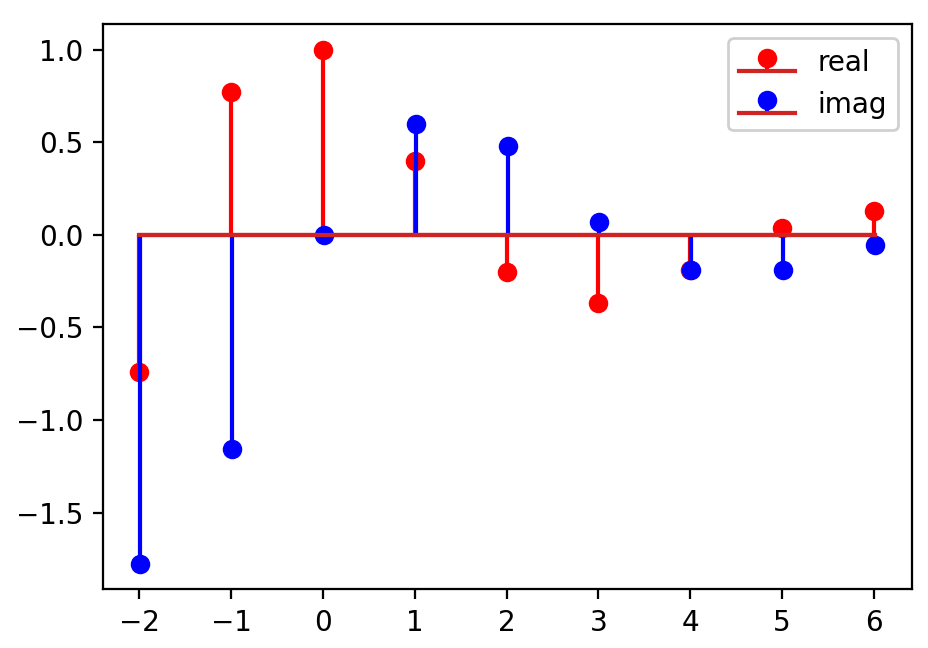
\includegraphics[width=\textwidth]{code/complex_exp.png}
    \end{minipage}
    \codecaption{code/complex_exp.py}{Berechnung und Darstellung eines komplexen exponentiellen Signals}\label{py:complex_exp}
\end{listing}
%
\subsubsection{Energie Diskreter Signale}

Oft ist es interessant zu bemessen, wie viel Energie in einem Signal vorhanden ist.
F"ur eine physikalisch korrekte Bemessung dieser Energie, m"usste man das Signal zwar mit Einheiten versehen, aber diese ergeben nur einen entsprechenden Proportionalit"atsfaktor.
Hierzu betrachten wir
\begin{equation}\label{eq:disc_sig_energy}
    E(x[\cdot]) 
        = \Sum{n \in \Z}{}{\Abs{x[n]}^2} 
        = \Sum{n \in \Z}{}{x[n]^\ast \cdot x[n]}.
\end{equation}
Wenn gilt $E(x[\cdot]) < \infty$, dann sprechen wir erstaunlicherweise von einem Signal endlicher Energie.

Es ist nun interessant sich eine Menge $\mathcal{E}$ zu definieren, die alle Signale enth"alt, welche endliche Energie besitzen, also 
\[
    \mathcal{E} = \{x : \Z \rightarrow \C \Text{mit} E(x[\cdot]) < \infty\}.
\]
Man kann sich nun "uberlegen, dass
\[
E(\alpha x[\cdot] + \beta y[\cdot]) 
    \leqslant E(\alpha x[\cdot]) + E(\beta y[\cdot])
    = \alpha^2 E(x[\cdot]) + \beta^2 E(y[\cdot]) 
    < \infty 
\]
gelten muss, falls $E(x[\cdot]),E(y[\cdot]) < \infty$. 
Das hei"st, dass Linearkombinationen von Signalen mit endlicher Energie wieder ein Signal mit endlicher Energie ergeben.
Das hei"st, dass die Signale endlicher Energie bilden einen \emph{Unterraum}.
Wir k"onnen noch einen Schritt weiter gehen und wie in \eqref{eq:dtft_inner_prod} die Summe in \eqref{eq:disc_sig_energy} als Skalarprodukt auffassen.

Definieren wir f"ur zwei Signale endlicher Energie die Abbildung $\ScPr{\cdot}{\cdot} : \mathcal{E} \times \mathcal{E} \rightarrow \C$ als
\begin{equation}\label{eq:disc_inner_prod}
    (x[\cdot], y[\cdot]) 
        \mapsto \ScPr{x[\cdot]}{y[\cdot]}
        = \Sum{n \in \Z}{}{x[n]^\ast \cdot y[n]},
\end{equation}
dann kann man sich "uberlegen, dass dies die Bedingungen an ein \emph{Skalarprodukt} erf"ullt.
Beispielsweise kann man nachrechnen, dass die unendliche Summe in \eqref{eq:disc_inner_prod} immer endlich ist, falls $x[\cdot], y[\cdot] \in \mathcal{E}$, da
\[
\Abs{\ScPr{x[\cdot]}{y[\cdot]}} \leqslant E(x[\cdot]) \cdot E(y[\cdot]) < \infty
\]
Nun kann man aber auch $E$ durch
\[
E(x[\cdot]) = \ScPr{x[\cdot]}{x[\cdot]}
\] 
ausdr"ucken.

\begin{Bsp}
Betrachten wir $x[n] = a^n \cdot u[n]$ f"ur $a = r \exp{\jmath \theta} \in \C$.
Dann berechnet sich $E(x[\cdot])$ durch
\[
E(x[\cdot]) 
    = \Sum{n \geqslant 0}{}{\Abs{a^n}^2} 
    = \Sum{n \geqslant 0}{}{\left(r^2\right)^n}.
\]
Ist nun $r \geqslant 1$, dann $E(x[\cdot]) = \infty$, falls aber $r < 1$, dann ergibt sich aus der geometrischen Reihe, dass
\[
    E(x[\cdot]) = \frac{1}{1 - r^2}
\]
gilt.
Das hei"st auch, dass das Heavy-Side-Signal $u[\cdot]$ keine endliche Energie besitzt.
\end{Bsp}
%
\subsubsection{Periodische Signale}
%
Gilt f\"ur ein Signal $x[\cdot]$, dass $x[n + N] = x[n]$ f"ur ein $N \in \N$ und \emph{alle} $n \in \Z$, so nennt man $x[\cdot]$ periodisch mit Periodenl"ange/Periode $N$, oder kurz $N$-periodisch, siehe beispielsweise \Cref{eq:disc_harms_comp}.
Falls $x[\cdot]$ nun $N$-periodisch ist, dann ist $x[\cdot]$ auch $kN$-periodisch, falls $k \in \N$.
Das hei"st, dass es sinnvoller ist, das \emph{kleinste} $N \in \N$ zu betrachten, sodass $x[\cdot]$ dann $N$-periodisch ist. 
Man nennt $N$ dann Fundamentalperiode.
Falls solch ein $N$ nicht existiert, dann nennt man $x[\cdot]$ aperiodisch, oder nicht-periodisch.
Falls $x[\cdot] \neq 0$, dann gilt f"ur periodische Signale, dass $E(x[\cdot]) = \infty$.
Beispielsweise haben wir bereits in \Cref{sec:sample_harm} gesehen, dass
\[
x[n] = \exp(\jmath 2 \pi f)
\]
periodisch mit Periode $N$ ist, falls $f = k/N$, also eine rationale Zahl ist.
%
\subsubsection{Symmetrie von Signalen}
%
Gilt f"ur ein Signal $x[n] = x[-n]$, dann nennt man es \emph{symmetrisch} bzw.~\emph{gerade}.
Gilt andererseits $x[n] = -x[-n]$, so nennt man es \emph{anti-symmetrisch} bzw.~\emph{ungerade}.

Ist ein beliebiges Signal $x[\cdot]$ gegeben, so kann man
\[
    x_g[n] = \frac 12 \left(x[n] + x[-n]\right)
    \Text{und}
    x_u[n] = \frac 12 \left(x[n] - x[-n]\right)
\]
definieren.
Dann ist $x_g[\cdot]$ gerade und falls $x[\cdot]$ bereits gerade ist, so gilt $x[\cdot] = x_e[\cdot]$.
Genauso ist $x_u[\cdot]$ ungerade und falls $x[\cdot]$ bereits ungerade ist, so gilt $x[\cdot] = x_u[\cdot]$.
Au"serdem gilt
\[
x[n] = x_g[n] + x_u[n].
\]
Wir haben das Signal $x[\cdot]$ also in einen geraden und einen ungeraden Teil zerlegt.
Dies ist manchmal sinnvoll, wenn man solch ein Signal linear transformiert und wei"s, dass die lineare Transformation f"ur gerade oder ungerade Signale gewisse Eigenschaften hat.
Wie man an \Cref{py:even_odd} gut sehen kann, muss gelten $x_u[0] =0$, da $x_u[0] = x[0] - x[0] = 0$ und $x_e[0] = x[0]$, da $2 x_e[0] = x[0] + x[0]$.
%
\begin{listing}
    \noindent
    \begin{minipage}{0.49\textwidth}
        \strut\vspace*{-\baselineskip}\newline
        \inputminted[firstline=4]{python3}{code/even_odd.py}
    \end{minipage}%
    \begin{minipage}{0.49\textwidth}
        \strut\vspace*{-\baselineskip}\newline
        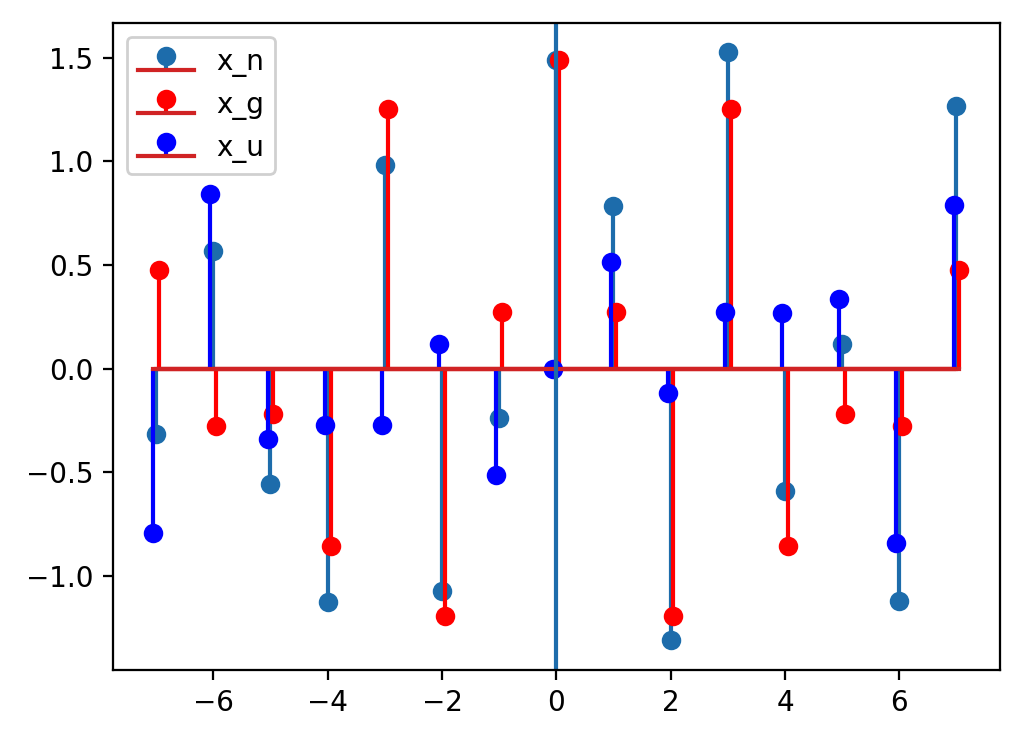
\includegraphics[width=\textwidth]{code/even_odd.png}
    \end{minipage}
    \codecaption{code/even_odd.py}{Zerlegung eines Signals in seinen geraden und ungeraden Anteil.}\label{py:even_odd}
\end{listing}
%
\subsection{Diskrete Systeme}
%
%
Nachdem wir uns nun ein wenig mit diskreten Signalen vertraut gemacht haben, sind wir in der Lage und mit diskreten Systemen zu befassen.
Ganz allgemein kann man fast jeden Prozess, an dessen Anfang ein diskretes Signal steht und dessen Ergebnis wiederum ein diskretes Signal ist, als ein diskretes System auffassen.
Sobald man dieses System nun einmal vorliegen hat, will man Techniken und Werkzeugen entwickeln, wie man dieses System systematisch untersuchen kann -- eine Systematik der Systeme.

Ein System $\mathcal{T}$ wird mathematisch als Abbildung eines (Eingabe-)Signals $x[\cdot]$ auf ein anderes (Ausgabesignal) $y[\cdot]$ aufgefasst. Wir schreiben daf"ur dann
%
\begin{equation}\label{eq:gen_disc_sys}
    x[\cdot] \mapsto \mathcal{T}(x[\cdot])[\cdot] = y[\cdot].
\end{equation}
%
Das System $\mathcal{T}$ bildet also die Paare $(x[\cdot], \mathcal{T}(x[\cdot])) = (x[\cdot], y[\cdot])$.

Betrachten wir folgendes
\begin{Bsp}\label{ex:simple_sys}
    Gegeben sei das Eingabesignal
    \[
    x[n] = \begin{cases}
        \Abs{n}, \Text{falls} -3 \leqslant n \leqslant +3, \\
        0 \Text{sonst.}
    \end{cases}
    \]
    Wir sind nun an den Werten der Ausgabesignals $y[\cdot]$ interessiert, f"ur
    \begin{enumerate}[a)]
        \item das Einheitssystem $y[n] = x[n]$,
        \item das Einheitsdelay-System $y[n] = x[n-1]$,
        \item das Einheitsadvance-System $y[n] = x[n+1]$
    \end{enumerate}
    interessiert.
\end{Bsp}
Diese Systeme waren noch ein wenig simpel und man ist vielleicht noch nicht "uberzeugt, dass eine genauere Analyse von diskreten Systemen notwendig sein sollte.
Dies liegt vor allem daran, dass die Systeme in \Cref{ex:simple_sys} nur \q{lokal} gearbeitet haben, da Werte $y[n]$ nur von Werten $x[n-1]$, $x[n]$ und $x[n+1]$ abh"angen.

Betrachten wir wiederum die Mandelbrot-Iteration, aber diesmal als System
\[
    y[n+1] = y[n]^2 + x[n]
\]
f"ur verschiedene Eingangssignale $x[n] = c \in \C$ mit $y[0] = 0$.
Wir sind nun an solchen $c$ interessiert f"ur welche das System divergiert, also $\Abs{y[n]} > 2$ ab einem gewissen $n$.
Wir wollen aber solche $c$ finden, f"ur welche wir in einem gewissen Bereich $n \in [n_{\rm low}, n_{\rm hgh}]$ divergieren.
Das in \Cref{py:buddhabrot} gezeigte Beispiel ist hierbei am anderen Ende des Komplexit"atsspektrums, da man bei diesem System eher von einem \q{chaotischen} System sprechen sollte. 
Kleine Ver"anderungen an $x[n] = c$ haben gro"sen Einfluss auf das Divergenzverhalten der Folge $y[n]$\footnote{\url{https://erleuchtet.org/2010/07/ridiculously-large-buddhabrot.html}}.
\begin{listing}
    \noindent
    \begin{minipage}{0.49\textwidth}
        \strut\vspace*{-\baselineskip}\newline
        \inputminted[firstline=5,lastline=26]{python3}{code/buddhabrot.py}
    \end{minipage}%
    \begin{minipage}{0.49\textwidth}
        \strut\vspace*{-\baselineskip}\newline
        \inputminted[firstline=29,lastline=53]{python3}{code/buddhabrot.py}
    \end{minipage}

    \begin{center}
        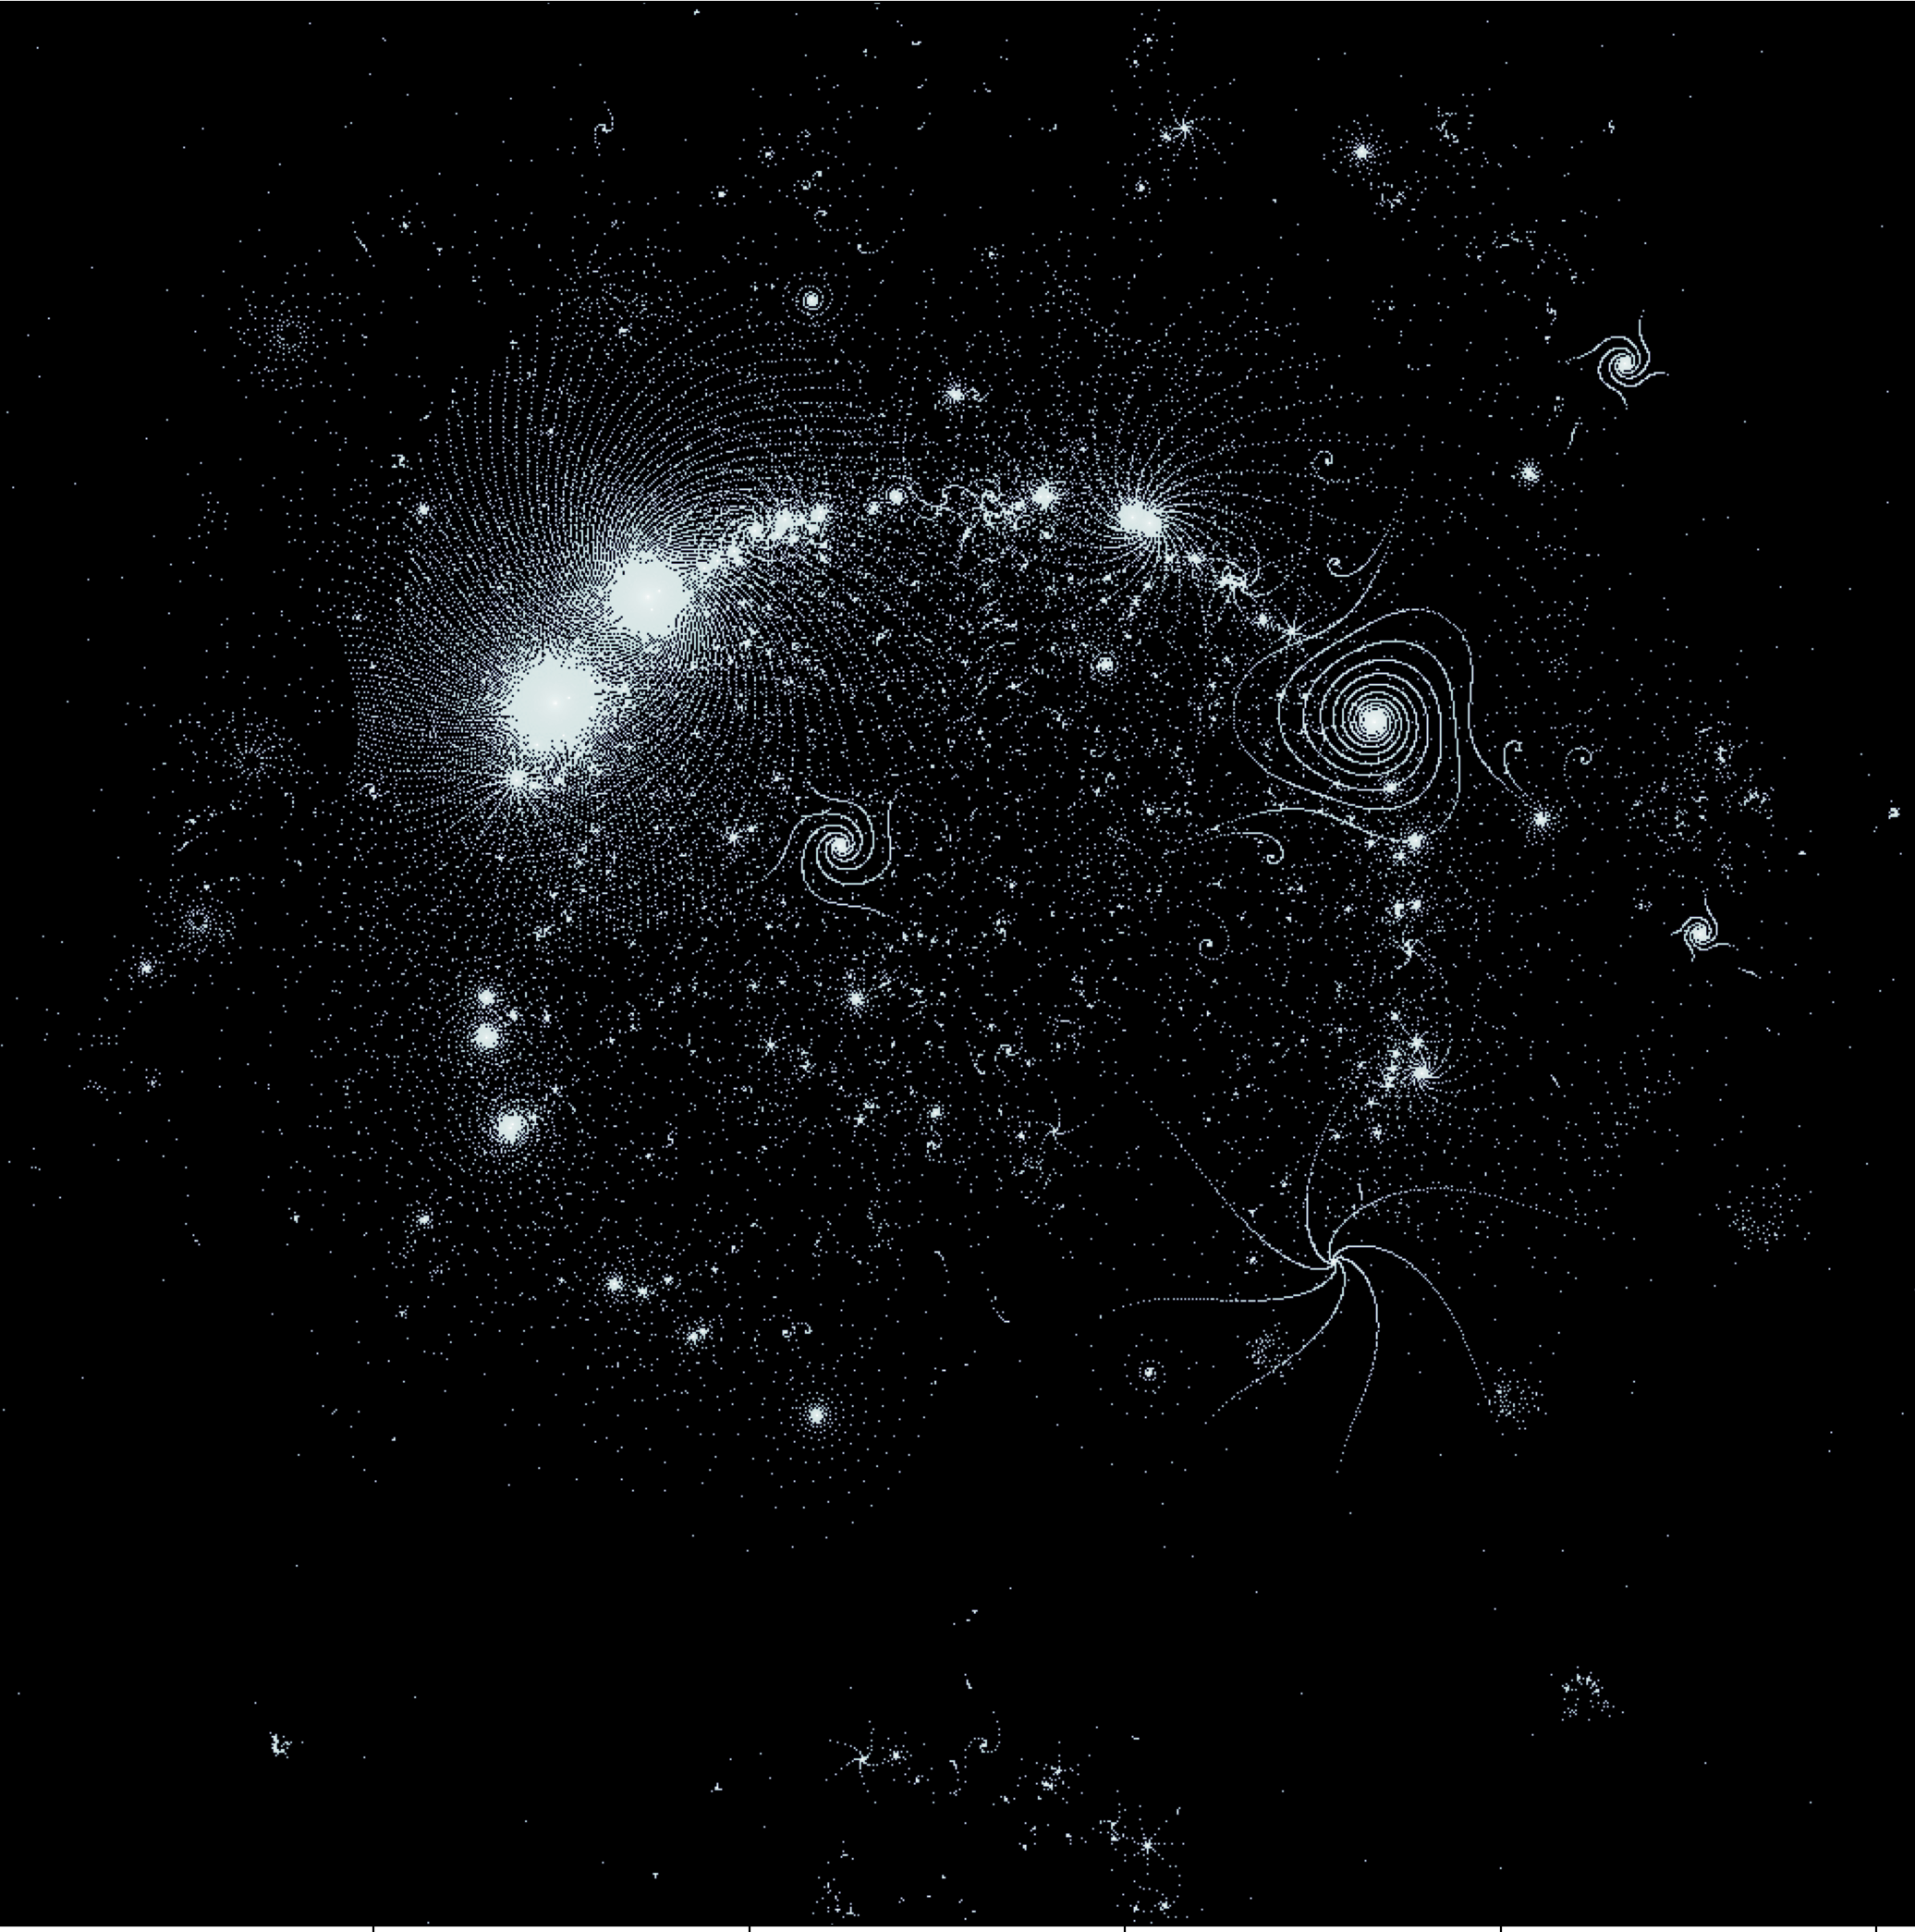
\includegraphics[width=0.55\textwidth]{code/buddhabrot.png}
    \end{center}
    \codecaption{code/buddhabrot.py}{Sp"at divergierende Orbits der Mandelbrot-Iteration.}\label{py:buddhabrot}
\end{listing}

Um zu sehen, wie Systeme von ihrem Anfangszustand abh"angen k"onnen, wollen hierf"ur ein etwas einfacheres Beispiel betrachten. 
Gegeben ist das System
\[
y[n] = \Sum{k=-\infty}{n}{x[k]}.
\]
Wir sehen hier, dass es f"ur die Berechnung von $y[n]$ nicht ausreicht, den Zustand des Eingangs zum Zeitpunkt $n$, also $x[n]$ zu kennen.
Schlie"slich m"ussen wir die gesamte Vergangenheit von $x[\cdot]$ bis zum Zeitpunkt $n$ in die Berechnung einflie"sen lassen.
Wir k"onnen das System aber umschreiben in 
\[
y[n] = \Sum{k=-\infty}{n-1}{x[k]} + x[n] = y[n-1] + x[n],
\]
wobei wir nun auch sehen, warum dieses System \emph{Akkumulator} genannt wird, da $y[\cdot]$ im Prinzip die Werte von $x[\cdot]$ \q{aufsammelt}.

Stellen wir uns nun vor, dass wir dieses System modellieren/simulieren wollen f"ur $n \leqslant n_0$, so ben"otigen wir entweder die Werte $x[n]$ f"ur $n < n_0$, oder die sogenannte \emph{Anfangsbedingung} $y[n_0] = y_0$.
Dies erinnert an das L"osen einer Differentialgleichung
\[
\dot{y}(t) = x(t),
\]
wonach dann gilt, dass
\[
y(t) = \Int{-\infty}{t}{x(s)}{s} 
\Text{oder}
y(t) = y_0 + \Int{t_0}{t}{x(s)}{s},
\]
damit $y(t_0) = y_0$.
Ein Beispiel f"ur die Wirkung von einem Akkumulator ist in \Cref{py:accumulator} gegeben. 
Man sieht sehr gut, welchen Einfluss die Anfangsbedingung auf $x_2[\cdot]$ hat, da dies den Grenzwert $\lim_{n \rightarrow \infty} y[n]$ ma"sgeblich beeinflusst.
Falls gilt, dass $y_0 = 0$, so spricht man vom Ruhezustand, beziehungsweise dem Nullzustand in dem sich das System zum Zeitpunkt $n = n_0$ befindet.
%
\begin{listing}
    \noindent
    \begin{minipage}{0.49\textwidth}
        \strut\vspace*{-\baselineskip}\newline
        \inputminted[firstline=4,lastline=18]{python3}{code/accumulator.py}
    \end{minipage}%
    \begin{minipage}{0.49\textwidth}
        \strut\vspace*{-\baselineskip}\newline
        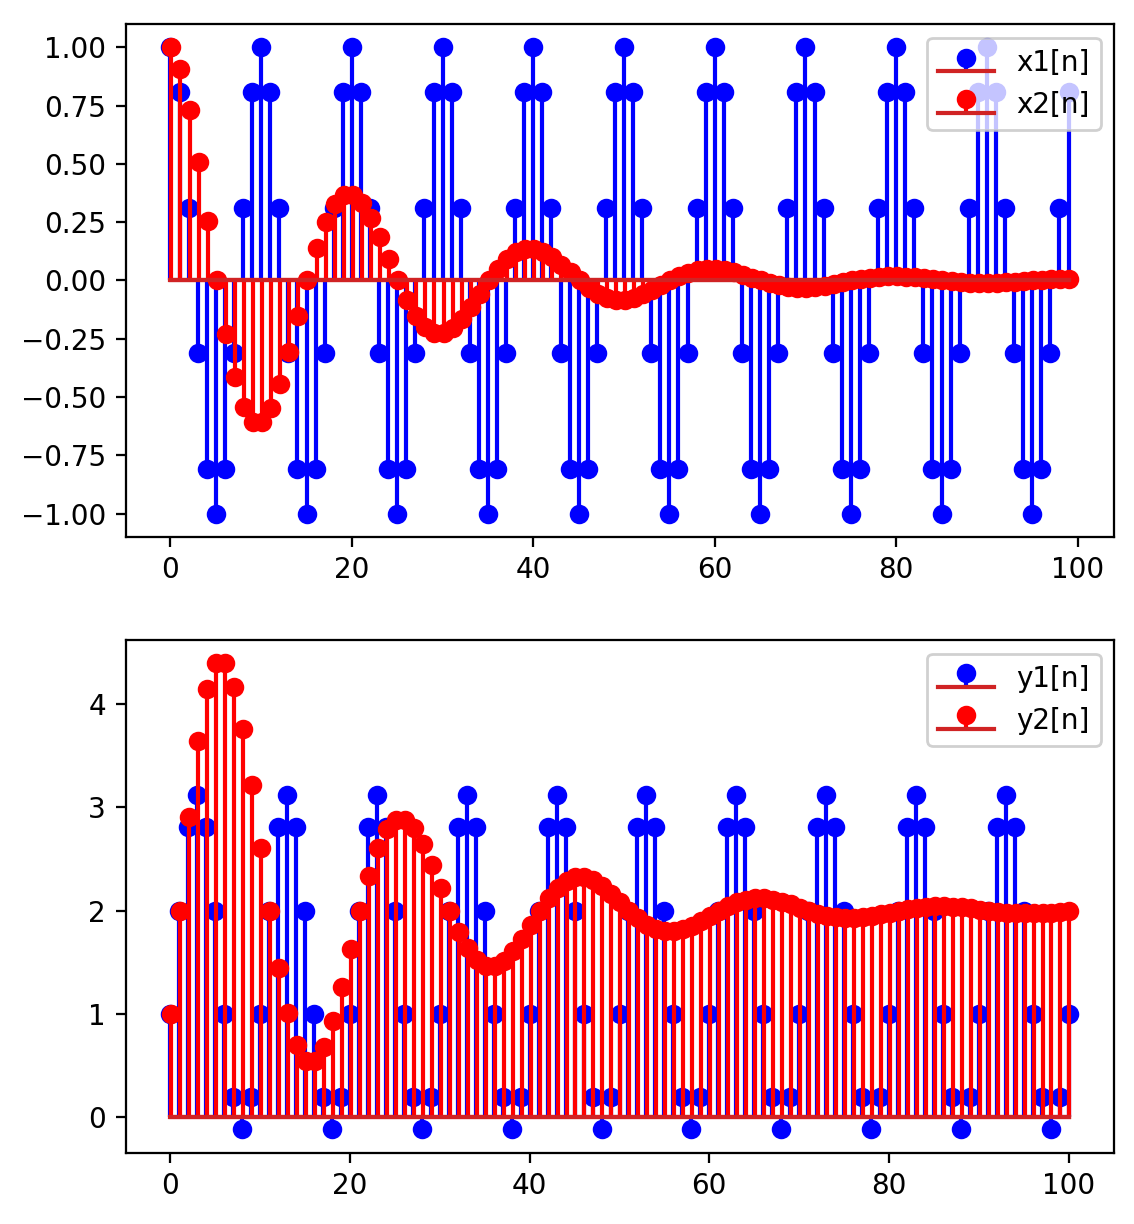
\includegraphics[width=\textwidth]{code/accumulator.png}
    \end{minipage}%
    \codecaption{code/accumulator.py}{Akkumulator f"ur zwei verschiedene Eingangsignale.}\label{py:accumulator}
\end{listing}

\paragraph{Statisch vs. Dynamisch}
Man kann Systeme nun auf verschiedene Arten klassifizieren.
Beispielsweise nennen wir Systeme \emph{statisch}, wenn der Wert $y[n]$ nur von $x[n]$ abh"angt, aber nicht von vergangenen oder gar zuk"unftigen Werten (entweder von $y[\cdot]$ oder $x[\cdot]$).
Die Systeme
\[
y[n] = a x[n], \Text{oder} y[n] = \sqrt{x[n]} + x^4[n]
\]
sind statisch.
H"angt nun $y[n]$ von seiner eigenen Vergangenheit oder der von $x[n]$ ab, so nennen wir diese Systeme dynamisch, oder Systeme mit Ged"achtnis.
Die Systeme
\[
y[n] = x[n] + a x[n-1] \Text{,} y[n] = \Sum{k=0}{N}{x[n-k]}
\]
sind dynamisch und haben jeweils Ged"achtnis der L"ange $g = 1$, beziehungsweise $g = N-1$.
Man sieht bereits an \Cref{py:accumulator}, dass dynamische System im Allgemeinen interessanter sein werden.

\paragraph{Kausal vs. Akausal} 
H"angen die Werte $y[n]$ nur von $x[n], x[n-1], \dots$ ab, also nicht auch von $x[n+1], x[n+1], \dots$, so nennen wir das System kausal.
Intuitiv bedeutet dies die intuitiv bekannte Kausalit"at in dem Sinne, dass nur die Zeitliche Vergangenheit notwendig ist, um den aktuellen Zustand des Systems zu bestimmen.
Ist die nicht gegeben, so nennt man das System \emph{akausal} oder \emph{nicht-kausal}.

Was die Realisierung von akausalen Systemen angeht, wird es nicht m"oglich sein, diese in Echtzeit umzusetzen, da man diese nur mit einer Verz"ogerung, oder gar nicht f"ur sequentiell verf"ugbares $x[\cdot]$ implementieren kann.
Sind die Werte $x[n]$ jedoch beispielsweise durch Messung oder Simulation entstanden und \q{offline} verf"ugbar, so k"onnen solche Systeme durchaus angewandt werden und n"utzlich sein.

\paragraph{Stabil vs. Instabil} Eine der zentralen Eigenschaften, die auch bei analogen Systemen eine Rolle spielt ist Stabilit"at.
Zwar hat man normalerweise bereits einen intuitiven Begriff f"ur Stabilit"t im Sinn, doch formal gibt es hiervon verschiedene Auspr"agungen.
Wir beschr"anken uns auf die Version der \gls{bibo}-Stabilit"at, welche fordert, dass f"ur beschr"anktes Eingangssignal $x[\cdot]$ der Ausgang $y[\cdot]$ ebenfalls beschr"ankt bleibt.
Formal fordern wir also, dass falls
\[
\Abs{x[n]} \leqslant M_x \Text{f"ur alle} n \in \Z
\]
f"ur eine Konstante $M_x \in \R$ gilt, dann auch 
\[
\Abs{y[n]} \leqslant M_y \Text{f"ur alle} n \in \Z
\]
gelten muss. 
Man sieht, dass $M_x$ und $M_y$ an $x[\cdot]$ und $y[\cdot]$ gebunden sind, also keine \q{universellen} Konstanten sind.
Andersherum reicht es also f"ur Instabilt"at nur \emph{ein} beschr"anktes Eingangssignal $x[\cdot]$ konstruiert werden muss, f"ur welches $y[\cdot]$ nicht beschr"ankt bleibt.
Betrachten wir folgendes
\begin{Exm}
Gegeben sei
\[
y[n] = C \cdot y[n-1]^2 + x[n]
\]
und wir nutzen als Eingang den Einheitssto"s $x[\cdot] = C \delta[\cdot]$, welcher beschr"ankt ist, mit $M_x = \Abs{C}$ f"ur $C \in \R$.
Doch dieser produziert f"ur $y[n] = 0$ f"ur $n \leqslant -1$ die Folge
\[
y[n] = \{0, \Start{C}, C^2, C^4, \dots, C^{2n}\},
\]
welche f"ur $\Abs{C} > 1$ gegen $\infty$ divergiert.
\end{Exm}

\paragraph{Zeitvariant vs. Zeitinvariant} Systeme deren Eingabe-Ausgabe-Verhalten nicht zeitlich konstant ist, nennt man \emph{zeitvariant}.
Systeme, die f"ur zeit verz"ogerte Eingaben, die um den gleichen Zeitraum verz"ogerte Ausgaben produzieren, nennt man \emph{zeitinvariant}, siehe \Cref{exm:cont_lit}.
Formal fordern wir f"ur Zeitinvarianz, dass wenn f"ur beliebige Eingabe $x[\cdot]$
\[
x[\cdot] \overset{\mathcal{T}}{\rightarrow} y[\cdot]
\]
gilt, dass dann f"ur jedes $k \in Z$ auch gilt, dass
\[
x[\cdot -k] \overset{\mathcal{T}}{\rightarrow} y[\cdot - k]
\]
erf"ullt ist.
In der Schreibweise von \eqref{eq:gen_disc_sys} hei"st dies, dass f"ur 
\[
    y[n] = \mathcal{T}(x[\cdot])[n]
\]
auch gelten muss, dass
\[
    y[n - k] = \mathcal{T}(x[\cdot - k])[n]
\]
und zwar f"ur alle $x[\cdot]$ und $k$.

Was erst einmal relativ abstrakt daherkommt, ist eigentlich eine sehr intuitive Sache. 
Wenn wir beispielsweise an ein Audiointerface denken, so h"atten wir schon gerne, dass es egal ist, zu welchem Zeitpunkt jemand ins Mikrophon singt -- unabh"angig vom Zeitpunkt sollte die Aufnahme \q{gleich klingen}.
Das System, welches die Aufnahme und eventuelle Audioverarbeitung realisiert, sollte keine zeitlichen Ver"anderungen zeigen.
Auch in der umgekehrten Richtung, beim Abspielen von Ton, sollte es irrelevant sein, zu welchem Zeitpunkt man ein gewisses St"uck h"oren m"ochte -- das H"orerlebnis sollte davon nicht beeinflusst sein.

Im Grunde ist Zeitinvarianz also etwas, das wir normalerweise von einem System \q{erwarten} und nicht untersuchen wollen.

\paragraph{Linear vs. Nicht-Linear} Kommen wir zum Schluss dieser Klassifikationen zu einer der wichtigsten Unterscheidungen.
Ein System, das f"ur Eing"ange $x_1[\cdot]$ und $x_2[\cdot]$ die Antworten
\[
    y_1[n] = \mathcal{T}(x_1[\cdot])[n]
    \Text{und}
    y_2[n] = \mathcal{T}(x_2[\cdot])[n]
\]
produziert, nennen wir \emph{linear}, falls die Antwort des Systems auf den Eingang
\[
    x[\cdot] = a_1 x_1[\cdot] + a_2 x_2[\cdot]
\]
sich durch
\[
    y[n]
        = \mathcal{T}(x[\cdot])[n] 
        = \mathcal{T}(a_1 x_1[\cdot] + a_2 x_2[\cdot])[n] 
        = a_1 \mathcal{T}(x_1[\cdot])[n] 
            + a_2 \mathcal{T}(x_2[\cdot])[n] 
\]
ausdr"ucken l"asst.
%
\begin{figure}
    \centering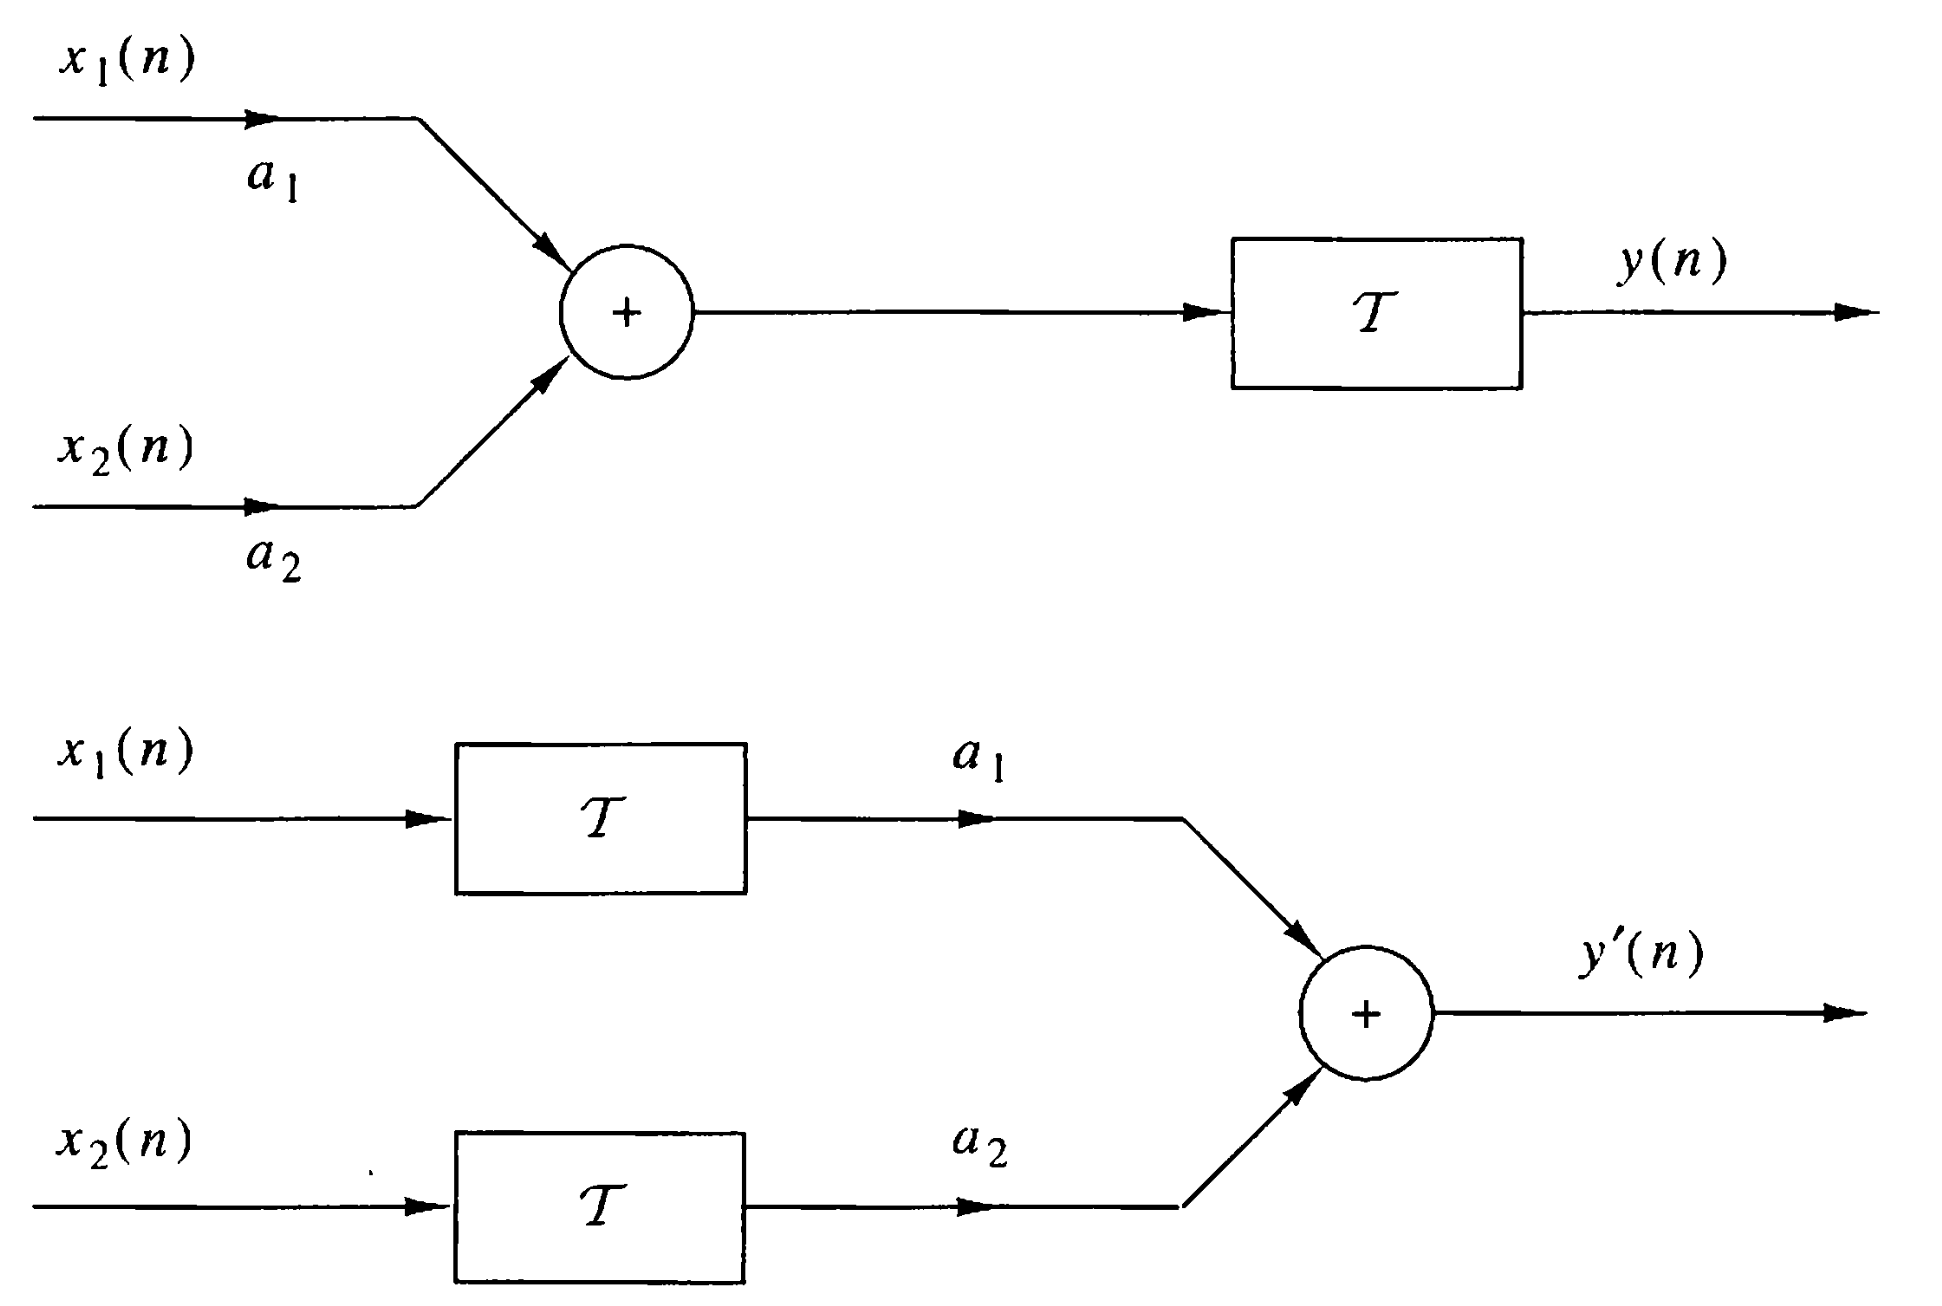
\includegraphics[width=0.6\textwidth]{img/disc_sys/linear_sys.png}
    \caption{zeigt zwei verschiedene systemtheoretische Interpretation von linearen Systemen. Quelle: \cite{proakis2013}}\label{img:disc_sys:linear_sys}
\end{figure}
%

\Cref{img:disc_sys:linear_sys} zeigt die beiden m"oglichen Interpretationen dieser Eigenschaft.
Man kann sich also vorstellen, dass die Eing"ange \emph{erst} skaliert und addiert werden und dann das System durchlaufen, oder man prozessiert beide Eing"ange durch $\mathcal{T}$ und skaliert und addiert die \emph{Ausg"ange nachdem} das System im Grund \q{zweifach} angewandt wurde.

Anders gesagt \q{passen} lineare Systeme genau zu der linearen Struktur von Signalen, wenn wir sie als Vektoren in einem Vektorraum auffassen.
Als Konsequenz ergibt sich, dass sich lineare Systeme deutlich einfacher analysieren lassen, weil wir Werkzeuge der linearen Algebra benutzen k"onnen.
Diese Eigenschaft ist so attraktiv, dass man oft versucht nichtlineare Systeme durch geeignete lineare System zu approximieren (Bsp: Pendel $\sin(x) \approx x$).
Man nimmt also Fehler in der Analyse in Kauf, ist damit aber immerhin in der Lage "uberhaupt Aussagen treffen zu k"onnen.
%
%
\subsection{Diskrete \texorpdfstring{\acrshort{lti}}{LTI}-Systeme}\label{sec:disc_lti}
%

Wir schr"anken nun die Menge der Systeme ein, die wir betrachten wollen, indem wir fordern, dass das System $\mathcal{T}$ gleichzeitig linear und zeitinvariant ist.
Das hei"st, es gilt einerseits, dass ein Eingang $x[\cdot]$ zum System $\mathcal{T}$ mit Ausgang $y[\cdot]$ bei Verz"ogerung zu $x[\cdot - k]$ den entsprechend verz"ogerten Ausgang $y[\cdot - k]$ zur Folge hat.
Gleichzeitig kann der Ausgang des Systems $\mathcal{T}$ f"ur Eingange, die lineare Superpositionen sind als lineare Superposition von den entsprechenden Ausg"angen ausgedr"uckt werden, siehe \Cref{img:disc_sys:linear_sys}.

\subsubsection{Faltungsformel}

Wir wollen die Struktur von \gls{lti}-Systemen ausnutzen, um eine allgemeine und einfache Formel f"ur das Eingangs-Ausgangsverhalten von jenen angeben zu k"onnen.
Als Erstes verallgemeinern wir hierzu \Cref{img:disc_sys:linear_sys} zu beliebigen, aber endlichen Summen, also gegeben ist ein Eingang $x[\cdot]$ der Form
\begin{equation}\label{eq:lti_sys:input}
    x[n] = \Sum{k=1}{K}{a_k \cdot x_k[n]},
\end{equation}

wobei wir wissen, wie die Ausg"ange von jedem $x_k[\cdot]$ zu berechnen sind, also
\[
    y_k[n] = (\mathcal{T}x_k[\cdot])[n].
\]
Dann wissen wir wegen der Linearit"at und \eqref{eq:lti_sys:input}, dass
\begin{equation}\label{eq:lti_sys:superpos}
    y[n] 
        = \left[\mathcal{T}\left(
            \Sum{k=1}{K}{a_k \cdot x_k[\cdot]}
        \right)\right][n] 
        = \Sum{k=1}{K}{
            a_k (\mathcal{T}x_k[\cdot])[n]
        }
        = \Sum{k=1}{K}{
            a_k y_k[n]
        }
\end{equation}
gelten muss.
Es lohnt sich einige Zeit "uber diese Sache zu meditieren und es gibt verschiedene Interpretationen.
\begin{itemize}
    \item Wie bereits erw"ahnt passt dies zur linearen Struktur des Systems $\mathcal{T}$.
    \item Ist ein Eingangssignal aus anderen Signalen zusammengesetzt, dann setzt sich die Reaktion des Systems auf dieses zusammengesetzte Signal aus den Reaktionen auf die Signalbausteine zusammen. 
    Wichtig ist hierbei, dass die Art der Zusammensetzung sich nicht "andert. Die $a_k$ in \eqref{eq:lti_sys:superpos} sind die gleichen, wie in \eqref{eq:lti_sys:input}.
\end{itemize}

Wir wollen nun einen Schritt weiter gehen und eine Menge von $x_k[\cdot]$ angeben, die es erlauben \emph{alle} m"oglichen Signale darzustellen.
Dazu betrachten wir, was geschieht, wenn wir den Einheitssto"s $\delta[\cdot]$ mit einem beliebigen Signal multiplizieren.
Wir rechnen demzufolge f"ur ein beliebiges Signal
\[
x[n] \cdot \delta[n] = \begin{cases}
    x[0] \Text{f"ur} n = 0 \\
    0 \Text{sonst.}
\end{cases}
\]
Wenn wir nun die Einheitsst"o"se verschieben um $k \in \Z$ erhalten wir
\[
    x[n] \cdot \delta[n-k] = \begin{cases}
        x[k] \Text{f"ur} n = k \\
        0 \Text{sonst.}
    \end{cases}
\]
Im Grunde \q{pickt} $\delta[\cdot-k]$ bei Multiplikation den Wert von $x[\cdot]$ an der Stelle $k$ heraus.
Deshalb k"onnen wir nun schreiben
\begin{equation}
    x[n] = \Sum{k \in \Z}{}{
        x[k] \cdot \delta[n-k],
    }
\end{equation}
was nach Definition von $x_k[\cdot] = \delta[\cdot - k]$ genau die Form von \eqref{eq:lti_sys:input} mit $a_k = x[k]$ annimmt.
Die Kernbeobachtung ist nun, dass jedes $x_k[\cdot]$ eine verschobene Kopie von $\delta[\cdot]$ ist. 
Das hei"st, dass wir nun die \gls{lti}-Eigenschaft ausnutzen k"onnen, weil \eqref{eq:lti_sys:superpos} impliziert, dass wir nur $(\mathcal{T}\delta[\cdot])[\cdot]$ berechnen m"ussen und $(\mathcal{T}\delta[\cdot - k])[\cdot]$ sich als $(\mathcal{T}\delta[\cdot])[\cdot - k]$ ergibt.

Wir geben dem Kind nun einen Namen, also definieren wir $h: \Z \rightarrow \C$ als die Antwort des Systems $\mathcal{T}$ auf den Eingang $\delta[\cdot]$, also
\begin{equation}\label{eq:lti_sys:ir}
    h[n] = (\mathcal{T} \delta[\cdot])[n].
\end{equation}
Man nennt $h[\cdot]$ die \emph{Impulsantwort} des Systems.
Dann k"onnen wir also mit \eqref{eq:lti_sys:superpos} folgern, dass
\begin{equation}\label{eq:lti_sys:conv}
    y[n] 
        = (\mathcal{T} x[\cdot])[n] 
        = \Sum{k \in \Z}{}{
            x[k] h[n-k]
        }
\end{equation}
gelten muss.

Das hei"st, dass sich die Antwort $y[\cdot]$ eines diskreten \gls{lti}-Systems aus der \emph{Faltung} des Einganges $x[\cdot]$ mit der Impulsantwort $h[\cdot]$ ergibt.
Wir schreiben in Kurzform
\[
y[n] = (x \ast h)[n] = (h \ast x)[n].
\]
Es wird sich zeigen, dass sich viele Eigenschaften des Systems $\mathcal{T}$ an oft einfacher zu pr"ufenden Eigenschaften der Impulsantwort $h[\cdot]$ ergeben.
Das hei"st, dass $h[\cdot]$ in gewisser Weise das System $\mathcal{T}$ repr"asentiert.
%
\begin{listing}
    \noindent
    \begin{minipage}{0.49\textwidth}
        \strut\vspace*{-\baselineskip}\newline
        \inputminted[firstline=10,lastline=22]{python3}{code/moving_average.py}
    \end{minipage}%
    \begin{minipage}{0.49\textwidth}
        \strut\vspace*{-\baselineskip}\newline
        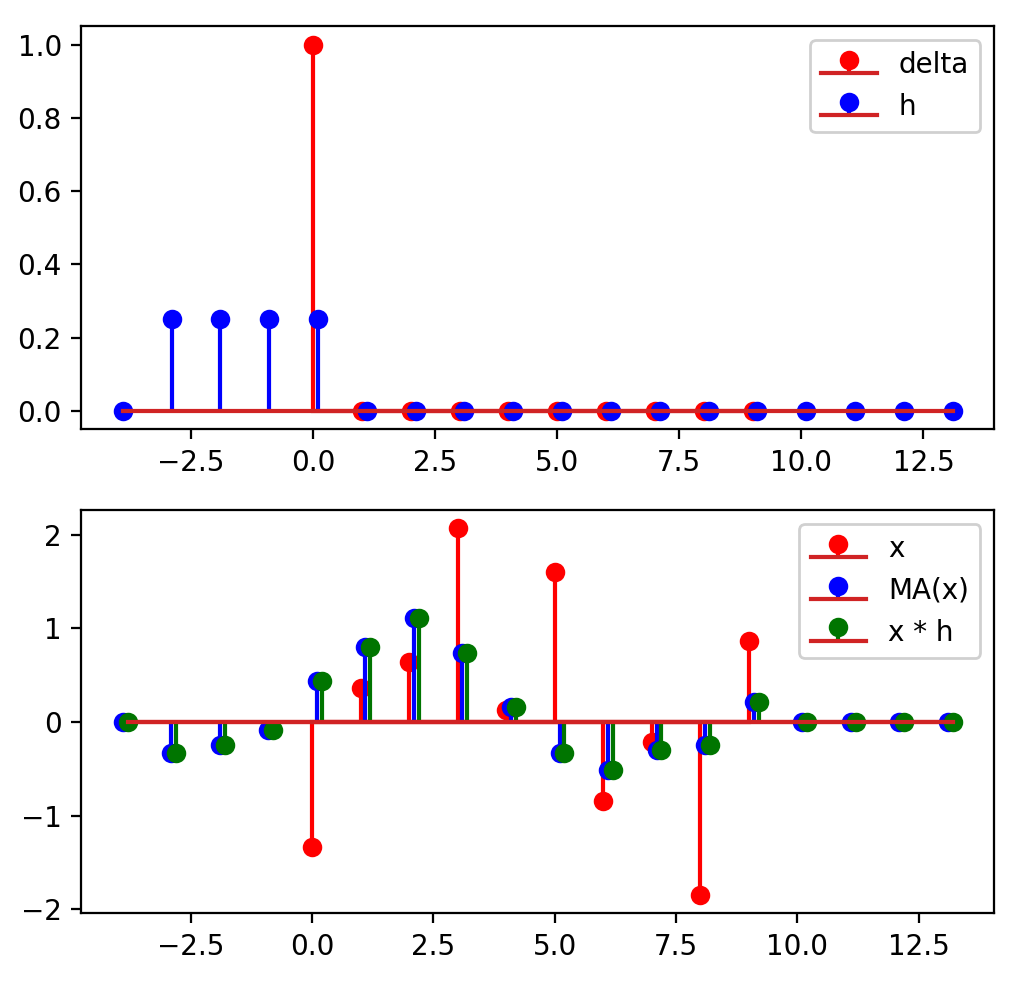
\includegraphics[width=\textwidth]{code/moving_average.png}
    \end{minipage}
    \codecaption{dsv/code/moving_average.py}{Gleitendes Mittel mit L"ange $\ell=4$. Wir vergleichen die direkte Berechnung mit der Berechnung "uber die Faltung}\label{py:moving_average}
\end{listing}

In \Cref{py:moving_average} zeigen wir das Verhalten eines gleitenden Mittelwertes (\emph{moving average}), welches sich durch
\[
y[n] = \frac{1}{\ell} \Sum{k=0}{k=\ell}{x[n-k]}
\]
ergibt.
Man sieht sch"on, dass durch das Mitteln die (in diesem Fall) zuf"allige Eingabe-Sequenz am Ausgang gegl"attet erscheint.
Wichtig bei diesem Beispiel ist die Tatsache, dass wir direkt einsehen, dass Anwendung der direkten Formel f"ur das gleitende Mittel aus eine Eingabe $x[\cdot]$ denselben Effekt hat, wie die Faltung mit $h[\cdot]$, das sich aus der Anwendung der Mittelung auf $\delta[\cdot]$ ergibt.

Es lohnt sich, sich einige Eigenschaften der Faltung zu merken. 
Diese sind:
\begin{itemize}
    \item Bi-Linearit"at: Es gilt $(a_1 x_1[\cdot] + a_2 x_2[\cdot]) \ast h[\cdot] = a_1 (x_1 \ast h)[\cdot] + a_2 (x_2 \ast h)[\cdot]$. 
    Dies ist die \q{normale} Linearit"at in den Eing"angen, die sich aus der Linearit"at des Systems $\mathcal{T}$ ergibt. 
    Es gilt aber auch $(x \ast (a_1 h_1 + a_2 h_2))[\cdot] = a_1 (x \ast h_1)[\cdot] + a_2 (x \ast h_2)[\cdot]$.
    Das hei"st, wenn wir ein System $\mathcal{T} = a_1 \mathcal{T}_1 + a_2 \mathcal{T}_2$ gegeben haben, dann ist die Impulsantwort des Systems $\mathcal{T}$ die gleiche Linearkombination der Impulsantworten $h_1[\cdot]$ und $h_2[\cdot]$ der beiden Systeme $\mathcal{T}_{1,2}$.
    Das hei"st wiederum, dass \gls{lti}-Systeme selbst ein linearer Raum sind!
    Wir sprechen hier von \emph{Bi}-Linearit"at, weil die Faltung eben linear in zwei Argumenten ist.
    \item Die Faltung ist assoziativ: Es gilt also, dass $(x \ast h_1) \ast h_2 = x \ast (h_1 \ast h_2)$. 
    Dies impliziert, dass die Verkettung von zwei \gls{lti}-Systemen wieder ein \gls{lti}-system ergibt, wobei sich die Impulsantwort der Verkettung durch Faltung der beiden Impulsantworten der verketteten Systeme ergibt.
    \item Kommmutativit"at: Es gilt $h_1 \ast h_2 = h_2 \ast h_1$, demnach auch, dass $x \ast (h_1 \ast h_2) = x \ast (h_2 \ast h_1)$.
    Das hei"st erstaunlicherweise, dass man verkettete \gls{lti}-Systeme in ihrer Reihenfolge vertauschen kann, ohne das Eingangs-Ausgangsverhalten des Gesamtsystems zu beeinflussen.
\end{itemize}

\begin{listing}
    \noindent
    \begin{minipage}{0.40\textwidth}
        \strut\vspace*{-\baselineskip}\newline
        \inputminted[firstline=10,lastline=33]{python3}{code/ramp_ma.py}
    \end{minipage}%
    \begin{minipage}{0.59\textwidth}
        \strut\vspace*{-\baselineskip}\newline
        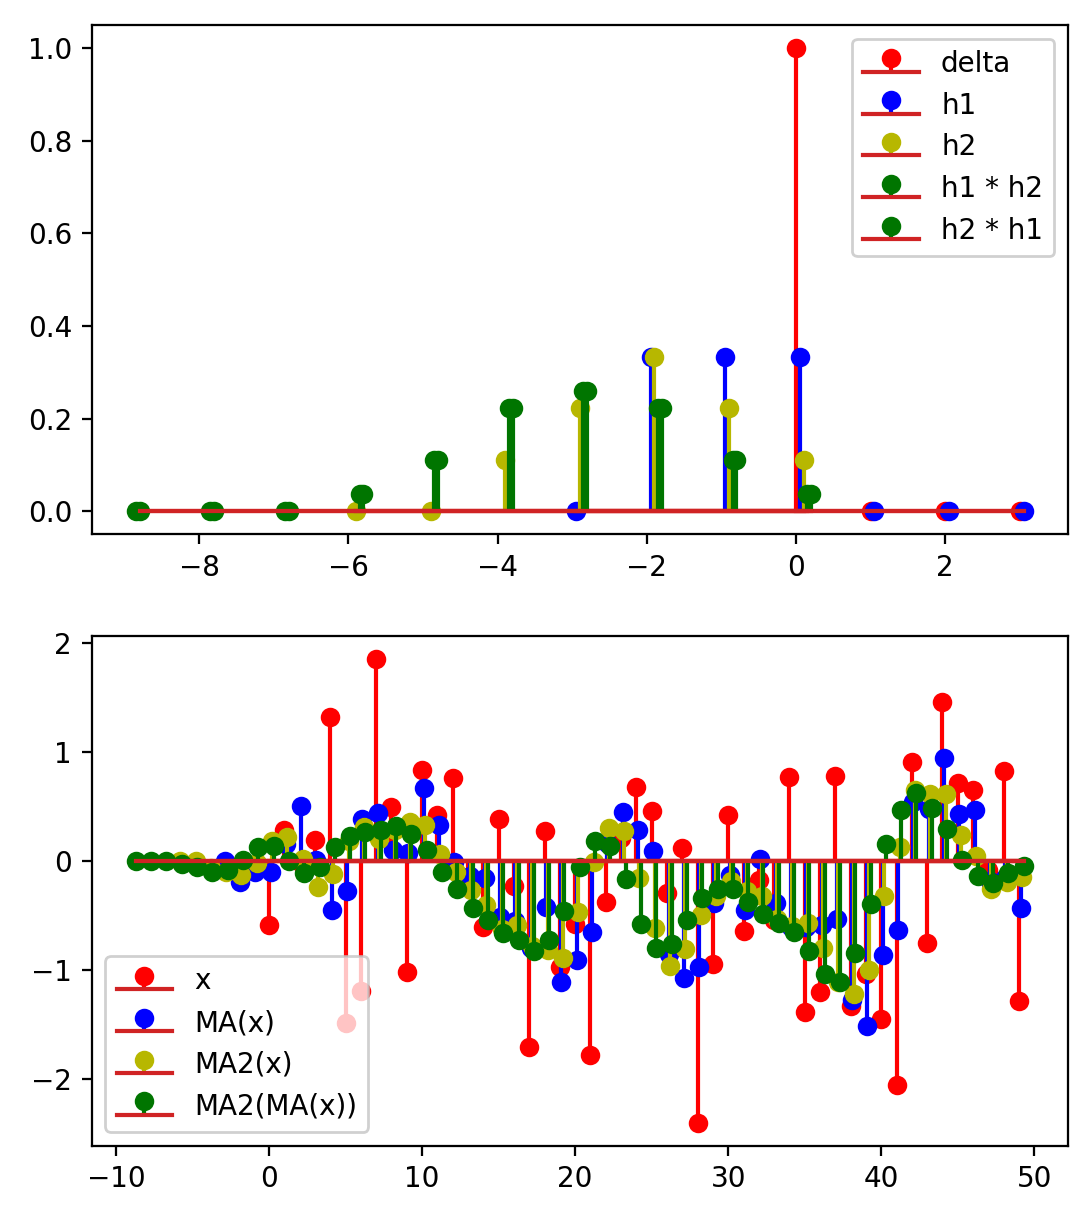
\includegraphics[width=\textwidth]{code/ramp_ma.png}
    \end{minipage}
    \codecaption{dsv/code/ramp_ma.py}{Verkettung von mehreren Moving Averages der L"ange $\ell = 3$.}\label{py:ramp_ma}
\end{listing}
%
In \Cref{py:ramp_ma} untersuchen wir einige der oben genannten Eigenschaften.
Einerseits sehen wir, dass die Impulsantwort von $\texttt{MA}(\texttt{MA2}(\cdot))$ mit der von $\texttt{MA2}(\texttt{MA}(\cdot))$ identisch ist. Wir haben also Kommutativit"at nachgepr"uft.
Wir sehen au"serdem, dass sich die Impulsantwort der Verkettung aus Faltung der einzelnen Impulsantworten ergibt.
Aus dem abgetasteten \q{Rechteck} wird nach nochmaliger Anwendung ein abgetastetes, aber breiteres, \q{Dreieck}, was schlussendlich zu einer abgetasteten, st"uckweise quadratischen, Impulsantwort wird.
Generell kann man das komplette System als eine dreifache Verkettung gleitender Mittel der L"ange $\ell=3$ verstehen.
Au"serdem best"atigt \Cref{py:ramp_ma} bei Vergleich der verschiedenen Ausg"ange, dass wiederholtes Mitteln am Ausgang mit Anzahl der Mittelungen zunehmend \q{glattere} Signale erzeugt.
%
\subsubsection{Eigenschaften von \texorpdfstring{\acrshort{lti}}{LTI}-Systemen}
%
\paragraph{\texorpdfstring{\gls{bibo}}{BIBO}-Stabilit"at}
Wir hatten vorher schon diesen Begriff der Stabili"at eingef"uhrt und formulieren nun eine Bedingung an $h[\cdot]$, die es uns erlaubt auf Stabilit"at zu pr"ufen.
Wir nennen die Eingabe beschr"ankt, falls ein $M_x < \infty$ existiert, sodass
\[
\Abs{x[n]} \leqslant M_x \Text{f"ur alle} n \in \Z
\]
erf"ullt ist.
Dann k"onnen wir mit der Faltungsformel \eqref{eq:lti_sys:conv} berechnen, dass
\[
\Abs{y[n]} 
    = \Abs{\Sum{k\in\Z}{}{x[n] h[n-k]}} 
    \leqslant \Sum{k\in\Z}{}{\Abs{x[n] h[n-k]}} 
    \leqslant M_x \Sum{k\in\Z}{}{\Abs{h[n-k]}} 
\]
gilt.
Damit nun $\Abs{y[n]} < \infty$, muss also gelten, dass
\[
    \Sum{k\in\Z}{}{\Abs{h[n-k]}} < \infty.
\]
Das hei"st, \emph{wenn} $h[\cdot]$ absolut summierbar ist, dann ist das System mit $h[\cdot]$ als Impulsantwort \gls{bibo}-stabil.

Wie ist es um die umgekehrte Schlussfolgerung bestellt?
Impliziert \gls{bibo}-Stabilit"at, dass $h[\cdot]$ absolut summierbar sein muss?
Erinnern wir uns daran, dass man \gls{bibo}-Stabilit"at widerlegen kann, indem man \emph{einen} beschr"ankten Eingang $x[\cdot]$ findet, f"ur welchen der Ausgang $y[\cdot]$ nicht beschr"ankt bleibt.
Nehmen wir an, dass 
\[
\Sum{k\in\Z}{}{\Abs{h[n-k]}} = \infty
\]
und betrachten wir den Eingang
\[
x[n] = \begin{cases}
    \frac{h[-n]^\ast}{\Abs{h[-n]}}, \Text{f"ur} h[n] \neq 0 \\
    0 \Text{sonst.}
\end{cases}
\]
Man sieht, dass $\Abs{x[n]} \leqslant 1$, es ist also beschr"ankt.
Dann berechnen wir einfach den ersten Wert am Ausgang mit \eqref{eq:lti_sys:conv} und der Definition des Einganges $x[\cdot]$, also
\[
y[0] 
    = \Sum{k\in\Z}{}{x[-k] h[k]}
    = \Sum{k\in\Z}{}{
        \frac{\Abs{h[k]}^2}{\Abs{h[k]}}
    }
    = \Sum{k\in\Z}{}{
        \Abs{h[k]}
    }
    = \infty,
\]
wobei das letzte Gleichheitszeichen gilt, weil wir angenommen hatten, dass $h[\cdot]$ nicht absolut summierbar ist.
Man kann also schlussfolgern, dass sich Stabilit"at vollst"andig durch die Impulsantwort $h[\cdot]$ bestimmen l"asst.
Eine tolle Sache!
%
\paragraph{\texorpdfstring{\acrshort{fir}}{FIR} vs. \texorpdfstring{\acrshort{iir}}{IIR}}
%
Gilt f"ur die Impulsantwort $h[\cdot]$, dass
\[
h[n] = 0, \Text{f"ur} n < m, M \leqslant n
\]
f"ur zwei Zahlen $m \leqslant M$, dann bezeichnet man das zugeh"orige System $\mathcal{T}$ als \gls{fir}-System.
Ist obige Bedingung nicht erf"ullt, so nennt man $\mathcal{T}$ ein \gls{iir}-System.
Bei \gls{fir}-Systemen sind f"ur die Berechnung von $y[n]$ nur endlich viele Werte, maximal $M - m$ viele, notwendig.
Das System hat also ein endliches Ged"chtnis der L"ange $M - m$, wobei \gls{iir}-Systeme ein unendlich langes Ged"achtnis haben.
Sobald bei einem \gls{fir}-System $\Abs{h[n]} < \infty$ f"ur alle $n \in \Z$ gilt, ist es auch stabil -- also sind in der Praxis \emph{alle} \gls{fir}-Systeme stabil.

Bei einem \gls{iir}-System ist die Frage nach Stabilit"at nicht so einfach zu beantworten, doch wir werden im Folgenden noch ein Werkzeug kennenlernen, mit welchem dies einfach nachzupr"ufen sein wird.
Au"serdem haben \gls{iir}-Systeme noch das Problem, dass man die Faltungsformel \eqref{eq:lti_sys:conv} nicht nutzen kann, um ein \gls{iir}-System zu \emph{implementieren}.
%
%
\subsubsection{Rekursive \texorpdfstring{\acrshort{iir}}{IIR}-Systeme}
%
%
Um die Notwendigkeit von \eqref{eq:lti_sys:conv} zu umgehen, betrachten wir eine gewisse Klasse von Systemen, deren Ausgang $y[\cdot]$ auch "uber einen alternativen Weg bestimmt werden kann.
Hierzu betrachten wir
\[
y[n] = \frac{1}{n+1}\Sum{k=0}{n}{x[n]},
\]
was ein kumulatives Mittel von $0$ bis $n$ darstellt.
So wie es hier scheint, muss man f"ur die Berechnung von $y[n]$ alle vergangenen Werte von $x[\cdot]$ bereitliegen haben.
Doch mit einer einfachen Umformung findet man, dass
\[
(n+1)y[n] = n y[n-1] + x[n] 
\Leftrightarrow 
y[n] = \frac{n}{n+1} y[n-1] + \frac{1}{n+1} x[n].
\]
Wir k"onnen also alternativ $y[n]$ aus $x[n]$ und $y[n-1]$ berechnen.
Da also $y[n]$ von $y[n-1]$ abh"angt, nennen wir das System \emph{rekursiv}.
Man sieht deutlich, dass diese Umformulierung deutlich macht, dass wir nur $y[n-1]$ im Speicher halten m"ussen und dieses mit einer Art \emph{zeitverz"ogertem Feedback} ausstatten m"ussen.
Hierbei ist nat"urlich die Zeitverz"ogerung essenziell, denn m"ussen wir $y[n]$ in Abh"angigkeit von $y[n]$ berechnen, w"urde uns das vor ein halbwegs unl"osbares Problem stellen.
In \Cref{py:cumulative_sum} sehen wir die beiden unterschiedlichen Implementierungen.
Es ist hier zu beachten, dass \mintinline{python}|y[nn] = np.sum(x[:nn]) / (nn + 1)| immer auf die komplette Vergangenheit von $x[\cdot]$ zugreift und eben \emph{nicht} auf Werte von $y[\cdot]$.

\begin{listing}
    \noindent
    \begin{minipage}{0.49\textwidth}
        \strut\vspace*{-\baselineskip}\newline
        \inputminted[firstline=5,lastline=20]{python3}{code/cumulative_sum.py}
    \end{minipage}%
    \begin{minipage}{0.49\textwidth}
        \strut\vspace*{-\baselineskip}\newline
        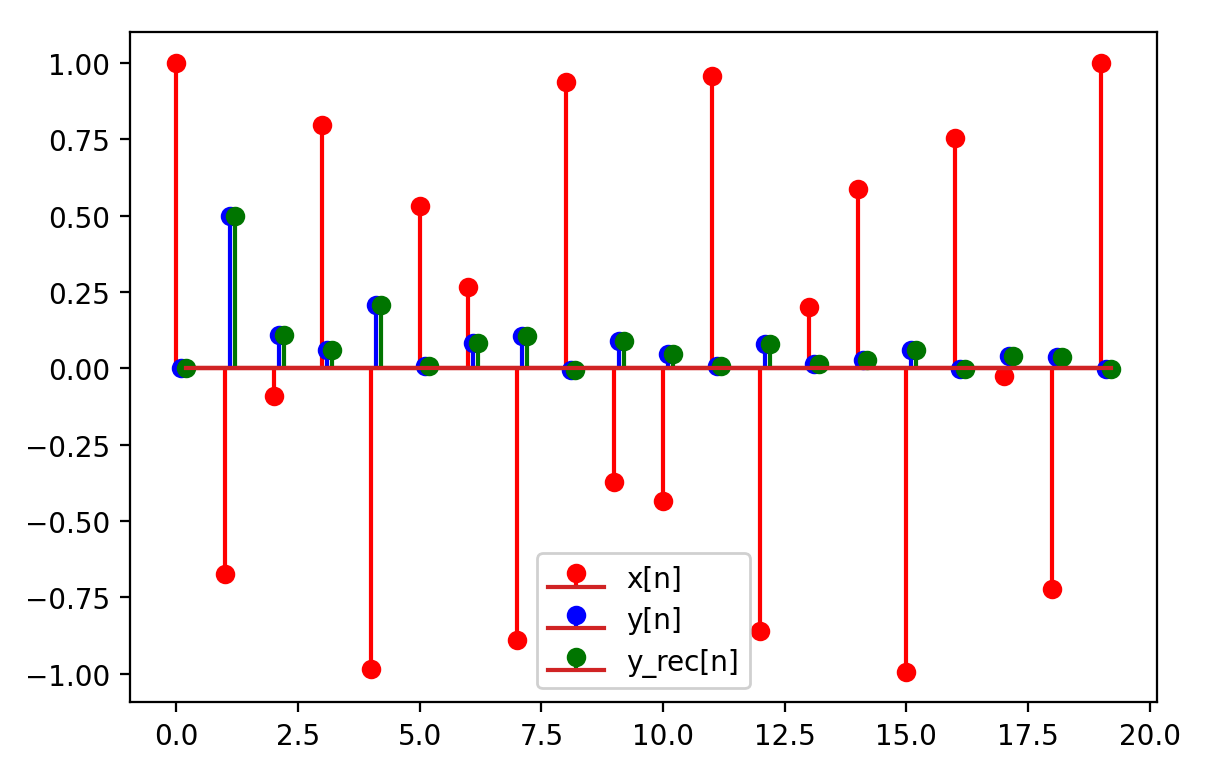
\includegraphics[width=\textwidth]{code/cumulative_sum.png}
    \end{minipage}
    \codecaption{dsv/code/cumulative_sum.py}{Die beiden m"oglichen Implementierungen eines kumulativen Mittelwertes}\label{py:cumulative_sum}
\end{listing}
%
%
F"ur rekursive Systeme entsteht noch das Problem, dass wir beispielsweise f"ur den Beginn der rekursiven Berechnung von $y[n]$ ab einem gewissen $n_0 \in \Z$ den Wert $y[n_0-1]$ kennen m"ussen.
Das hei"st wir ben"otigen einen \emph{Startwert} f"ur die Rekursion.
Dieser beeinflusst auch ma"sgeblich das Verhalten des Systems.

Eine M"oglichkeit, wie man das produktiv ausnutzen kann, ist f"ur die Berechnung der Quadratwurzel einer positiven reellen Zahl $A$.
F"ur die Herleitung definieren wir erst die Funktion $f : \R \rightarrow \R$ via
\[
f(x) = x^2 - A.
\]
Wie man leicht sieht, hat diese Funktion Nullstellen $x_{1,2} = \pm \sqrt{A}$.
Die sogenannte Newton-Iteration~\footnote{\url{https://encyclopediaofmath.org/index.php?title=Newton_method}} berechnet iterativ via
\[
y[n] = y[n-1] - \frac{f(y[n-1])}{f^\prime(y[n-1])}
\]
eine Nullstelle der Funktion $f$.
Setzen wir unsere Funktion ein und definieren $x[\cdot] = A u[\cdot]$, dann erhalten wir
\[
y[n] = \frac 12 \left(
    y[n-1] + \frac{x[n]}{y[n-1]}.
\right)
\]
Nutzen wir einen geeigneten Startwert, beispielsweise $y[-1] = 1$, so erhalten wir eine \emph{sehr schnell} konvergierende Folge von $y[n]$.

\begin{listing}
    \noindent
    \begin{minipage}{0.49\textwidth}
        \strut\vspace*{-\baselineskip}\newline
        \inputminted[firstline=5,lastline=15]{python3}{code/square_root.py}
    \end{minipage}%
    \begin{minipage}{0.49\textwidth}
        \strut\vspace*{-\baselineskip}\newline
        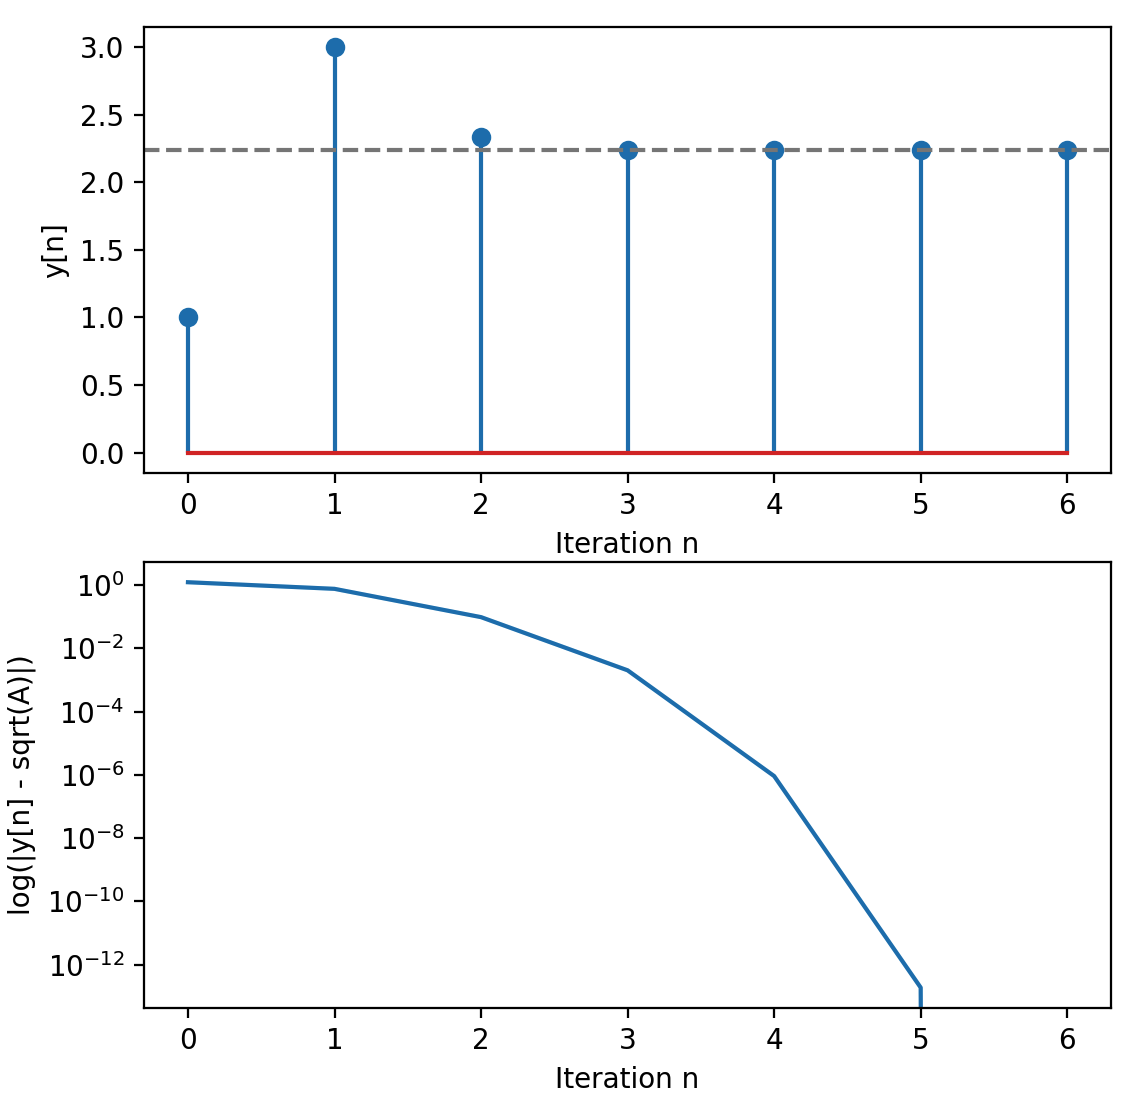
\includegraphics[width=\textwidth]{code/square_root.png}
    \end{minipage}
    \codecaption{dsv/code/square_root.py}{Iteratives Verfahren zur Berechnung von $\sqrt{A}$}\label{py:square_root}
\end{listing}
%
%
Die Folge konvergiert so schnell, dass bereits nach $5$ Iterationen der Fehler an der endlichen Genauigkeit von Gleitkommaarithmetik kratzt.
Es ist auch darauf hinzuweisen, dass das System nur sehr einfache arithmetische Operationen benutzt, um die numerisch nicht ganz triviale Berechnung von $\sqrt{A}$ beliebig genau und sehr schnell zu approximieren.

Abschlie"send ist noch anzumerken, dass man rekursive Systeme auch \q{l"osen} kann, siehe \cite[Kap.~2.4.3]{proakis2013}, indem man aus der rekursiven Vorschrift eine explizite entwickelt. 
Die dort entwickelte Theorie erinnert der L"osung von Differenzialgleichungen nach Funktionen, nur werden stattdessen Differenzengleichungen nach diskreten Folgen gel"ost.
%
%
\subsubsection{Approximation von \texorpdfstring{\acrshort{iir}}{IIR}-Systemen durch \texorpdfstring{\acrshort{fir}}{FIR}-Systeme}
Um die Faltungsformel doch anwenden zu k"onnen, kann man f"ur ein \emph{stabiles} \gls{iir}-System mit Impulsantwort $h[\cdot]$ eine \gls{fir}-Approximation finden.
Ein weiterer Vorteil ergibt sich dann, dass auch dieses resultierende System stabil sein muss.
F"ur $n_{\rm low} < n_{\rm hgh}$ definieren wir
\[
h_{\rm FIR}[n] = \begin{cases}
    h[n], \Text{falls} n_{\rm low} \leqslant n \leqslant n_{\rm hgh}, \\
    0 \Text{sonst.}
\end{cases}
\]
Da aus der Stabilit"at von dem System mit Impulsantwort $h[\cdot]$ folgt, dass
\[
    \lim\limits_{k \rightarrow \infty} 
        \Sum{n = k}{\infty}{
            \left(\Abs{h[n]} + \Abs{h[-n]}\right)
        } = 0,
\]
da sonst
\[
    \Sum{n \in \Z}{\infty}{\Abs{h[n]}}
\]
nicht endlich sein k"onnte.
Das hei"st, dass die Werte der Impulsantwort $h[\cdot]$ gegen $0$ konvergieren m"ussen und deshalb kann man $n_{\rm low} < n_{\rm hgh}$ so w"ahlen, dass der Unterschied zwischen $h[\cdot]$ und $h_{\rm FIR}[\cdot]$ beliebig klein wird.

Je nachdem wie schnell $h[\cdot]$ gegen $0$ konvergiert, ben"otigen wir mehr oder von $0$ verschiedene Eintr"age in $h_{\rm FIR}$, was sich auf den Implementierungsaufwand auswirkt.

Ein Beispiel f"ur einen exponentiellen Mittelwert-Filter findet man in \Cref{py:exp_mean}.
Man sieht, dass f"ur $\alpha=0.5$ der Abschneidefehler deutlicher zutage tritt, da die Faltung mit $h_{\rm FIR}[\cdot]$ in diesem Fall ein deutlich schlechteres Ergebnis liefert als im Falle von $\alpha=0.1$.
Dies liegt eben daran, dass bei $\alpha=0.1$ der \gls{iir}-Filter \emph{effektiv} ein \gls{fir}-Filter wird.
Wir wollen aber darauf hinweisen, dass es eine ganz eigene Theorie f"ur die Approximation von Filtern durch andere Filter gibt, die wir hier nicht einmal anrei"sen wollen.

\begin{listing}
    \noindent
    \begin{minipage}{0.49\textwidth}
        \strut\vspace*{-\baselineskip}\newline
        \inputminted[firstline=5,lastline=33]{python3}{code/exp_mean.py}
    \end{minipage}%
    \begin{minipage}{0.49\textwidth}
        \strut\vspace*{-\baselineskip}\newline
        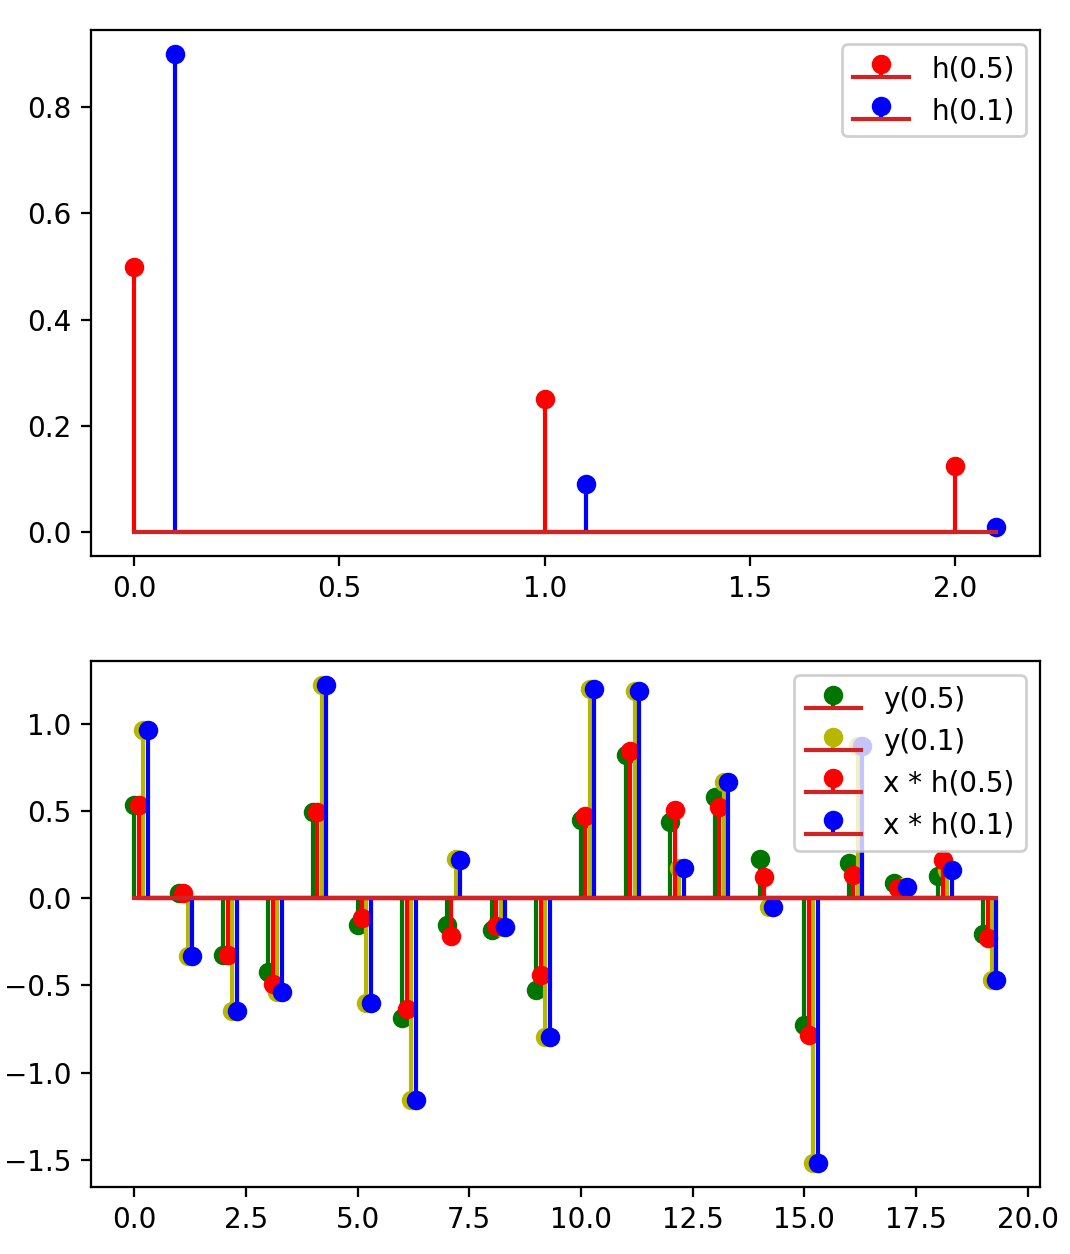
\includegraphics[width=\textwidth]{code/exp_mean.png}
    \end{minipage}
    \codecaption{dsv/code/exp_mean.py}{Approximation eines exponentiellen Mittelwertes, also einem \gls{iir}-System durch ein \gls{fir}-System}\label{py:exp_mean}
\end{listing}
%
\clearpage
\microtypesetup{protrusion=false}
\addcontentsline{toc}{section}{Abk"urzungsverzeichnis}
\printglossary[type=\acronymtype]
\microtypesetup{protrusion=true}
%
%
%
\clearpage
\microtypesetup{protrusion=false}
\addcontentsline{toc}{section}{Literaturverzeichnis}
\printbibliography
\microtypesetup{protrusion=true}
\end{document}
%
%
\section{\texorpdfstring{$z$}{z}-Transformation}\label{ztrafo}
%
Wir wollen nun eines der wichtigsten Werkzeuge f"ur die Analyse von diskreten \gls{lti}-Systemen einf"uhren und untersuchen.
Die $z$-Transformation nimmt f"ur diskrete \gls{lti}-Systeme dieselbe Rolle ein, wie die Laplace-Transformation f"ur zeitstetige \gls{lti}-Systeme.
Wir werden sehen, dass die Faltungs-Formel \eqref{eq:lti_sys:conv} im $z$-Bereich eine einfachere Form annimmt.
Au"serdem erlaubt uns die Transformation eine neue Sicht auf diskrete Systeme zu gewinnen, mit welcher es eventuell einfacher sein sollte gewisse Eigenschaften von Systemen nachzupr"ufen.
Wir werden auch sehen, dass sich manche Signale oder Systeme im $z$-Bereich kompakter aufschreiben lassen.

Die $z$-Transformation $X_\z: \C \rightarrow \C$ eines Signals $x[\cdot] : \N \rightarrow \C$ ist die komplexe Potenzreihe\externallink{{https://mathworld.wolfram.com/LaurentSeries.html}}
\begin{equation}\label{eq:ztrafo:def}
    z \mapsto X_\z(z) = \Sum{n\in\Z}{}{x[n] z^{-n}}.
\end{equation}
Wegen der Summation "uber ganz $\Z$ ist $X_\z(z)$ f"ur jedes $z$ ein Grenzwert, der nicht existieren muss.
Das hei"st, es ist notwendig auch \emph{immer} den Konvergenzbereich, oder Englisch die \gls{roc}, von $X_\z$ anzugeben.

Betrachten wir beispielsweise \[x[\cdot] = \{5,6,\Start{3},4,-\pi\},\] dann ergibt sich \[X_\z(z) = 5 z^2 + 6 z + 3 + 4z^{-1} - \pi z^{-2} \Text{mit \gls{roc}} \C \setminus \{0\}.\] 
Im Fall von $x[\cdot] = \delta[\cdot-k]$, ergibt sich $X_\z(z) = z^{-k}$ mit \gls{roc} $\C \setminus \{0\}$, wobei sich bei $x[\cdot] = \delta[\cdot+k]$, sich $X_\z(z) = z^{k}$ mit \gls{roc} $\C$ ergibt.
Man sieht nun auch, weshalb das System, das ein Signal um einen Abtastwert verz"ogert, oft mit $z^{-1}$ bezeichnet wird, weil dies die $z$-Transformation dessen Impulsantwort ist.
Au"serdem kann man bei endlichen Signalen im $z$-Bereich deren Werte im Zeitbereich einfach ablesen. 
Will man den Wert $x[n]$, also an Sample $n$, ermittelt man diesen, indem man den Koeffizienten vom passenden $z^{-n}$ betrachtet. 

Aber auch f"ur unendlich lange Signale, wie beispielsweise $x[n] = a^n u[n]$, ergibt sich
\[
X_\z(z) 
    = 1 + a z^{-1} + a^2 z^{-2} + \dots
    = \Sum{n = 0}{\infty}{
        a^n z^{-n}
    }
    = \Sum{n = 0}{\infty}{
        \left(a z^{-1}\right)^n
    },
\]
was eine geometrische Reihe "uber $az^{-1}$ darstellt. 
Dann folgt, dass
\[
    X_\z(z) = \frac{1}{1 - a z^{-1}},
\]
wobei diese Potenzreihe nur konvergiert, wenn $z > a$.
Das hei"st, dass die \gls{roc} hier alle $z \in \C$ umfasst mit $\Abs{z} > \Abs{a}$.
Wir sehen, dass sich eigentlich unendlich lange Signale im $z$-Bereich durch Berechnen des Grenzwertes knapper darstellen lassen.
Gleichzeitig k"onnen wir so auch die \gls{roc} bestimmen, indem wir ermitteln, wann der ermittelte Grenzwert existiert.

Wenn wir $z = r\exp(\jmath \phi)$ in die Definition \eqref{eq:ztrafo:def} einsetzen und $\Abs{X_\z(z)}$ betrachten, finden wir
\[
\Abs{X_\z(z)} 
    = \Abs{\Sum{n\in\Z}{}{x[n] z^{-n}}}
    \leqslant \Sum{n\in\Z}{}{\Abs{x[n] z^{-n}}}
    = \Sum{n\in\Z}{}{\Abs{x[n] r^{-n}} \Abs{\exp(- \jmath n \phi)}}
    = \Sum{n\in\Z}{}{\Abs{x[n] r^{-n}}}.
\]
Betrachten wir den letzten Ausdruck genauer indem wir ihn in zwei Summationen aufteilen, also
\[
\Sum{n\in\Z}{}{\Abs{x[n] r^{-n}}} 
    = \Sum{n=-1}{-\infty}{\Abs{x[n] r^{-n}}}
    + \Sum{n=0}{+\infty}{\Abs{x[n] r^{-n}}}
    = \Sum{n=1}{+\infty}{\Abs{x[-n] r^{n}}}
    + \Sum{n=0}{+\infty}{\Abs{\frac{x[n]}{r^{n}}}}.
\]
Das ergibt dann also, dass
\[
    \Abs{X_\z(z)} 
        \leqslant \Sum{n=1}{+\infty}{\Abs{x[-n] r^{n}}}
        + \Sum{n=0}{+\infty}{\Abs{\frac{x[n]}{r^{n}}}}
\]
Damit $X_\z$ existiert, m"ussen beide Grenzwerte existieren.
Der erste Grenzwert existiert, wenn es ein $r_1$ gibt, sodass $r_1^n$ die Werte $x[-n]$ so gewichtet, das sich Konvergenz einstellt. 
Dieses $r_1$ ist ausschlie"slich durch die Werte in der \q{Vergangenheit} von $x[\cdot]$ bestimmt! 
Wenn sich Konvergenz f"ur ein $r_1$ einstellt, dann auch f"ur alle $r < r_1$.
Der Konvergenzbereich ergibt sich also als ein Kreis mit Radius $r_1$.
Der zweite Grenzwert existiert, falls f"ur ein $r_2 > 0$ die Werte $1/r_2^n$ so die \q{Zukunft} von $x[n]$ so wichten, dass die Summe konvergiert.
Das hei"st, falls so ein $r_2$ existiert, dann konvergiert der zweite Summand f"ur alle $r > r_2$.

Die \gls{roc} ist also die Schnittmenge von der Menge $\{\Abs{z} \leqslant r_1\}$ mit der Menge $\{\Abs{z} \geqslant r_2\}$.
Dies ist in \Cref{fig:ztrafo:roc} zusammengefasst. Wir sehen auch, dass im Falle von $r_1 > r_2$ die \gls{roc} die leere Menge ist und deshalb die $z$-Transformation nicht existiert.

\begin{figure}
    \centering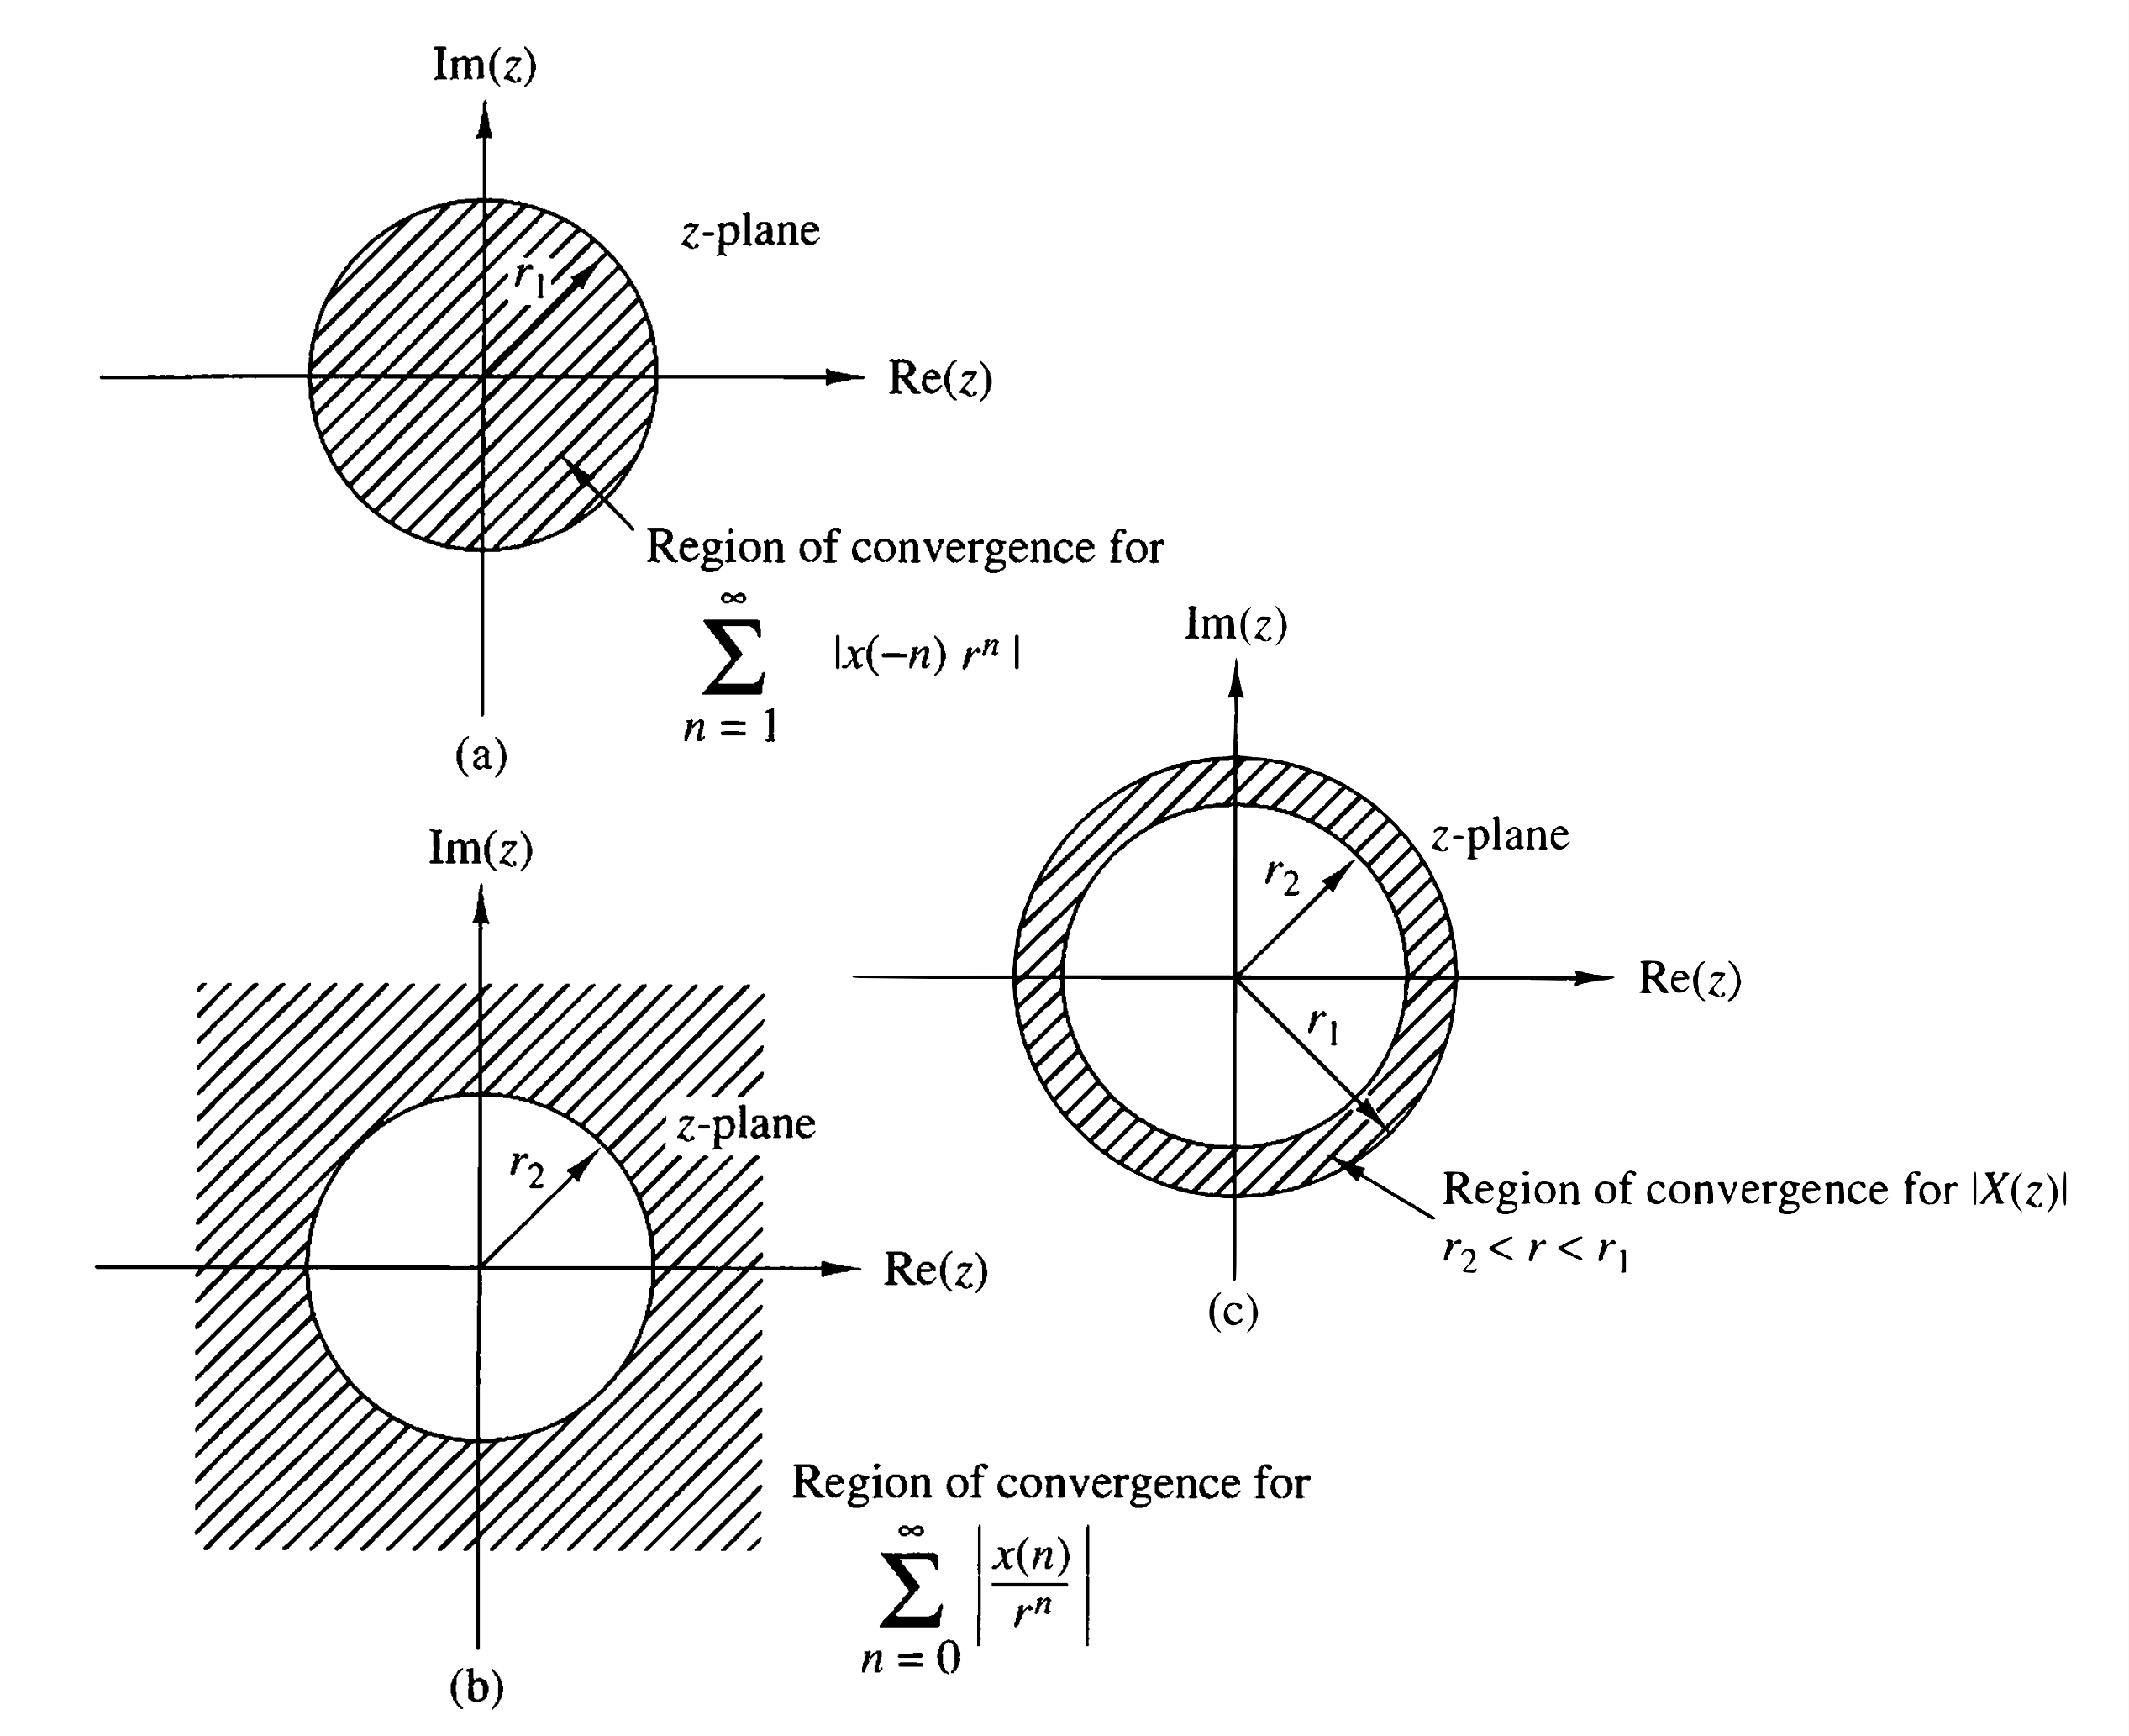
\includegraphics[width=0.8\textwidth]{img/ztrafo/roc.png}
    \caption{Veranschaulichung der Entstehung der \acrshort*{roc} aus den Konvergenzkriterien. Quelle: \cite{proakis2013}}\label{fig:ztrafo:roc}
\end{figure}
%
\subsubsection{Eigenschaften}\label{sec:ztrafo:properties}
%
Wir wollen nun einige Eigenschaften der $z$-Transformation auflisten, die wir immer wieder verwenden werden. 
Besonderes Augenmerk legen wir hierbei auf die Behandlung der \gls{roc}.
%
\paragraph{Linearit"at}
Gegeben zwei diskrete Signale $x_{1,2}[\cdot]$ und komplexe Zahlen $a_{1,2} \in \C$, dann gilt f"ur $x[\cdot] = a_1 x_1[\cdot] + a_2 x_2[\cdot]$, dass
\[
X_\z(z) = a_1 X_{\z,1}(z) + a_2 X_{\z, 2}(z),
\]
wobei die \gls{roc} von $X_{\z}$ der Schnittmenge der \glspl{roc} von $X_{\z,1}$ und $X_{\z,2}$ entspricht.
%
\paragraph{Zeitversatz}
Ist $X_\z$ die $z$-Transformation von $x[\cdot]$, so ist $z^{-k}X(z)$ die $z$-Transformation von $x[\cdot - k]$.
Hierbei ist die \gls{roc} von $X_{\z}$, falls $k\leqslant 0$.
Im Falle $k>0$ m"ussen wir aus der \gls{roc} von $X_{\z}$ den Wert $z=0$ entfernen.
Intuitiv sollte man diese Eigenschaft leicht verifizieren k"onnen, da man durch das Verschieben nur die Potenz des $z$ "andert und man diese "Anderung einfach ausklammern kann.

Um beispielsweise die $z$-Transformation von
\[
x[n] = \begin{cases}
    1, \Text{f"ur} 0 \leqslant n < N \\
    0 \Text{sonst}, 
\end{cases}
\]
zu bestimmen, k"onnten wir einerseits die Definition bem"uhen, oder die beiden schon bekannten Eigenschaften ausnutzen, um zu folgern, dass
\[
X_\z(z) = \begin{cases}
    N \Text{f"ur} z = 1,\\
    \frac{1 - z^{-N}}{1 - z^{-1}}
\end{cases}
\]
gilt.
Dazu nutzen wir, dass $x[n] = u[n] - u[n-N]$ gilt.
Da au"serdem $x[\cdot]$ nur endlich viele Werte verschieden von $0$ hat, ist die \gls{roc} von $X_\z$ die ganze $z$-Ebene, au"ser $z=0$.
%
\paragraph{Skalierung im \texorpdfstring{$z$}{z}-Bereich}
Ist $X_\z$ die $z$-Transformation von $x[\cdot]$ mit \gls{roc} $r_1 < \Abs{z} < r_2$, dann ist $a^n x[n]$ die inverse $z$-Transformation von $X(a^{-1} z)$ mit \gls{roc} $\Abs{a}r_1 < \Abs{z} < \Abs{a}r_2$.
Die Intuition hierbei ist, dass die Multiplikation mit der Folge $a^{n}$ mit $a=r\exp(\jmath \omega)$ eine Skalierung um $r$ und eine Rotation um $\omega$ im $z$-Bereich bewirkt.
Das hei"st gewisse \q{geometrische} Eigenschaften von $X_{\z}$ transformieren sich analog mit.
%
\paragraph{Zeitumkehrung}
Ist $X_\z$ die $z$-Transformation von $x[\cdot]$ mit \gls{roc} $r_1 < \Abs{z} < r_2$, dann ist $X_{\z}\left(z^{-1}\right)$ die $z$-Transformation von $x[-\cdot]$ mit \gls{roc} $1/r_1 < \Abs{z} < 1/r_2$.
Mit anderen Worten entspricht Umkehrung im Zeitbereich Reflexion am Einheitskreis im $z$-Bereich.
%
\paragraph{Faltung im Zeitbereich}
%
Kommen wir nun zu einer der wichtigsten Eigenschaften und einem der Gr"unde, weshalb die $z$-Transformation als Analogie zur Laplace-Transformation verstanden wird.
Gegeben zwei diskrete Signale $x_{1,2}[\cdot]$ und $x[\cdot] = x_1 \ast x_2$, dann gilt 
\begin{equation}\label{eq:ztrafo:conv}
    X_{\z}(z) = X_{\z,1}(z) \cdot X_{\z,2}(z),
\end{equation}
wobei die \gls{roc} mindestens die Schnittmenge der \glspl{roc} von $X_{\z,1}(z)$ und $X_{\z,2}(z)$ ist.
Der Grund f"ur das \q{mindestens} ist die Tatsache, dass f"ur gewisse $z$ die Divergenz von $X_{\z,1}$ durch rasches Tendieren von $X_{\z,2}$ gegen $0$ kompensiert werden kann.

Wegen ihrer Bedeutung, wollen wir uns kurz "uberlegen, warum die obige Eigenschaft gilt.
Wir nutzen im Grunde nur die Definition \eqref{eq:ztrafo:def} und die Definition der Faltung, um zu sehen, dass
\[
X_\z(z) 
    = \Sum{n \in \Z}{}{x[n] z^{-n}} 
    = \Sum{n \in \Z}{}{
        \Sum{k \in \Z}{}{x_1[k] x_2[n - k]} z^{-n}
      } 
    = \Sum{k \in \Z}{}{
        x_1[k] \Sum{n \in \Z}{}{x_2[n - k]} z^{-n}
    }.
\]
Jetzt nutzen wir die Eigenschaft, die sich aus dem Zeitversatz gibt zusammen mit \eqref{eq:ztrafo:def}, und erhalten schlussendlich
\[
    X_\z(z) 
    = \Sum{k \in \Z}{}{
        x_1[k] \Sum{n \in \Z}{}{x_2[n - k]} z^{-n}
    } 
    = \Sum{k \in \Z}{}{
        x_1[k] X_{\z, 2}(z) z^{-k}
    }
    = X_{\z, 2}(z) \Sum{k \in \Z}{}{
        x_1[k] z^{-k}
    }
    = X_{\z,1}(z) X_{\z, 2}(z).
\]
Wir k"onnen also zusammenfassend folgende Herangehensweise bei der Berechnung der Faltung angeben:
\begin{enumerate}
    \item Transformation von $x_{1,2}[\cdot]$ zu $X_{\z,1,2}$
    \item Punkweise Multiplikation von $X_{\z}(z) = X_{\z,1}(z) X_{\z,2}(z)$
    \item R"ucktransformation von $X_{\z}(z)$ zu $x[\cdot] = x_1 \ast x_2$
\end{enumerate}
%
\paragraph{Inverse \texorpdfstring{$z$}{z}-Transformation}
Obige Berechnung der Faltung verlangt im letzten Schritt die Invertierung der $z$-Transformation von $X_{\z}$ zu $x[\cdot]$.
Im allgemeinen Fall ist man darauf angewiesen den Cauchyschen Integralsatz~\externallink{{https://de.wikipedia.org/wiki/Cauchyscher_Integralsatz}} zu bem"uhen.
Am Ende erlaubt dieser die Herleitung von
\begin{equation}\label{eq:ztrafo:inv}
    x[n] = \frac{1}{\jmath 2 \pi} \ointctrclockwise\limits_{C \subset \mathrm{ROC}} X_{\z}(z) z^{n-1} \mathrm{d}z
\end{equation}
als M"oglichkeit der Bestimmung von $x[n]$ aus $X_{\z}$.
Oft sind diese Integrale jedoch nicht leicht zu Berechnen und man sollte sich auf geeignete Tabellen (siehe~\cite[Tabelle~3.2,~Tabelle~3.3]{proakis2013}) und die restlichen obigen Eigenschaften beziehen, wenn man $z$-Transformationspaare bestimmen m"ochte.
%
%
\subsubsection{Anwendung bei diskreten \texorpdfstring{\acrshort*{lti}}{LTI}-Systemen}
%
Wir kombinieren nun \eqref{eq:lti_sys:conv} mit \eqref{eq:ztrafo:conv}, um eine alternative Beschreibung von \gls{lti}-Systemen zu erhalten.
Wir wissen aus \eqref{eq:lti_sys:conv}, dass sich das Eingabe-Ausgabe-Verhalten von einem \gls{lti}-System $\mathcal{T}$ durch
\[
y[\cdot] = h \ast x
\]
ausdr"ucken l"asst, wobei $h[\cdot] = y[\cdot]$ f"ur $x[\cdot]=\delta$.
Im $z$-Bereich transformiert sich dies wegen \eqref{eq:ztrafo:conv} zu
\begin{equation}\label{eq:ztrafo:transfer_function}
    Y_\z(z) = H_\z(z) X_\z(z).
\end{equation}
Man nennt dann $H_{\z}$ als $z$-Transformation der Impulsantwort die \emph{Transferfunktion} des Systems $\mathcal{T}$.
Wir haben so eine alternative Sichtweise auf \gls{lti}-Systeme gewonnen, weil man eben durch die $z$-Transformation die Impulsantwort $h[\cdot]$ mit der Transferfunktion $H$ \emph{identifiziert}.
Das hei"st, dass beide Beschreibungen "aquivalent sind.
Wir werden uns wie in \Cref{sec:lti_sys:properties} "uberlegen, wie man gewissen Eigenschaften von \gls{lti}-Systemen an $H$ \q{ablesen} kann.

Aus diesem multiplikativen Zusammenhang kann man bei Kenntnis von zwei Gr"o"sen in der Regel die fehlende Dritte bestimmen.
Kennt man beispielsweise $H_\z$ und $X_\z$, dann kann man sehr einfach $Y_\z$ und damit auch $y[\cdot]$ bestimmen.
In bestimmten Anwendungen der Messtechnik ist man eher daran interessiert durch geschickte Messungen $h[\cdot]$ zu bestimmen.
Dies kann unter anderem interessant sein, wenn in $h[\cdot]$ gewisse Parameter eines Systems \q{versteckt} sind, die einen aber interessieren.
Dann ist es oft geschickt das System durch $x[\cdot]$ anzuregen, $y[\cdot]$ zu beobachten und dann die Transferfunktion durch
\[
H_\z(z) = \frac{Y_\z(z)}{X_\z(z)}
\]
zu bestimmen.
Man muss sich im Klaren hierbei sein, dass es hierzu notwendig ist das Signal $x[\cdot]$ so zu w"ahlen, dass obige Division ein hinreichend genaues Bild von $h[\cdot]$ erlaubt.
%
%
\paragraph{Rekursive Systeme}
Ist allgemein die Vorschrift von einem System gegeben durch
\[
y[n] = -\Sum{k=1}{N}{a_k y[n-k]} + \Sum{k=0}{M}{b_k x[n - k]},
\]
dann ergibt sich durch die Linearit"at, Zeitversatz und geschicktes Umstellen, dass
\[
    H(z) = \frac{\Sum{k=0}{M}{b_k z^{-k}}}{1 + \Sum{k=1}{N}{a_k z^{-k}}}.
\]
Das hei"st, dass Systeme, die durch lineare Differenzengleichungen charakterisiert sind, besitzen eine Transferfunktion, die die Struktur einer rationalen Funktion
\[
H_\z(z) = \frac{B(z)}{A(z)}
\]
hat, wenn wir fordern, dass $A$ und $B$ Polynome in $z$ sind.
Allgemein schreiben wir
\[
H(z) = 
    \frac{
        b_0 + b_1 z^{-1} + \dots + b_M z^{-M}
    }{
        a_0 + a_1 z^{-1} + \dots + a_N z^{-N}
    }
    = \frac{
        \Sum{k = 1}{M}{b_k z^{-k}}
    }{
        \Sum{k = 1}{N}{a_k z^{-k}}
    }
    = G z^{N - M} \frac{
        (z - z_1) \dots (z - z_M)
    }{
        (z - p_1) \dots (z - p_N)
    }.
\]
Dann nennen wir die $z_1, \dots, z_M$ die \q{Nullstellen}, oder \emph{zeros}, des Systems $\mathcal{T}$ und die Menge $p_1 ,\dots, p_N$ die \emph{Pole}, oder \emph{Polstellen}, von $\mathcal{T}$.
Tritt ein $p_i$ oder $z_i$ mehrfach auf, so sprechen wir von einer mehrfachen Polstelle, bzw.\,Nullstelle.
Die Anzahl an gleichen Null-/Polstellen nennt man ihre Vielfachheit.

Es gibt nun zwei Spezialf"alle, die wir betrachten k"onnen. 
Erstens, es gilt $a_1 = \dots = a_N = 0$. 
In diesem Fall gilt 
\[
H(z) = z^{-M} \Sum{k = 1}{M}{b_k z^{M-k}}
\]
und $H$ besitzt als Polynom vom Grad $M$ dann $M$ Nullstellen~\externallink{{https://de.wikipedia.org/wiki/Fundamentalsatz_der_Algebra}} und eine $M$-fache Polstelle bei $z=0$.
Tritt eine Polstelle bei $z=0$ auf, so nennen wir diese \emph{trivial}, da sie keinen Einfluss auf das System hat.
Schlie"slich korrespondiert $z^{-M}$ nur zu einer Verschiebung im Zeitbereicht, was bei \gls{lti}-Systemen per definitionem nur eine globale Verschiebung der ganzen Systems bedeutet.
Da keine nicht-trivialen Polstellen auftreten, hat das System eine \emph{endliche} Impulsantwort.
Das k"onnen wir daran sehen, dass wir die Werte von $h[\cdot]$ direkt an den Koeffizienten von $H$ ablesbar sind.

Zweitens, kann es vorkommen, dass $b_1 = \dots = b_N = 0$, was wiederum $H$ zu einer rationalen Funktion macht, die keine Nullstellen und dementsprechend ausschlie"slich Polstellen besitzt.
Um zu bestimmen, welche Implikation dies hat, betrachten wir ein einfaches System mit einem reellen Pol bei $a \in \R$, also
\[
H(z) = \frac{1}{1 - a z^{-1}}, ROC: \Abs{z} > \Abs{a}.
\]
Wie wir weiter oben schon gesehen haben, ist die zugeh"orige Impulsantwort $h[\cdot]$ gegeben durch
\[
h[n] = a^n u[n].
\]
%
\begin{figure}
    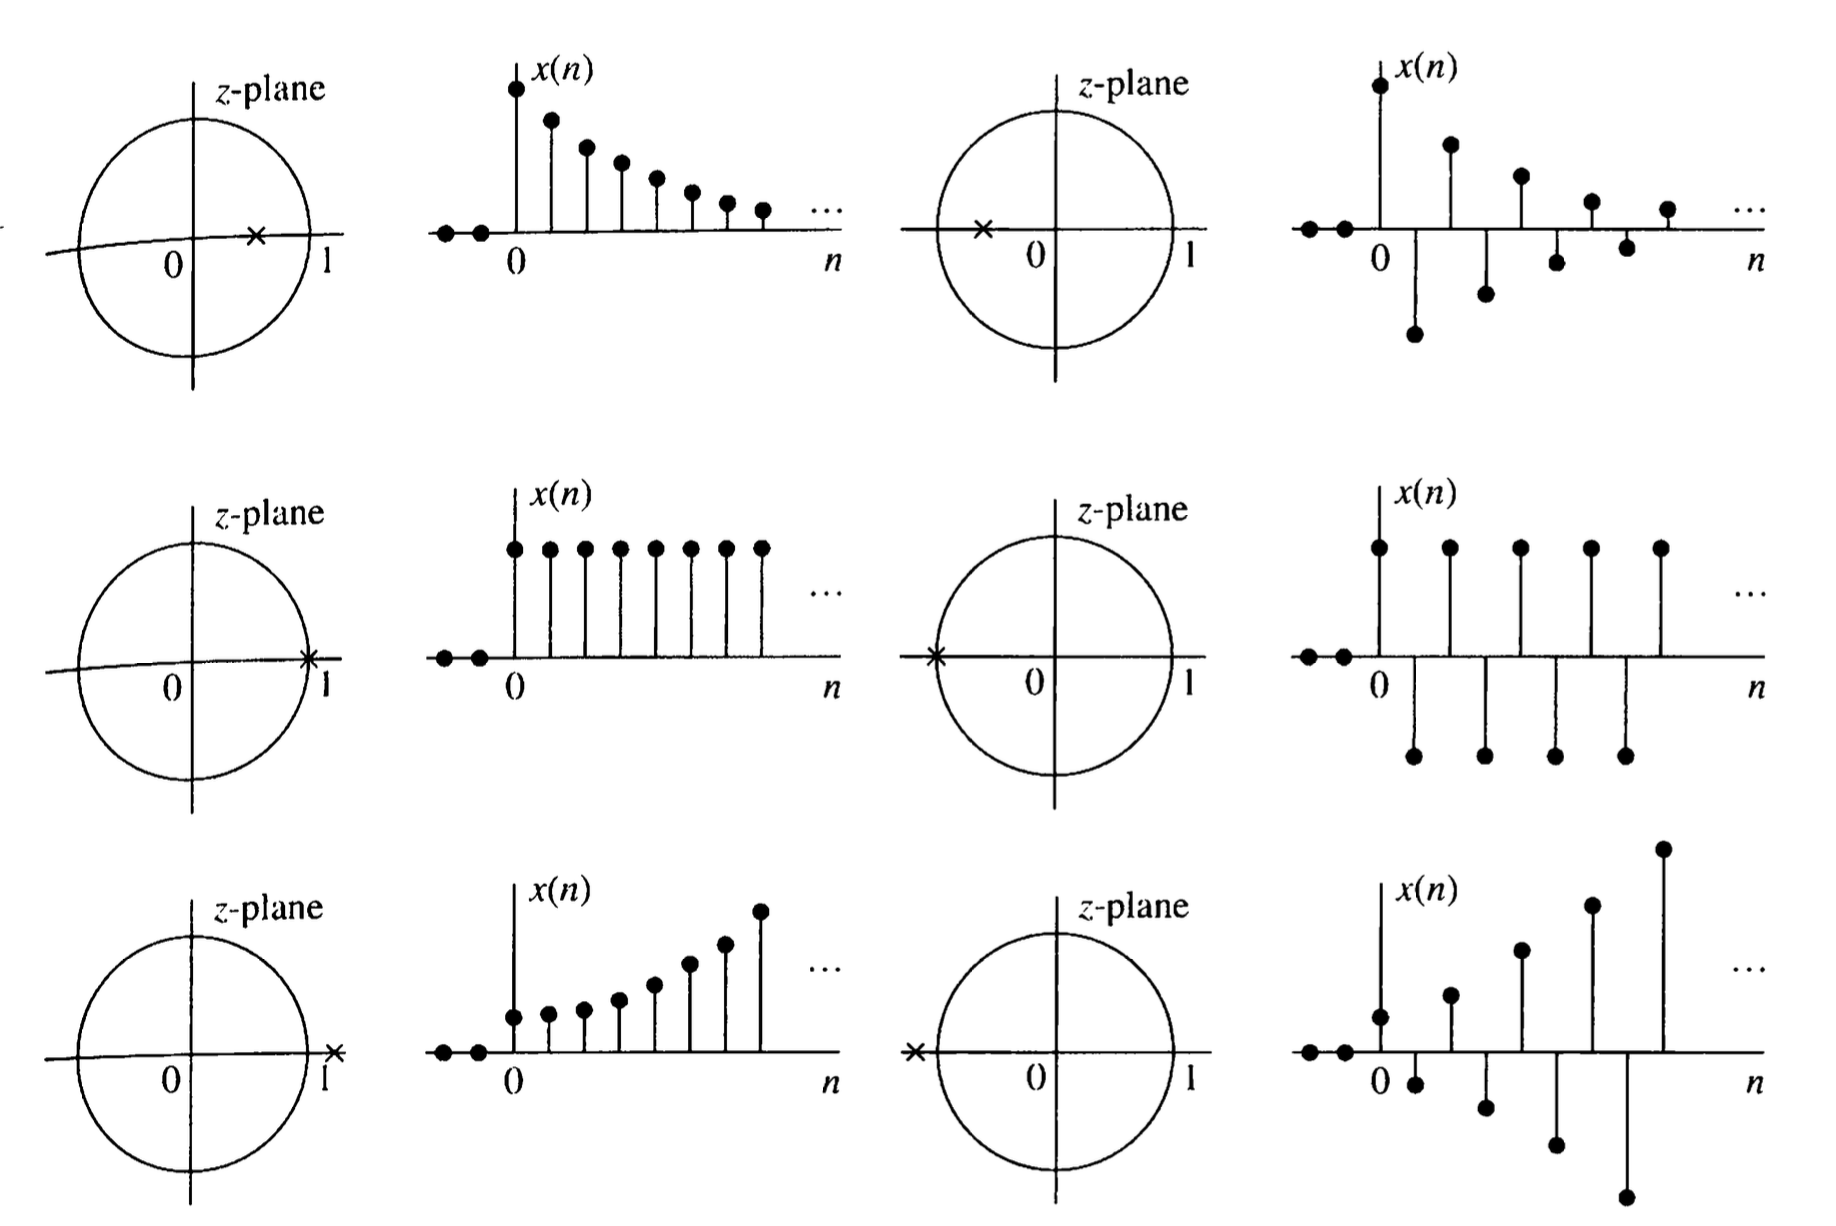
\includegraphics[width=0.9\textwidth]{img/ztrafo/singlepole.png}
    \caption{Impulsantwort $h[n] = a^n u[n]$ f"ur verschiedene Werte von $a$, Quelle: \cite{proakis2013}}\label{fig:ztrafo:singlepole}
\end{figure}

Das Verhalten von diesem System ist in \cref{fig:ztrafo:singlepole} dargestellt.
Man sieht, dass der Einheitskreis in der komplexen Ebene eine entscheidende Rolle spielt.
Liegt $a$ innerhalb des Einheitskreises, so ergibt sich eine exponentiell abfallende Impulsantwort.
Falls $a < 0$, stellt sich auch eine Oszillation ein.
F"ur $\Abs{a} = 1$ entspricht der Betrag der Impulsantwort der Heavyside-Funktion $u[\cdot]$.
Man sieht, dass im Fall von $\Abs{a} < 1$ die Impulsantwort absolut summierbar ist, also
\[
\Sum{n \in \Z}{}{\Abs{h[n]}} < \infty,
\]
was impliziert, dass das System stabil ist.
Entsprechend, ist das System instabil, falls $\Abs{a} > 1$.
Man sieht also, dass die Position der Pole im $z$-Bereich direkt interpretierbar ist.
Betrachtet man nochmals die \gls{roc} $\Abs{z} > \Abs{a}$, zusammen mit der Information, dass sich Stabilit"at einstellt, falls $\Abs{a}<1$.
Geometrisch bedeutet dies, dass das System stabil ist, falls der Einheitskreis in der \gls{roc} enthalten ist.

Diese Resultate lassen sich auf mehrere Polstellen verallgemeinern, da $H$ nur mehr Pole enth"alt und die \gls{roc} dann sich nach dem Betrag der \q{gr"o"sten} Polstelle richtet.
Das hei"st ultimativ, dass sich f"ur ein System $H$ Stabilit"at einstellt, falls \emph{alle} Polstellen sich im Einheitskreis befinden, \emph{oder} "aquivalent, dass sich der Einheitskreis in der \gls{roc} befinden muss.
Sp"ater werden wir noch eine Bedingung f"ur Stabilit"at in Bezug auf die Fourier-Transformation finden.

%
%
\section{Fourier-Transformation}\label{fourier}
%
Wir wollen unsere Werkzeuge zur Analyse von Signalen und Systemen nun um das wahrscheinlich wichtigste erweitern.
Hierbei zerlegen wir Signale, beziehungsweise Systemantworten/Impulsantworten, in ihre \q{harmonischen} Anteile -- wir transformieren in den \emph{Frequenzbereich}.
Man diese Art der \emph{Analyse} auch oft \emph{Fourier-Analyse}.
Da wir verschiedene Arten von Signalen bereits kennengelernt haben, muss diese Zerlegung auch auf verschiedene Weisen durchgef"uhrt werden.
F"ur diskrete Signale, ergibt es beispielsweise wenig Sinn, eine Integraltransformation zu definieren, Aperiodische Signale wiederum k"onnen nicht in einer Fourier-Reihe entwickelt werden, da die inh"arent der Periodizit"at widerspricht.
Das hei"st, dass f"ur jede \q{Art} von Signal und dessen Eigenschaften, die passende Transformation existiert.
Weiterhin "andert sich auch immer die \emph{Interpretation} dieser Zerlegung in harmonische Komponenten.

Dar"uber hinaus werden wir auch den umgekehrten Weg gehen.
Es ist auch m"oglich, Signale aus dem Frequenzbereich in den jeweils richtigen Definitionsbereicht zu transformieren. 
In diesem Fall spricht von von \emph{Fouriersynthese}, da wir ein Signal aus dessen Information "uber harmonische Anteile erzeugen/synthetisieren.
Wir liefern nun also die Definitionen und Zusammenh"ange der Fourier-Transformation, die wir in \Cref{sec:sampling} ohne Erl"auterungen ausgenutzt haben.

\subsection{Fourier-Transformation kontinuierlicher Signale}\label{sec:fourier:cont}

\subsubsection{Fourier-Transformation kontinuierlicher periodischer Signale}\label{sec:fourier:cont:period}

Wir haben bereits in \Cref{sec:cont_complex_harm} mit \eqref{eq:cont_fourier_series} gesehen, dass man durch Linearkombination der komplexen Sinus-Funktionen
\[
\{\exp(\jmath 2 \pi k F_0 t), \fuer k \in \Z\}
\]
eine $1/F_0=T_0$-periodische Funktion $x: \R \rightarrow \C$ durch
\[
x(t) = \Sum{k \in \Z}{}{c_k \exp(\jmath 2 \pi k F_0 t)}
\]
erh"alt.
Dies ist demnach ein Fall von \emph{Fourier-Synthese}, da wir aus den Gewichten $c_k$ in der Linearkombination eine Funktion $x$ erhalten.
Wir wollen nun den umgekehrten Weg gehen, auf welchem wir f"ur eine gegebene Funktion $x$ die Koeffizienten $c_k$ bestimmen k"onnen.
Wir starten dazu mit 
\begin{equation}\label{eq:fourier:fourier_series}
    x(t) = \Sum{k \in \Z}{}{
        c_k \exp(\jmath 2 \pi k F_0 t)
    }
\end{equation}
und multiplizieren beide Seiten mit $\exp(-\jmath 2 \pi \ell F_0 t)$ und integrieren "uber eine Periode $[0,T_0]$.
Dann erhalten wir
\[
\Int{0}{T_0}{
    x(t) \exp(-\jmath 2 \pi \ell F_0 t)
}{t} 
= \Int{0}{T_0}{
    \left(
        \Sum{k \in \Z}{}{
            c_k \exp(\jmath 2 \pi k F_0 t)
        }
    \right)
    \exp(-\jmath 2 \pi \ell F_0 t)
}{t} 
\]
und nach Vertauschung von Summation und Integration, dass
\[
\Sum{k \in \Z}{}{
    c_k 
    \Int{0}{T_0}{\exp(\jmath 2 \pi (k - \ell) F_0 t)}{t}
}
= \Sum{k \in \Z}{}{
    c_k \left[
        \frac{
            \exp(-\jmath 2 \pi (k - \ell) F_0 t)
        }{
            \jmath 2 \pi F_0(k - \ell)
        }
    \right]_{0}^{T_0}
}.
\]
Da die Funktion $\exp(-\jmath 2 \pi (k - \ell) F_0 t)$ im Fall $k \neq  \ell$ Periode $T_0$ besitzt, sind alle Summanden in der rechten Summation identisch $0$, au"ser wenn $k = \ell$.
Dann ergibt sich f"ur $\exp(\jmath 2 \pi (k - \ell) F_0 t) = 1$, also
\[
\Int{0}{T_0}{\exp(\jmath 2 \pi (k - \ell) F_0 t)}{t} 
    = \Int{0}{T_0}{1}{t} 
    = T_0.
\]
Final erhalten wir f"ur die Berechnung der Fourier-Koeffizienten $c : \N \rightarrow \C$ als Berechnungsvorschrift
\[
    c[\ell] = \frac{1}{T_0}\Int{0}{T_0}{
        x(t) \exp(-\jmath 2 \pi \ell F_0 t)
    }{t}.
\]
Wir haben in diesem Fall also \emph{Fourier-Analyse} betrieben.
Au"serdem haben wir absichtlich die Schreibweise von $c_\ell$ auf $c[\cdot]$ angepasst, um zu verdeutlichen, dass man nun die $c[\cdot]$ als \emph{komplexes diskretes Signal} auffassen k"onnen.
Dieses diskrete Signal k"onnen wir nun durch die Fourier-Reihe mit dem Signal $x : \R \rightarrow \C$ \emph{identifizieren}.
Sowohl $x$ als auch $c[\cdot]$ sind also Darstellungen desselben Sachverhaltes -- im \q{Zeitbereich} und im zugeh"origen \q{Frequenzbereich}.
Wir sehen auch, dass sich f"ur kontinuierliche und periodische Signale ein \emph{diskreter} Frequenzbereich ergibt.

Obige Herleitung verschleiert aber einen viel tiefer liegenden Zusammenhang.
Definieren wir wie in \Cref{sec:cont_complex_harm} die Funktionen $x_k : \R \rightarrow \C$ als
\[
x_k(t) = \exp(\jmath 2 \pi k F_0 t),
\]
dann k"onnen wir obige Rechnung auch so auffassen.
Wir betrachten Multiplikation von $x$ mit $x_\ell^\ast$ und anschlie"sende Integration als Skalarprodukt $\ScPr{x}{x_\ell}$. 
Au"serdem haben wir aus der Fourier-Reihe gegeben, dass
\[
x = \Sum{k \in \Z}{}{c_k x_k}
\]
Wir haben also in dieser Denkweise lediglich auf beiden Seiten der Fourierreihe in \eqref{eq:fourier:fourier_series} das Skalarprodukt mit $x_\ell$ gebildet.
Also
\[
\ScPr{x}{x_\ell} = \ScPr{\Sum{k \in \Z}{}{c_k x_k}}{x_\ell}.
\]
Das Skalarprodukt ist linear, also k"onnen wir auch
\[
\ScPr{x}{x_\ell} = \Sum{k \in \Z}{}{c_k \ScPr{x_k}{x_\ell}}
\]
schreiben.
Wir m"ussen also nur $\ScPr{x_k}{x_\ell}$ bestimmen. 
Dies haben wir aber oben schon berechnet, denn das waren die Ausdr"ucke
\[
\ScPr{x_k}{x_\ell}
    = \Int{0}{T_0}{x_k(t) x_\ell(t)^\ast}{t}
    = \Int{0}{T_0}{\exp(\jmath 2 \pi k F_0 t) \exp(-\jmath 2 \pi \ell F_0 t)}{t}
    = \Int{0}{T_0}{\exp(\jmath 2 \pi (k - \ell) F_0 t)}{t}
\]
Von oben wissen wir, dass
\[
\ScPr{x_k}{x_\ell} 
    = \left[
        \frac{
            \exp(-\jmath 2 \pi (k - \ell) F_0 t)
        }{
            \jmath 2 \pi F_0(k - \ell)
        }
    \right]_{0}^{T_0}
    = \begin{cases}
        T_0 \fuer k = \ell \\
        0, \Text{sonst.}
    \end{cases}
\]
Die $x_k$ stehen also paarweise \emph{senkrecht/orthogonal} zu einander und es gilt $\ScPr{x}{x_\ell} = T_0$.
Sie bilden ein sogenannten \emph{Orthogonalsystem}.
H"atten wir $\hat{x}_k = x_k / \sqrt{T_0}$ definiert, w"urde sogar gelten $\ScPr{\hat{x}_k}{\hat{x}_k} = 1$ und die $\hat{x}_k$ bilden eine \emph{Orthonormalsystem}.

Wenn wir nun noch einmal obige Gleichung f"ur $\ScPr{x}{x_\ell}$ betrachten, finden wir
\[
\ScPr{x}{x_\ell} 
    = \Sum{k \in \Z}{}{c_k \ScPr{x_k}{x_\ell}}
    = T_0 c_\ell,
\]
weil alle Summanden durch die Orthogonalit"at verschwinden und nur im Falle von $k = \ell$ eben $T_0$ "ubrig bleibt.
Der Fourier-Koeffzient $c_\ell$ ergibt sich also als Skalarprodukt von $x$ mit dem zugeh"origen $x_\ell$.
Es ist wichtig zu sehen, dass wir nur f"ur die Berechnung von $\ScPr{x_k}{x_\ell}$ die spezielle Form der $x_k$ eingesetzt haben und sonst nur allgemein mit den Eigenschaften von Skalarprodukten gearbeitet haben.
Das hei"st, dass man ganz allgemein Signale \q{transformieren} beziehungsweise \emph{analysieren} kann, indem man sie als Summe von paarweise orthogonalen Signalen ausdr"uckt.
Die Fourier-Reihe ist nur ein Spezialfall von diesem allgemeinen Konzept!

\begin{listing}[ht]
    \noindent
    \begin{minipage}{0.51\textwidth}
        \strut\vspace*{-\baselineskip}\newline
        \inputminted[firstline=10, lastline=44]{python3}{code/fourier_series.py}
    \end{minipage}%
    \begin{minipage}{0.48\textwidth}
        \strut\vspace*{-\baselineskip}\newline
        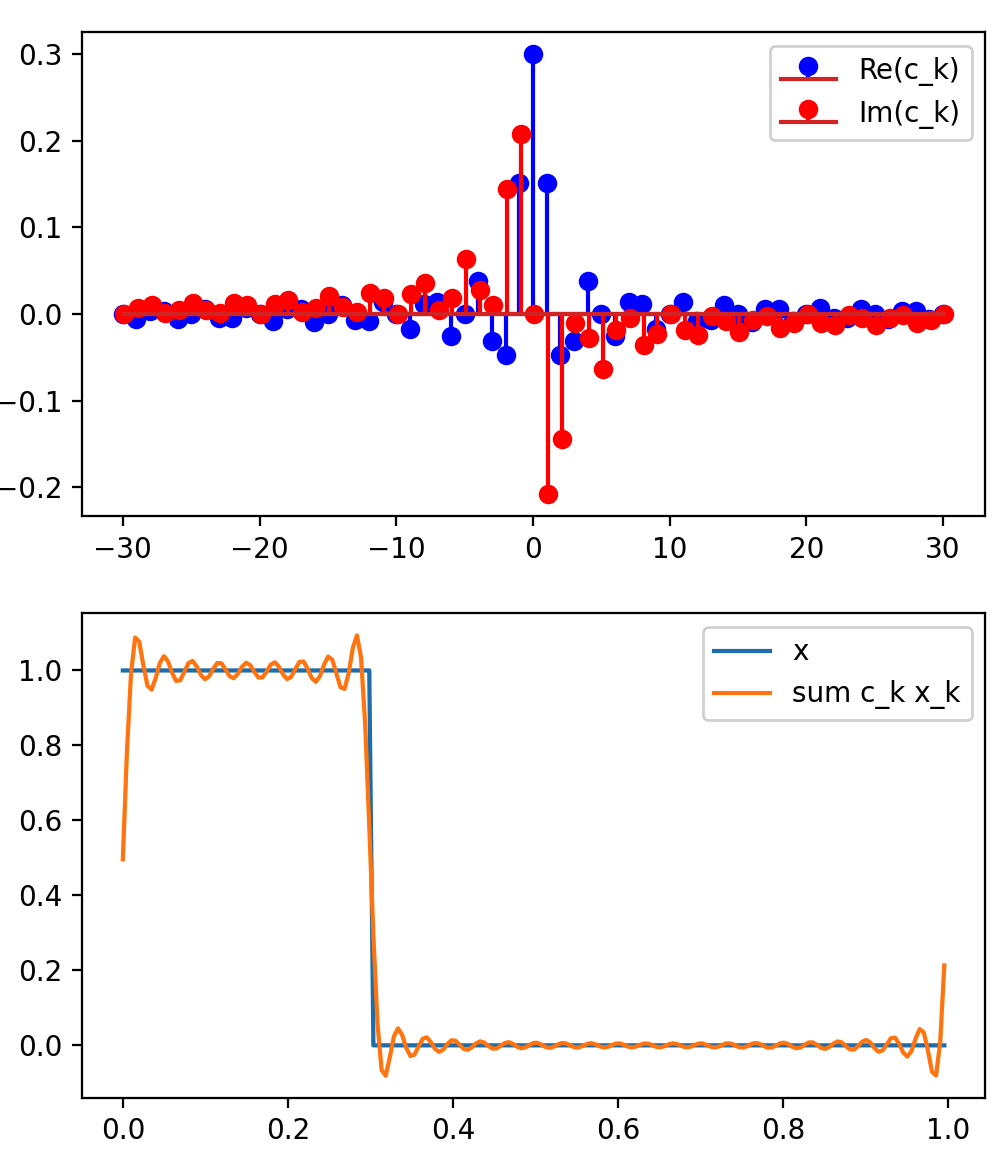
\includegraphics[width=\textwidth]{code/fourier_series.png}
    \end{minipage}
    \codecaption{dsv/code/fourier_series.py}{Berechnung und Darstellung von \eqref{eq:fourier:fourier_series}}\label{py:fourier_series}
\end{listing}

In \Cref{py:fourier_series} wird eine Rechteckfunktion $\Rect_{[0,T]}$ in ihre Fourier-Reihe entwickelt.
In diesem Fall m"ussen wir nat"urlich die Reihenentwicklung abbrechen, da kein $K_{\rm max}$ existiert, sodass $c[k] = 0$ f"ur $k > K_{\rm max}$.
Wir k"onnten die Reihe zwar analytisch ausrechnen, da wir jedes $x_k$ nur auf $[0,T]$ integrieren, also dem Bereich, auf dem die von uns definierte $\Rect_{[0,T]}$-Funktion Werte ungleich $0$ annimmt.
Der Einfachheit halber nutzen wir \texttt{scipy.integrate.quad}, was in der Lage ist numerische Integration relativ pr"azise durchzuf"uhren.

Es lohnt sich mit dem Wert von $K_{\rm max}$ zu experimentieren. 
Man sieht hierbei, dass gr"o"sere Werte von $K_{\rm max}$ an den Unstetigkeitsstellen $0$ und $T$ und in deren N"ahe nicht zu einer besseren "Ubereinstimmung der Fourierreiehe mit $x$ f"uhren.
Die Fourier-Reihe muss also nicht immer gegen $x$ konvergieren.
Im Falle von $\Rect_{[0,T]}$ ergibt sich das Problem genau aus dem Verhalten an $0$ und $T$ -- also Unstetigkeit, was ein generelles Problem bei der Entwicklung von Signalen in Fourier-Reihen darstellt.

Im oberen Plot von \Cref{py:fourier_series} sieht man auch, dass der Realteil der Koeffizienten $\Re{c[\cdot]}$ ein gerades diskretes Signal ist, also $c[k] = c[-k]$.
Der Imagin"arteil $\Im{c[\cdot]}$ hingegen ist ein ungerade Signal, also $c[k] = -c[-k]$\footnote{siehe \Cref{py:even_odd}}. 
Dies liegt daran, dass das Signal lediglich reelle Werte annimmt, weshalb die Symmetrie-Eigenschaften der $c[\cdot]$ allgemein f"ur reelle Signale gelten.

\begin{figure}
    \begin{center}
        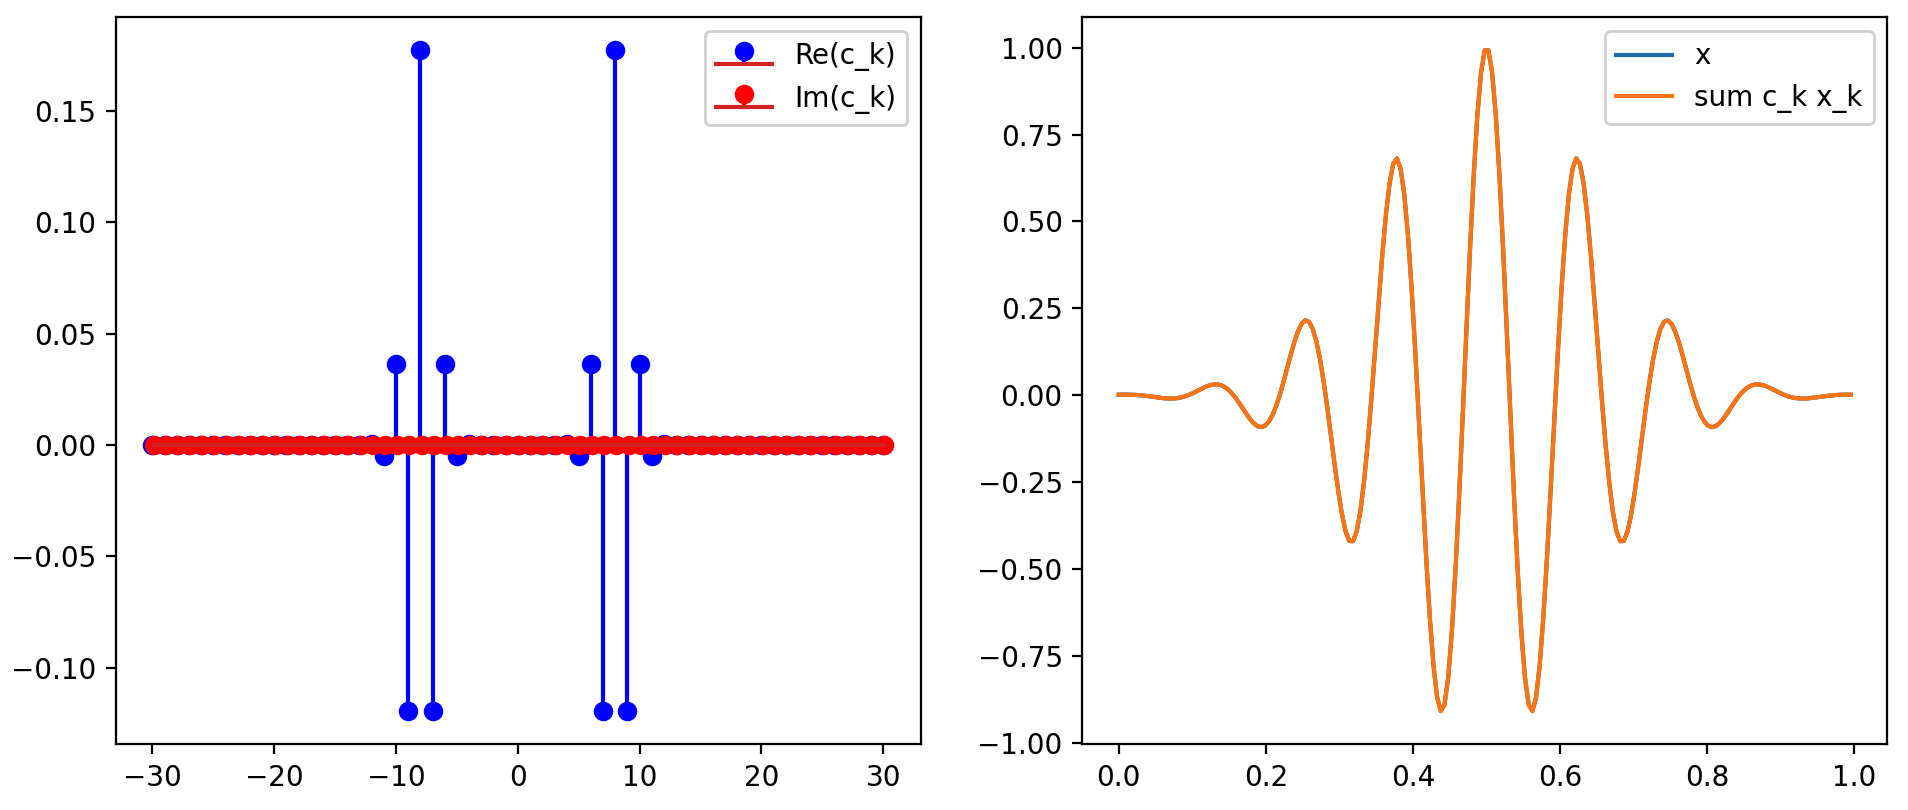
\includegraphics[width=0.8\textwidth]{code/fourier_series_1.png}

        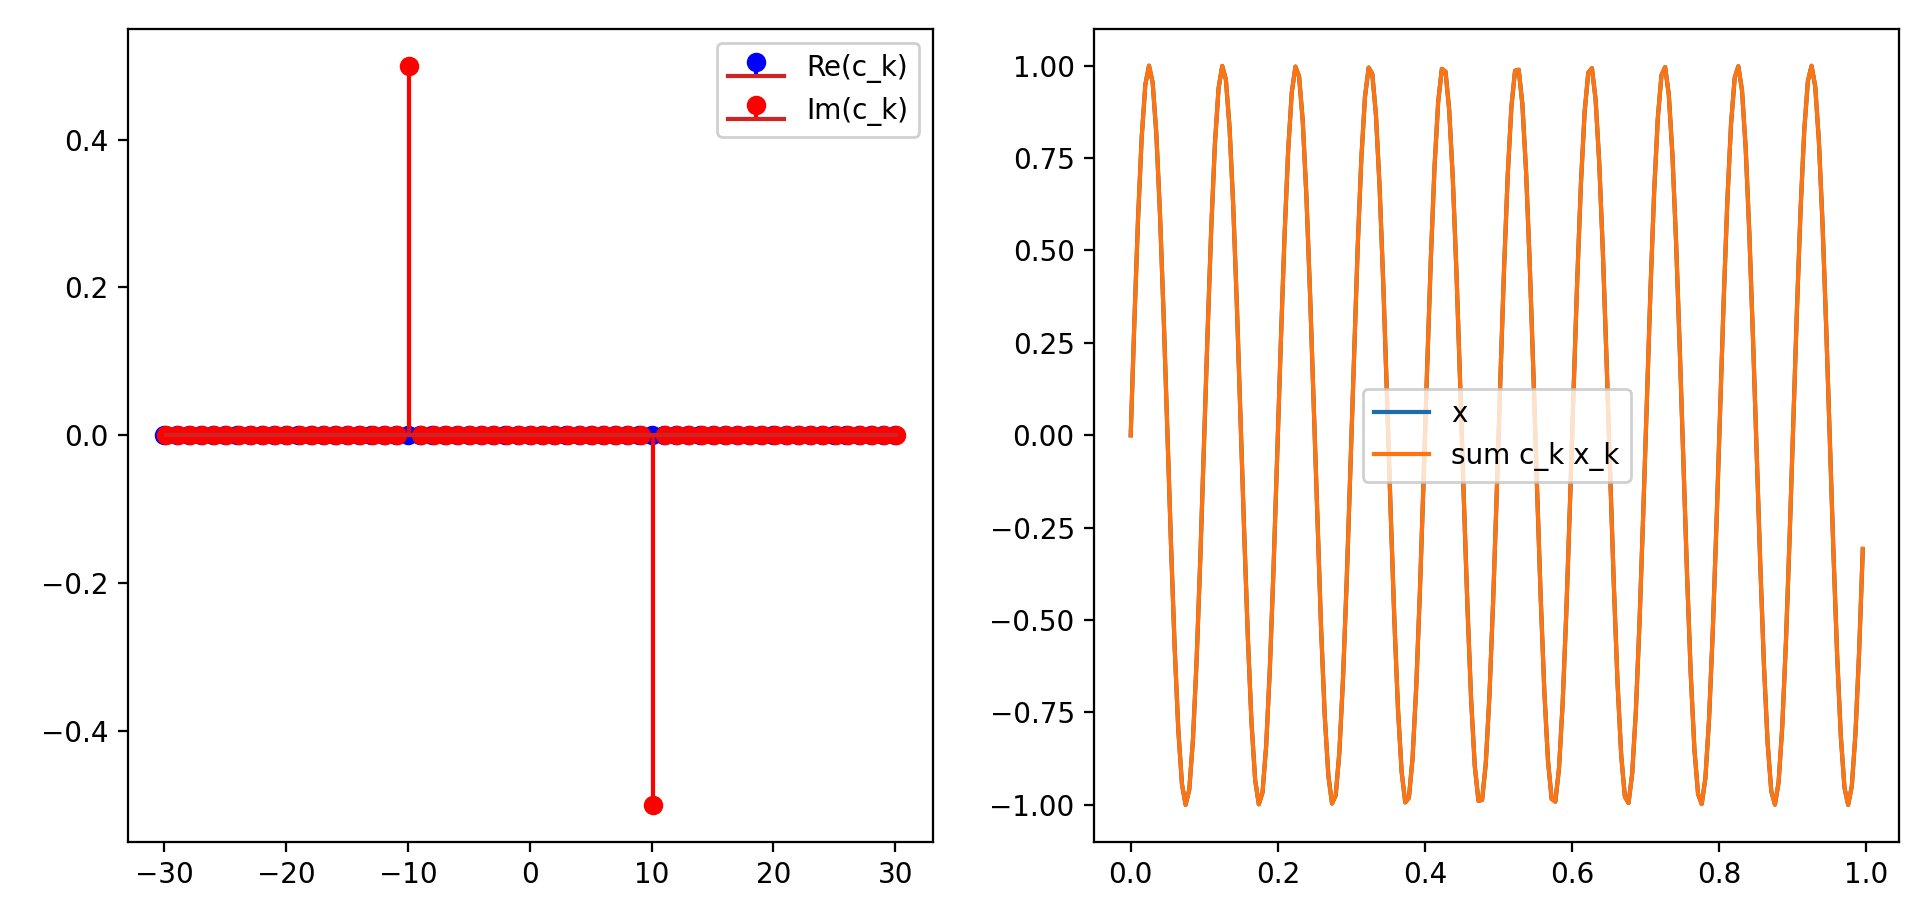
\includegraphics[width=0.8\textwidth]{code/fourier_series_2.png}
    \end{center}
    \caption{Mehr Versionen von \Cref{py:fourier_series}; Oben: $x(t) = \exp(-25(t-0.5)^2) \cos(16 \pi t)$; Unten: $x(t) = \sin(20 \pi t)$;}\label{fig:fourier:fourier_series}
\end{figure}

In \Cref{fig:fourier:fourier_series} sind noch mehr Eigenschaften der Fourier-Reihe deutlich gemacht.
Generell stellen wir fest, dass die beiden Signale jeweils gut durch eine endliche Fourier-Reihe approximiert werden k"onnen, da sie keine Unsteigkeiten aufweisen.
Im oberen Plot sieht man au"serdem, dass Achsen-Symmetrie des Signals $x$ dazu f"uhrt, dass die Imagin"arteile von $c[\cdot]$ verschwinden.
Wie man in \Cref{fig:fourier:fourier_series} unten sieht, ist es bei Anti-Symmetrie des Signals $x$ der Realteil von $c[\cdot]$, der verschwindet.
Dies liegt daran, dass der Realteil der $x_k$ eine gerade Funktion ist und der Imagin"arteil respektive eine ungerade Funktion.
Da wir in \Cref{py:even_odd} schon gesehen haben, dass ungerade und gerade Anteile eines Signals im Sinne von Skalarprodukten orthogonal sind, gilt dies auch f"ur die resultierenden Fourier-Koeffizienten.
In \Cref{fig:fourier:fourier_series} unten sieht man auch, dass man f"ur gewisse Signale die Fourier-Reihe direkt angeben kann.
Im Falle des Beispiels gilt n"amlich
\[
x(t) 
    = \sin(10 \cdot 2 \pi t) 
    = \frac{1}{2 \jmath} \left(
        \exp(10 \cdot 2 \pi t) - \exp(-10 \cdot 2 \pi t)
    \right) 
    = \frac{1}{2 \jmath} x_{10} - \frac{1}{2 \jmath} x_{-10}.
\]
Das hei"st, dass wir $x$ \emph{direkt} in seine Fourier-Reihe entwickelt haben, da wir es als Linearkombination der $x_k$ dargestellt haben.
Das hei"st es sind nur $x_{10}$ und $x_{-10}$ notwendig, um $x$ darzustellen und beide Koeffizienten haben ausschlie"slich imagin"are Anteile.

"Ahnlich wie bei der $z$-Transformation kann man also an der Fourier-Reihe Eigenschaften des Signals $x$ direkt ablesen, oder umgekehrt von Eigenschaften des Signals $x$ auf Eigenschaften der Fourier-Koeffizienten $c[\cdot]$ schlie"sen.
Au"serdem werden wir f"ur die noch folgenden Versionen der \gls{ft} sehr analoge Zusammenh"ange finden.

\subsubsection{Leichtungsdichte-Spektrum periodischer Signale}

Das Leichtungsdichtespektrum eines $T_0$-periodischen Signals $x: \R \rightarrow \C$ is gegeben durch
\begin{equation}\label{eq:fourier:period_psd}
P(x) = \frac{1}{T_0}\Int{0}{T_0}{\Abs{x(t)}^2}{t}
     = \frac{1}{T_0}\Int{0}{T_0}{x(t) x(t)^\ast}{t}
     = \frac{1}{T_0} \ScPr{x}{x}.
\end{equation}
Wir wollen nun $P(x)$ in Abh"angigkeit der Fourier-Koeffizienten $c[\cdot]$ berechnen.
Wir entwickeln also
\[
x(t) = \Sum{k \in \Z}{}{
    c_k \exp(\jmath 2 \pi k F_0 t)
}
\]
und setzen dies in $P$ ein, um
%
\begin{equation}\label{eq:fourier:series_parseval}
    \frac{1}{T_0}\Int{0}{T_0}{x(t) x(t)^\ast}{t}
        = \frac{1}{T_0}\Int{0}{T_0}{
            x(t) 
            \Sum{k \in \Z}{}{
                c_k^\ast \exp(-\jmath 2 \pi k F_0 t)
            }
        }{t}
        = \Sum{k \in \Z}{}{
            c_k^\ast 
            \frac{1}{T_0}\Int{0}{T_0}{
                x(t)
                \exp(-\jmath 2 \pi k F_0 t)
            }{t}
        }
        = \Sum{k \in \Z}{}{
            c_k^\ast c_k
        }
\end{equation}
%
als den \emph{Satz von Parseval}\footnote{\url{https://de.wikipedia.org/wiki/Satz\_von\_Parseval}} zu erhalten.
Die physikalische Interpretation ist, dass $\Abs{c[k]}$ der Leistung des Signals bei der Frequenz $k F_0$ entspricht.
Jeder Index $k$ hat also eine physikalische Gr"o"se, die mit ihm assoziiert ist.

Da nur die Frequenzen $k F_0$ f"ur $k \in \Z$ auftreten, also Frequenzen wie $0.1 F_0$ nicht vorhanden sind, sprechen wir von einem \emph{diskreten Spektrum}.
Es ergibt sich also direkt folgender wichtiger Zusammenhang: Periodische Signale im Zeitbereich besitzen ein \emph{diskretes} Spektrum.
Andersherum ergibt sich auch: Signale mit diskretem Spektrum sind periodisch.
Beide Argument ergeben sich aus der Fourier-Reihe.
Damit haben wir das duale Ergebnis zu \eqref{eq:spectrum_sampled} gefunden.
Dort f"uhrte Diskretisierung im Zeitbereich, also Sampling/Abtastung, zu einer Periodifizierung im Frequenzbereich.

\begin{listing}[ht]
    \noindent
    \begin{minipage}{0.51\textwidth}
        \strut\vspace*{-\baselineskip}\newline
        \inputminted[firstline=5, lastline=14]{python3}{code/period_psd.py}
    \end{minipage}%
    \begin{minipage}{0.48\textwidth}
        \strut\vspace*{-\baselineskip}\newline
        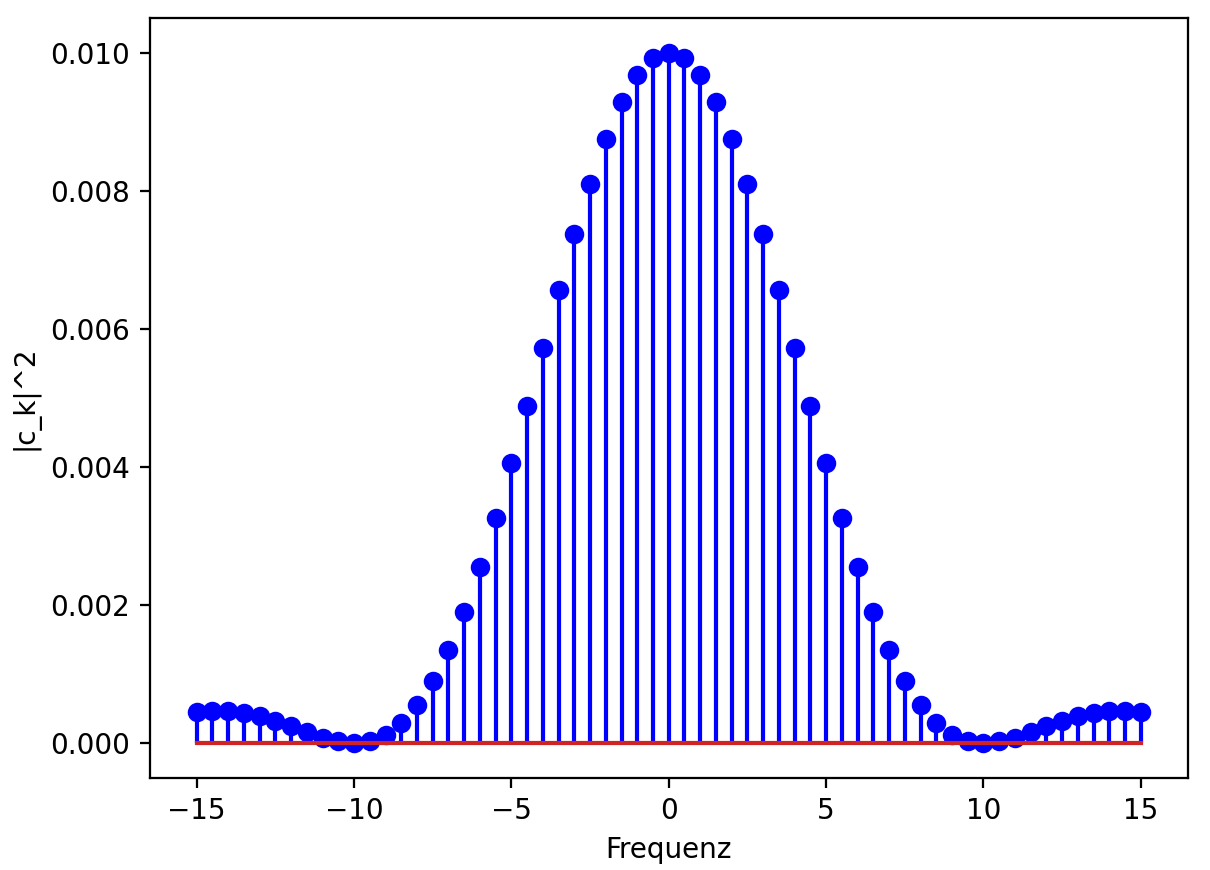
\includegraphics[width=\textwidth]{code/period_psd.png}
    \end{minipage}
    \codecaption{dsv/code/period_psd.py}{Modizifiertes \Cref{py:fourier_series} und Plot von $P$ im Frequenzbereich.}\label{py:period_psd}
\end{listing}

In \Cref{py:period_psd} zeigen wir eine Modifikation von \Cref{py:fourier_series}, in welcher wir $T_0 = 2$ setzen, also $F_0=1/2$ erhalten. 
Auf der Frequenzachse sehen wir, dass demnach diese f"ur $K_{\rm max} = 30$ also von $-15$ bis $+15$ reicht.
%
%
\FloatBarrier
\subsubsection{Fourier-Transformation von kontinuierlichen aperiodischen Signalen}
%
Um die Einschr"ankung auf periodische Signale zu vermeiden, nutzen wir die \acrlong{ft}, wie wir sie bereits in \eqref{eq:sampling:fourier_trafo} f"ur ein Signal $x : \R \rightarrow \C$ durch
\begin{equation}\label{eq:fourier:fourier_trafo}
    X(F) = \Int{-\infty}{+\infty}{x(t) \exp(-\jmath 2 \pi F t)}{t}
\end{equation}
definiert haben.
Im Unterschied zu \eqref{eq:fourier:fourier_series} integrieren wir nun "uber ganz $\R$, da sich das Signal nicht mehr periodisch wiederholt.
Aus diesem Grund ergibt sich auch ein \emph{kontinuierliches} Spektrum, da wir uns nicht mehr auf eine abz"ahlbare Menge von diskreten Frequenzen zur"uckziehen k"onnen.
Deshalb ergibt sich auch f"ur die Synthese des Signals, dass wir auch in diesem Fall integrieren anstatt summieren m"ussen, es gilt also
\begin{equation}\label{eq:fourier:inv_fourier_trafo}
    x(t) = \Int{-\infty}{+\infty}{X(F) \exp(\jmath 2 \pi F t)}{F}.
\end{equation}
Da sich f"ur die meisten Signale, die wir betrachten werden, Integration und Summation \q{"ahnlich} verhalten, finden wir auch die obigen Eigenschaften bez"uglich Symmetrien, etc., von \eqref{eq:fourier:fourier_series} wieder.

Es gibt aber eine Verbindung zur Fourier-Reihe, die wir im Folgenden kurz erl"autern wollen.
Nehmen wir an, es existiert ein $T > 0$, sodass $\Abs{x(t)} = 0$ f"ur alle $t$ mit $\Abs{t} > T$.
Dann k"onnen wir das Signal $x$ periodifizieren mit Periode $T$, indem wir
\[
x_p(t) = \Sum{k \in Z}{}{x(t - 2kT)}
\]
setzen.
Dies haben wir bereits in "ahnlicher Form in \eqref{eq:spectrum_sampled} gesehen. 
Dort hat es sich aber aus Berechnungen ergeben und hier \emph{setzen} wir diesen Zusammenhang explizit.
Dann k"onnen wir $x_p$ in seine Fourier-Reihe 
\[
x_p(t) = \Sum{k \in \Z}{}{c_k \exp(\jmath 2 \pi k t/T)}
\Text{mit}
T\,c_k = \Int{-T/2}{+T/2}{x_p(t) \exp(- \jmath 2 \pi k t/T)}{t}
    = \Int{-\infty}{+\infty}{x(t) \exp(- \jmath 2 \pi k t/T)}{t}
\]
entwickeln.
Aus der Definition in \eqref{eq:fourier:fourier_trafo} und der letzten Gleichung sehen wir, dass sich die Koeffizienten der Fourier-Reihe finden lassen durch
\begin{equation}\label{eq:fourier:c_k_fourier}
    c_k = \frac 1T X\left(\frac kT\right),
\end{equation}
diese sich also auch aus der Fourier-Transformation ablesen lassen.
Das hei"st, dass wir auch
\[
x_p(t) = \Sum{k \in \Z}{}{\frac 1T X\left(\frac kT\right) \exp(\jmath 2 \pi k t/T)}
       = \Sum{k \in \Z}{}{X\left(k \Delta F\right) \exp(\jmath 2 \pi k t \Delta F) \Delta F}
\]
schreiben k"onnen.
Dabei haben wir im letzten Schritt $1/T = \Delta F$ gesetzt.
Dies k"onnen wir intuitiv (aber nicht rigoros!) so interpretieren, dass im Falle von $T \rightarrow \infty$ gilt, dass $\Delta F \rightarrow 0$.
Je l"anger der Bereich der Funktion $x$, auf welchem gilt $x \neq 0$, desto kleiner $\Delta F$.
Der nicht-periodische Fall $T = \infty$ ergibt sich also als Grenzfall, bei welchem obige Summation zu einer Integration wird und $\Delta F$ zu einem $\mathrm{d}F$.
Man kann die \acrlong{ft} also als Grenzfall der Fourier-Reihe f"ur $T \rightarrow \infty$ betrachten.
%
%
\subsubsection{Leistungsdichte-Spektrum aperiodischer Signale}
%
Analog zum Satz von Parseval f"ur periodische Signale in \eqref{eq:fourier:series_parseval} k"onnen wir auch hier wieder definieren und folgern, dass
\begin{equation}
E(x) = \Int{-\infty}{+\infty}{\Abs{x(t)}^2}{t}
     = \Int{-\infty}{+\infty}{\Abs{X(F)}^2}{F}
\end{equation}
auch wieder ein Parseval Theorem f"ur die \acrlong{ft} ergibt, was aber in diesem Fall als Plancherel Theorem\footnote{\url{https://en.wikipedia.org/wiki/Plancherel_theorem}} genannt wird.

Andererseits kann man $X$ auch in Betrag und Phase zerlegen, da es im Allgemeinen eine komplexe Gr"o"se ist, also
\[
X(F) = \Abs{X(F)} \exp(\jmath \angle(X(F))).
\]
Man nennt dann $\Abs{X(F)}^2$ das \emph{Leistungsdichte-Spektrum} von $x$.

\begin{listing}[ht]
    \noindent
    \begin{minipage}{0.51\textwidth}
        \strut\vspace*{-\baselineskip}\newline
        \inputminted[firstline=6, lastline=45]{python3}{code/fourier_trafo.py}
    \end{minipage}%
    \begin{minipage}{0.48\textwidth}
        \strut\vspace*{-\baselineskip}\newline
        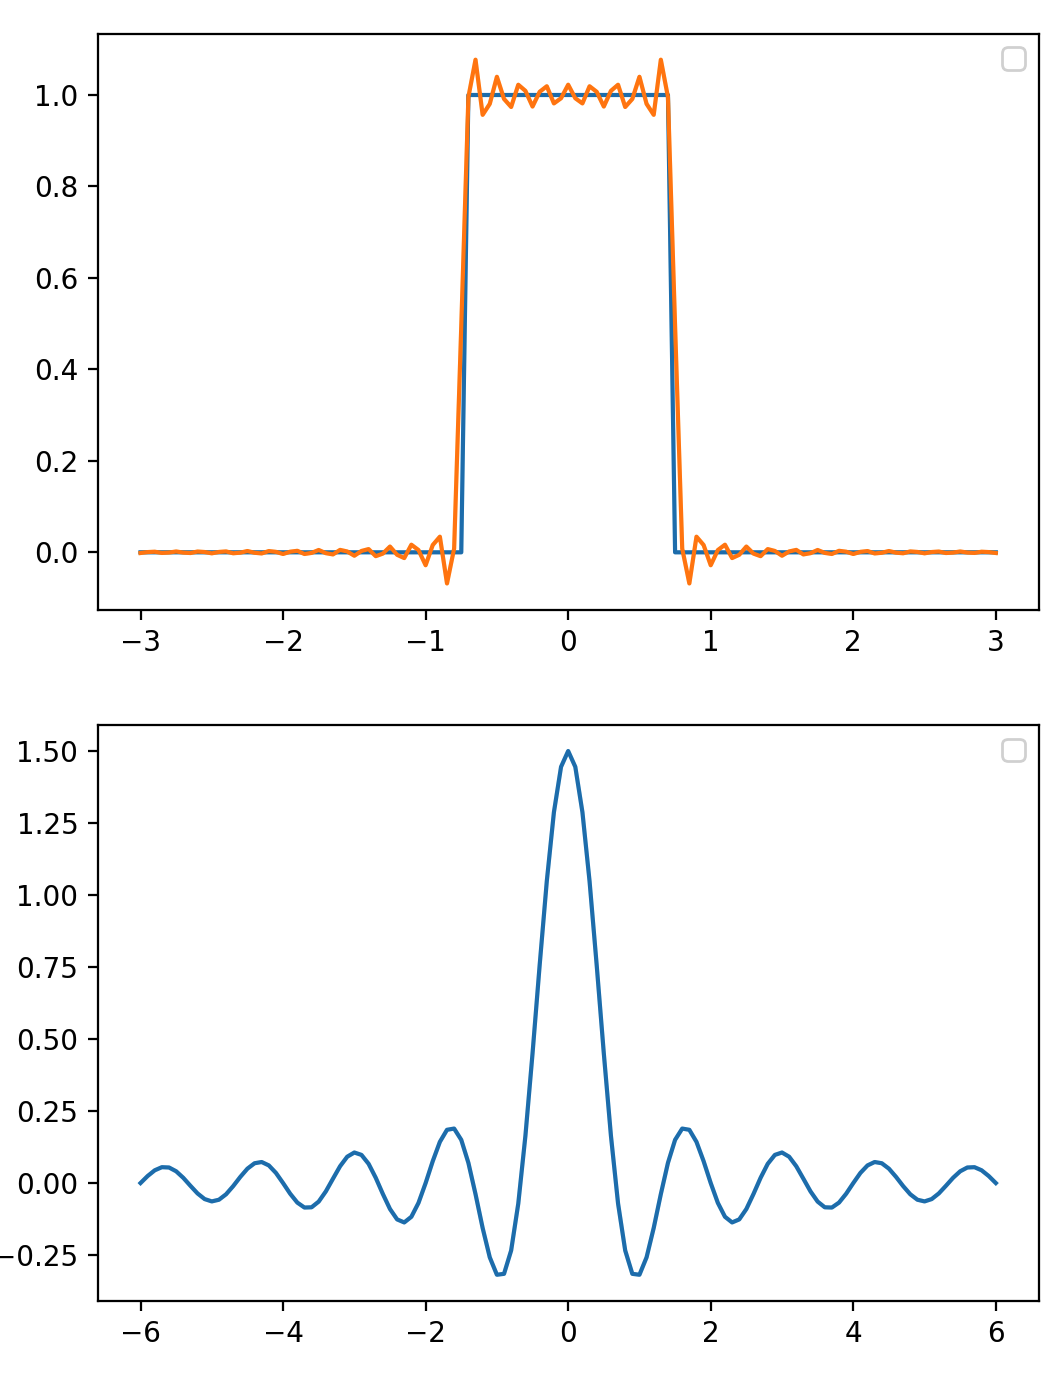
\includegraphics[width=\textwidth]{code/fourier_trafo.png}
    \end{minipage}
    \codecaption{dsv/code/fourier_trafo.py}{Berechnung und Darstellung von \eqref{eq:fourier:fourier_trafo}}\label{py:fourier_trafo}
\end{listing}

In \Cref{py:fourier_trafo} zeigen wir das Vorgehen zur Fourier-Analyse mittels numerischer Integration.
Es ist hier anzumerken, dass wir \q{nur} die Funktion \texttt{rect} definieren m"ussen und der Rest, also die Funktionen \texttt{kernel}, \texttt{analyse} und \texttt{synthese} unabh"angig hiervon sind.
Wir haben hier ein \namecref{py:fourier_trafo}, welches sich Methoden der Funktionalen Programmierung bedient.
Die Funktionen texttt{analyse} und \texttt{synthese} haben als Eingabewert die entweder die Funktion, oder die \acrlong{ft} einer Funktion.
Au"serdem liefern sie als Ausgabewert wieder \emph{Funktionen}, die wir einfach \q{aufrufen} k"onnen.
%
\subsection{Fourier-Transformation diskreter Signale}\label{sec:fourier:disc}
%
Wir n"ahern uns langsam der Fourier-Analyse von diskreten Signalen.
Schlie"slich wollen wir etwaige spektrale Analysen und dergleichen im Digitalen durchf"uhren, um die Vorz"uge von digitalen Rechenwerken dabei nutzen zu k"onnen.
Die vorher eingef"uhrten Transformationen sind zwar hilfreich f"ur theoretische Argumentation, wie beispielsweise beim Sampling-\Cref{stm:sampling_theorem}. 
Deshalb wenden wir uns nun der spektralen Analyse von diskreten Signalen zu.
Wir werden aber im Verlauf auch wieder "ahnliche Zusammenh"ange wie in \eqref{eq:fourier:c_k_fourier} finden.
%
\subsubsection{Fourier-Transformation diskreter periodischer Signale}\label{sec:fourier:disc_period}
%
Wir beginnen mit diskreten Signalen, die gleichzeitig periodisch sind, also ein $N$ existiert, sodass
\[
x[n] = x[n+kN] \Text{f"ur alle} n,k \in \Z 
\]
gilt.
Aus vorherigen Diskussionen in \Cref{sec:sampling} wissen wir einerseits, dass diskrete Signale ein periodisches Spektrum auf $(0,1)$ besitzen.
Andererseits wissen wir aus \Cref{sec:fourier:cont:period}, dass periodische Signale ein \emph{diskretes} Spektrum besitzen.
Wir finden also nun intuitiv, dass das Spektrum von diskreten periodischen Signalen \emph{ebenfalls} diskret und periodisch ist.
Denken wir zur"uck an \Cref{sec:sampling:disc_sin} so haben wir bereits alles Notwendige betrachtet.
Ein $N$-periodisches diskretes Signal ergibt sich aus der Linearkombination der diskreten Signale $x_k[\cdot] : \Z \rightarrow \C$ definiert durch
\[
x_k[n] = \exp\left(\jmath 2 \pi \frac k N n \right) \Text{mit} k = 0, \ldots, N-1.
\]
Das hei"st, f"ur $x[\cdot]$ setzen wir mit
\[
x[\cdot] = \Sum{k = 0}{N-1}{c[k] x_k[\cdot]}
\]
an.
Damit sind bereits beide Eigenschaften des Spektrums \q{eingepreist}.
Denn man erkennt in den $x_{k}[\cdot]$ die vorher erw"ahnte \emph{zweifache} Periodizit"at wieder, weil sowohl $x_{k+N}[\cdot] = x_{k}[\cdot]$ f"ur alle $k$ als auch $x_k[n+N] = x_k[n]$ f"ur alle $n$ gilt.

Es ist nun unser Ziel f"ur gegebene Werte $x[n]$ von $x[\cdot]$ die Werte des \emph{ebenfalls periodischen und diskreten} Signals $c[\cdot]$ zu bestimmen.
Dies verl"auft ganz analog zu \Cref{sec:fourier:cont:period}.
Wir definieren das Skalarprodukt $\ScPr{\cdot}{\cdot}$ f"ur $N$-periodische und diskrete Signale via
\[
\ScPr{x_1[\cdot]}{x_2[\cdot]} 
    = \Sum{n = 0}{N-1}{x_1[n] x_2[n]^\ast}.
\]
Das hei"st, dass wir periodisches Signal $x[\cdot]$ mit dem \emph{endlich-dimensionalen} Vektor $\bm x \in \C^{N}$ identifizieren, wir setzen also die Eintr"age des Vektors als $\bm x_i = x[i-1]$.
Dann k"onnen wir auch f"ur das entsprechende Skalarprodukt der Vektoren $\bm x_{1,2} \in \C^N$
\[
\ScPr{\bm x_1}{\bm x_2} 
    = \left(\bm x_2^\ast\right)^\trans \cdot \bm x_1 
    = \bm x_2^\herm \cdot \bm x_1
\]
schreiben.
Analog identifizieren wir die periodische und diskrete Sequenz $c[\cdot]$ mit dem Vektor $\bm c \in \C^N$.

Wie in \Cref{sec:fourier:cont:period} m"ussen wir nur 
\[
\ScPr{\bm x_k}{\bm x_\ell} 
    = \Sum{i=0}{N-1}{
        x_k[i] x_\ell[i]^\ast
    }
    = \Sum{i=0}{N-1}{
        \exp\left(\jmath 2 \pi \frac{i(k-l)}{N} \right)
    }
    = \begin{cases}
        N \Text{falls} k = \ell \\
        \frac{
            1 - \exp\left(\jmath 2 \pi \frac{(k-l)}{N} \right)^N   
        }{
            1 - \exp\left(\jmath 2 \pi \frac{(k-l)}{N} \right)
        } \Text{sonst}
    \end{cases}
    = \begin{cases}
        N \Text{falls} k = \ell \\
        0 \Text{sonst}
    \end{cases}
\]
berechnen.
Hierbei nutzen wir, dass $\exp(\jmath 2 \pi k) = 1$ f"ur alle $k \in \Z$.
Wie in \Cref{sec:fourier:cont:period} finden wir, dass also gilt $\ScPr{\bm x_k}{\bm x_\ell} = 0$, falls $k \neq \ell$ und $\ScPr{\bm x_k}{\bm x_k} = N$.
Damit ergibt sich bei Anwendung auf das eigentliche Signal $\bm x$ f"ur den Vektor $\bm c$, dass
\[
\ScPr{\bm x}{\bm x_\ell}
    = \ScPr{\Sum{k=1}{N}{\bm c_k \bm x_k}}{\bm x_\ell}
    = \Sum{k=1}{N}{\bm c_k \ScPr{\bm x_k}{\bm x_\ell}}
    = N \bm c_\ell
\Rightarrow
\bm c_\ell = \frac{1}{N}\ScPr{\bm x}{\bm x_\ell}.
\]
Zusammenfassend, kann man also sagen, dass sich folgende Analyse- und Synthesegleichungen ergeben:
\begin{equation}\label{eq:fourier:disc_analys_synth}
    x[n] = \Sum{k = 0}{N-1}{c[k]\exp(\jmath 2 \pi k n/N)}, \Text{und}
    c[k] = \frac{1}{N}\Sum{n = 0}{N-1}{x[n]\exp(-\jmath 2 \pi k n/N)}.
\end{equation}
In Vektorschreibweise l"asst sich der erste Teil durch
\begin{equation}\label{eq:fourier:disc_analys_synth_vec}
    \bm x = \Sum{k = 0}{N-1}{\ScPr{\bm x}{\bm x_k} \bm x_k}
\end{equation}
ausdr"ucken.

Weiterhin, k"onnen wir eine Matrix $\bm F_N \in \C^{N \times N}$ definieren, deren $k$-te Spalte den Vektor $\bm x_k$ beinhaltet.
Wir definieren also 
\[
\bm F_N = \left[
    \bm x_1, \ldots, \bm x_k, \ldots, \bm x_N 
\right]
\]
Dann k"onnen wir noch einen Schritt weitergehen und sehen, dass
\[
\bm c = \frac{1}{N} \bm F_N^\herm \bm x, \Text{und} \bm x = \bm F_N \bm c
\]
gilt.
Das hei"st, dass sich Fourier-Analyse und Fourier-Synthere von diskreten und periodischen Signalen durch eine Matrix-Vektor-Multiplikation durchf"uhren l"asst!
Das sind erst einmal gute Nachrichten, denn damit wissen wir, dass digitale Rechenwerke sehr gut darin sind, diese Transformation durchzuf"uhren.
Die hier vorgestellte Transformation nennen wir \gls{dft} und oft definiert man ein diskretes Signal $X[\cdot]$ durch
\begin{equation}
    X[k] = \frac{1}{N}\Sum{n = 0}{N-1}{x[n]\exp(-\jmath 2 \pi k n/N)} = c[k] = \bm c_k
\end{equation}
und nennt dieses dann die \gls{dft} von $x[\cdot]$.
Es ist anzumerken, dass der Vorfaktor $N^{-1}$ in manchen Lehrb"uchern oder Ver"offentlichungen auch bei der Synthese anstatt der Analyse auftaucht, oder aber \emph{beide} Gleichungen erhalten einen Faktor $N^{-1/2}$.

In \Cref{py:dft_1} zeigen wir ein einfaches Beispiel f"ur $x[\cdot] = u[\cdot] - u[\cdot-k]$.
Au"serdem zeigen wir auch die beiden Berechungsmethoden der $c[\cdot]$ -- einerseits mit der Definition und andererseits "uber ein Matrix-Vektor-Produkt.
%
\begin{listing}[ht]
    \noindent
    \begin{minipage}{0.51\textwidth}
        \strut\vspace*{-\baselineskip}\newline
        \inputminted[firstline=5, lastline=23]{python3}{code/dft_1.py}
    \end{minipage}%
    \begin{minipage}{0.48\textwidth}
        \strut\vspace*{-\baselineskip}\newline
        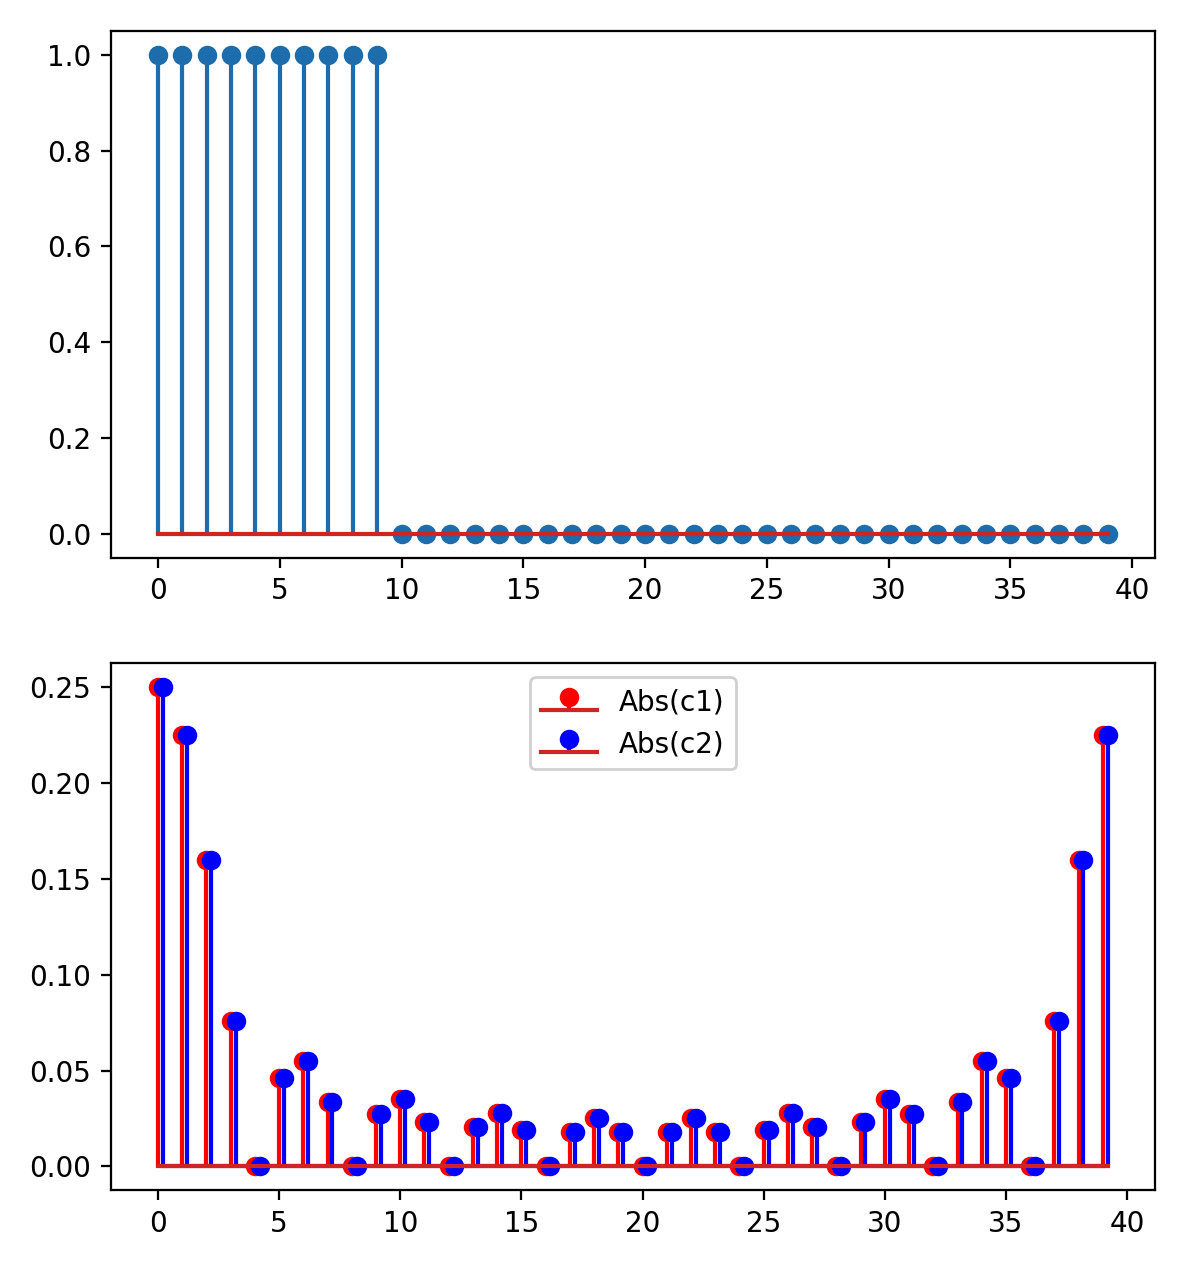
\includegraphics[width=\textwidth]{code/dft_1.png}
    \end{minipage}
    \codecaption{dsv/code/dft_1.py}{Berechnung und Darstellung von \eqref{eq:fourier:disc_analys_synth}}\label{py:dft_1}
\end{listing}
%
\subsubsection{Leichtungsdichte-Spektrum diskreter periodischer Signale}\label{sec:fourier:disc_period_power}
%
Da periodische Signale keine endliche Energie besitzen, betrachten wir die durchschnittliche Leistung "uber eine Periode.
Wir betrachten also f"ur ein $N$-periodisches Signal $x[\cdot]$ das Funktional
\begin{equation}
    P(x[\cdot]) = \frac{1}{N}\Sum{i=0}{N-1}{\Abs{x[n]}^2}.
\end{equation}
Dann k"onnen wir ganz analog zu vorher wieder herleiten, dass f"ur
\[
x[\cdot] = \Sum{i=0}{N-1}{c[k] x_k[\cdot]}
\]
und dessen Leistung gilt, dass
\[
P(x[\cdot]) = \Sum{i=0}{N-1}{\Abs{c[k]}^2}.
\]
Also auch hier finden wir wieder, dass sich die durchschnittliche Leistung einer Periode im Zeitbereich auf die Leistung einer Periode im Frequenzbereich "ubertr"agt.
Auch hier k"onnen wir die Folge $\Abs{c[\cdot]}^2$ als Leistungsdichte-Spektrum interpretieren.
\FloatBarrier
%
\subsubsection{Fourier-Transformation diskreter aperiodischer Signale}\label{sec:fourier:disc_aperiod}
%
Wiederum analog zu \Cref{sec:fourier:cont} ben"otigen wir noch eine Transformation f"ur diskrete Signale, die keine Periodizit"at aufweisen.
Hierzu definieren wir die zugeh"orige Fourier-Transformation, die wir \gls{dtft} nennen, durch
\begin{equation}\label{eq:fourier:dtft}
    X(f) = \Sum{n \in \Z}{}{x[n] \exp(-\jmath 2 \pi f n)},
\end{equation}
genau wie in \Cref{sec:sampling} bei der Herleitung von \eqref{stm:sampling_theorem}.
Im Unterschied zur \q{analogen} Fourier-Transformation \eqref{eq:fourier:fourier_trafo} sehen wir, dass $X$ nur f"ur Frequenzen $f \in (0,1]$ definiert ist, da das diskrete Signal $x_f[n] = \exp(\jmath 2 \pi f n)$ periodisch in $f$ ist.
Es gilt also $x_{f + k}[\cdot] = x_{f}[\cdot]$ f"ur alle $k \in \Z$.
Dies \q{passt} auch zur Natur von diskreten Signalen, da deren Frequenzbereich \emph{immer} periodisch sein muss.

Wir k"onnen nun f"ur die inverse Transformation \eqref{eq:fourier:dtft} mit \eqref{eq:fourier:fourier_series} vergleichen. 
Bis auf das Vorzeichen in der Funktion $\exp()$ gleicht \eqref{eq:fourier:dtft} einer Fourier-Reihe der periodischen Funktion $X$.
In der Tat, k"onnen wir die Folge $x[\cdot]$, also das urspr"ungliche Signal, als Fourier-Koeffizienten der \gls{dtft} $X$ durch
\begin{equation}\label{eq:fourier:idtft}
    x[n] = \Int{-1/2}{+1/2}{X(f)\exp(\jmath 2 \pi f n)}{f}
\end{equation}
wiederfinden.
Diese Synthese-Operation nennen wir dann \gls{idtft}.
Es ist wiederum anzumerken, dass die \gls{dtft} \q{nur} ein theoretisches Werkzeug ist, da sich im Allgemeinen die unendliche Summe in \eqref{eq:fourier:dtft} praktisch nicht realisieren l"asst, genauso wenig wie deren Resultat, eine kontinuierliche Funktion.

In \Cref{py:dtft} zeigen wir dennoch, wie man die \gls{dtft} einer aperiodischen Folge approximieren kann.
Wir studieren hierzu das Signal
\[
x[n] = \begin{cases}
    \frac{\omega}{\pi} \Text{f"ur} n = 0,\\
    \frac{\omega}{\pi} \frac{\sin(\omega n)}{\omega n} \Text{sonst}.
\end{cases}
\]
Dessen analytisch bestimmte \gls{dtft} $X$ ist
\[
X(f) = \Rect(f/(2 \pi \omega)),
\]
welche wir durch eine endliche Summe "uber die von uns verf"ugbaren Werte von $x[\cdot]$ bestimmen.

Nun treten hierbei mehrere Effekte zutage.
%
\begin{itemize}
\item Die Approximation der \gls{dtft} mittels des \q{abgeschnittenen} Signals $x$ stimmt noch nicht sehr gut mit der analytischen L"osung "uberein. 
Ver"andert man den Wert der Variable $N$ im Skript, tritt dieser Effekt st"arker oder schw"acher zutage.
\item Auch bei Erh"ohung von $N$ stellt sich immernoch keine Konvergenz von $X_{\rm approx}$ gegen $X_{\rm true}$ ein.
Dies liegt daran, dass die \gls{dtft} von $x[\cdot]$ nicht konvergiert, wie wir in \Cref{py:fourier_series} bereits gesehen hatten.
Diesen Effekt bezeichnet man allgemein als Gibbssches Ph"anomen\footnote{\url{https://en.wikipedia.org/wiki/Gibbs_phenomenon}}.
\item Augenscheinlich ist es besser die \gls{idtft} aus $X_{\rm approx}$ zu berechnen, als aus $X_{\rm true}$. Doch dies liegt legidlich daran, dass die numerische Integration der $\Rect$-Funktion nicht genau genug ist.
Erh"oht man die Anzahl der Punkte im Array \texttt{F}, dann stimmen im dritten Plot die drei Graphen besser "uberein.
\end{itemize}
%
\begin{listing}[ht]
    \noindent
    \begin{minipage}{0.51\textwidth}
        \strut\vspace*{-\baselineskip}\newline
        \inputminted[firstline=5, lastline=48]{python3}{code/dtft.py}
    \end{minipage}%
    \begin{minipage}{0.48\textwidth}
        \strut\vspace*{-\baselineskip}\newline
        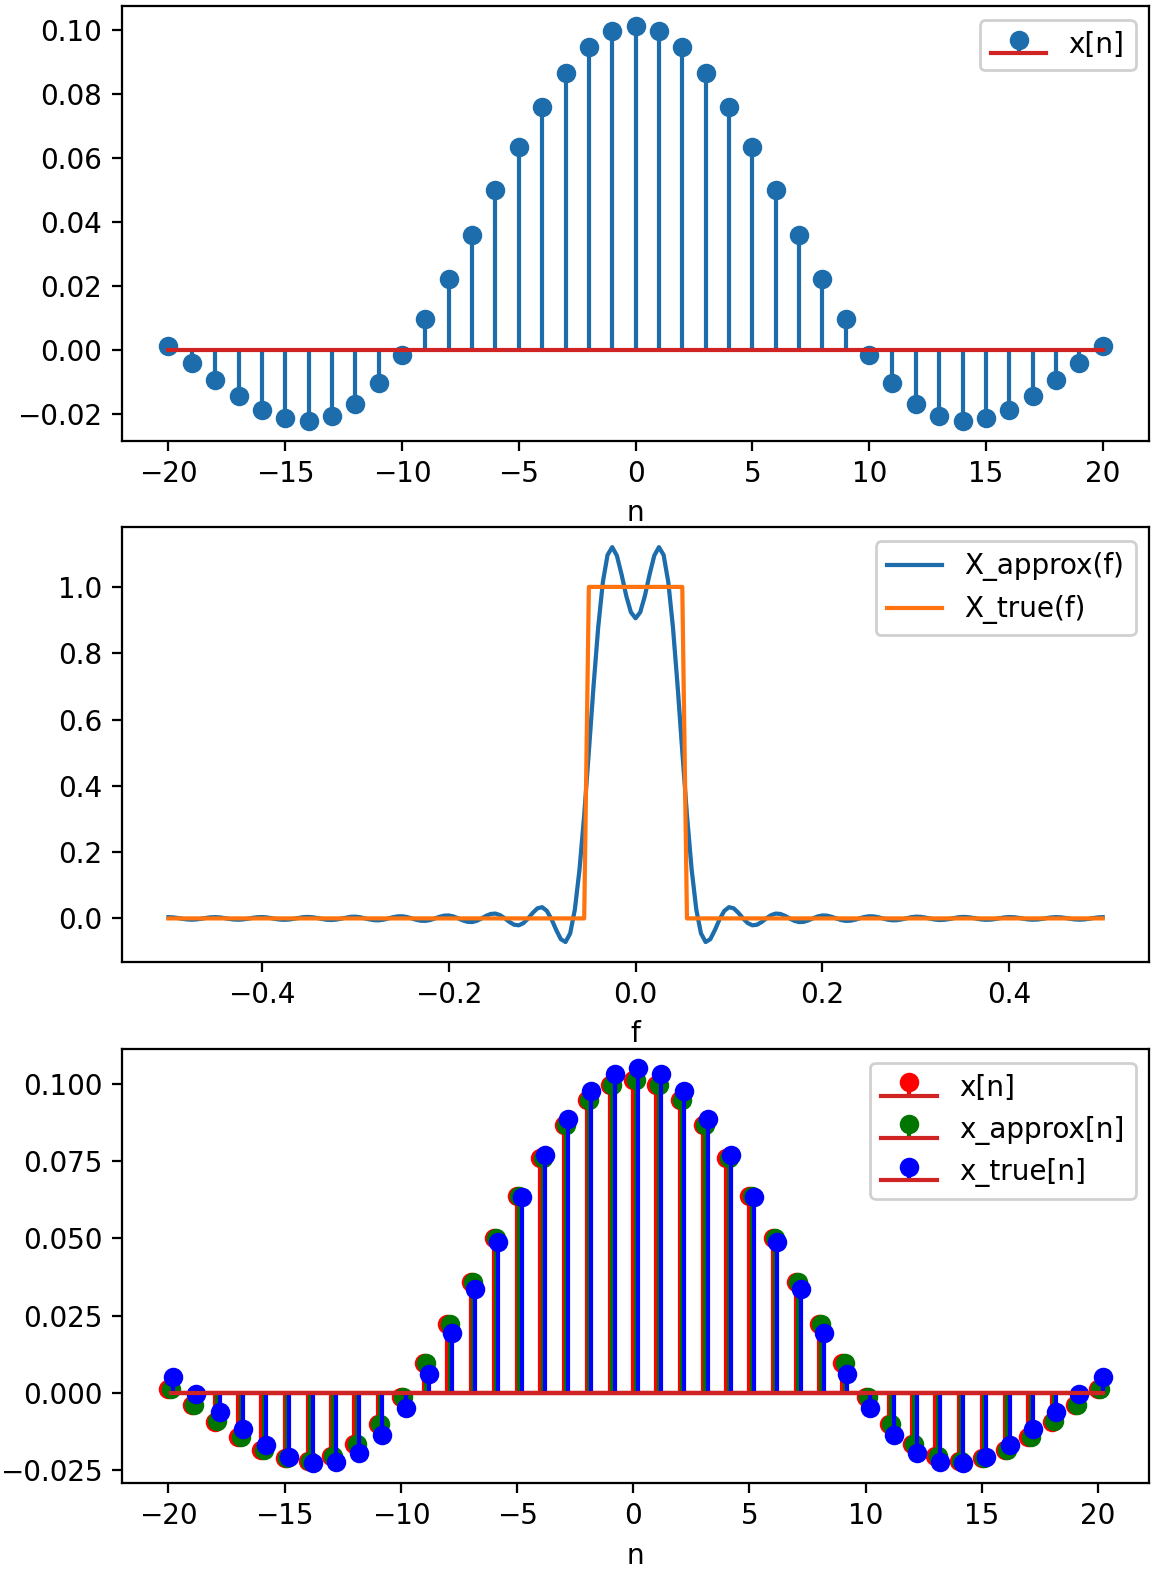
\includegraphics[width=\textwidth]{code/dtft.png}
    \end{minipage}
    \codecaption{dsv/code/dtft.py}{Berechnung und Darstellung von \eqref{eq:fourier:dtft}}\label{py:dtft}
\end{listing}
%
\FloatBarrier
\subsubsection{Leichtungsdichte-Spektrum diskreter aperiodischer Signale}\label{sec:fourier:disc_aperiod_power}
%
Die Energie eines diskreten Signals haben wir in \eqref{eq:disc_sig_energy} durch
\[
\mathcal{E}(x[\cdot]) = \Sum{n \in \Z}{}{\Abs{x[n]}^2} 
\]
definiert.
Wiederum k"onnen wir uns "uberlegen, dass dann f"ur die \gls{dtft} $X$ gilt, dass
\[
\mathcal{E}(x[\cdot]) = \Int{-1/2}{+1/2}{\Abs{X(f)}^2}{f}.
\]
Schlussendlich bezeichnet man dann
\[
S_{xx}(f) = \Abs{X(f)}^2
\]
als das Leichtungsdichte-Spektrum des Signals $x[\cdot]$.
In manchen Anwendungen ist es auch wieder sinnvoll Betrag und Phase von $X(f)$ zu analysieren.
%
\subsection{Eigenschaften der Fourier-Transformationen}\label{sec:fourier:proper}
%
Nachdem wir nun die notwendigen Definitionen gesammelt haben, wollen wir uns einige wichtige Eigenschaften der definierten Transformationen ansehen und eventuell auch f"ur \q{praktische} Dinge verwenden.
%
\subsubsection{Beziehung der Fourier-Transformationen und der \texorpdfstring{$z$}{z}-Transformation}
%
Wie wir in \cref{sec:ztrafo} gesehen haben, ist die $z$-Transformation f"ur ein diskretes Signal $x[\cdot]$ definiert durch
\[
X_{\z}(z) = \Sum{n \in \Z}{}{x[n]z^{-n}} \Text{mit \gls{roc}} r_2 < \Abs{z} < r_1.
\]
Wenn wir nun $z$ in Polarform $z = r \exp(\jmath 2 \pi f)$ ausdr"ucken und annehmen, dass $r_2 < r , r_1$, dann sehen wir, dass die $z$-Transformation von $x[\cdot]$ nichts anderes ist als die \gls{dtft} von $x[n] r^{-n}$ ist.
Mit anderen Worten ist die $z$-Transformation an einer Stelle $z=r \exp(\jmath 2 \pi f)$ die \gls{dtft} $X$ eines Signals gewichtet mit der Folge $w[n] = r^{-n}$ an der Stelle $f$.
Ist nun $1 \in \gls{roc}$ (und damit der gesamte Einheitskreis der komplexen Ebene), dann gilt
\begin{equation}\label{eq:fourier:ztrafo}
    X_{\z}(\exp(\jmath 2 \pi f)) = X(f)
\end{equation}
Wir haben uns zwar bis jetzt wenig Gedanken "uber die Existenz der Fourier-Transformation gemacht, doch hier finden wir einen Hinweis. 
Die \gls{dtft} existiert, beziehungsweise \emph{konvergiert}, falls $1 \in \gls{roc}$.
Da die \q{Form} der \gls{roc} immer kreisf"ormig ist, ist die gleichbedeutend mit der Tatsache, dass sich der Einheitskreis der komplexen Ebene in der \gls{roc} befindet.
Au"serdem kann man auch eine Fourier-Analyse von \gls{lti}-Systemen betreiben. 
Dann ist die \gls{bibo}-Stabilit"at von einem solchen System "aquivalent zur Tatsache, dass der Einheitskreis in der \gls{roc} liegt.
Wie wir gerade gesehen haben, folgt dann auch, dass \gls{bibo}-Stabilit"at ebenfalls durch die \emph{Existenz} der \gls{dtft} charakterisiert wird.
%
\begin{listing}[ht]
    \noindent
    \begin{minipage}{0.51\textwidth}
        \strut\vspace*{-\baselineskip}\newline
        \inputminted[firstline=5, lastline=46]{python3}{code/dtft_z.py}
    \end{minipage}%
    \begin{minipage}{0.48\textwidth}
        \strut\vspace*{-\baselineskip}\newline
        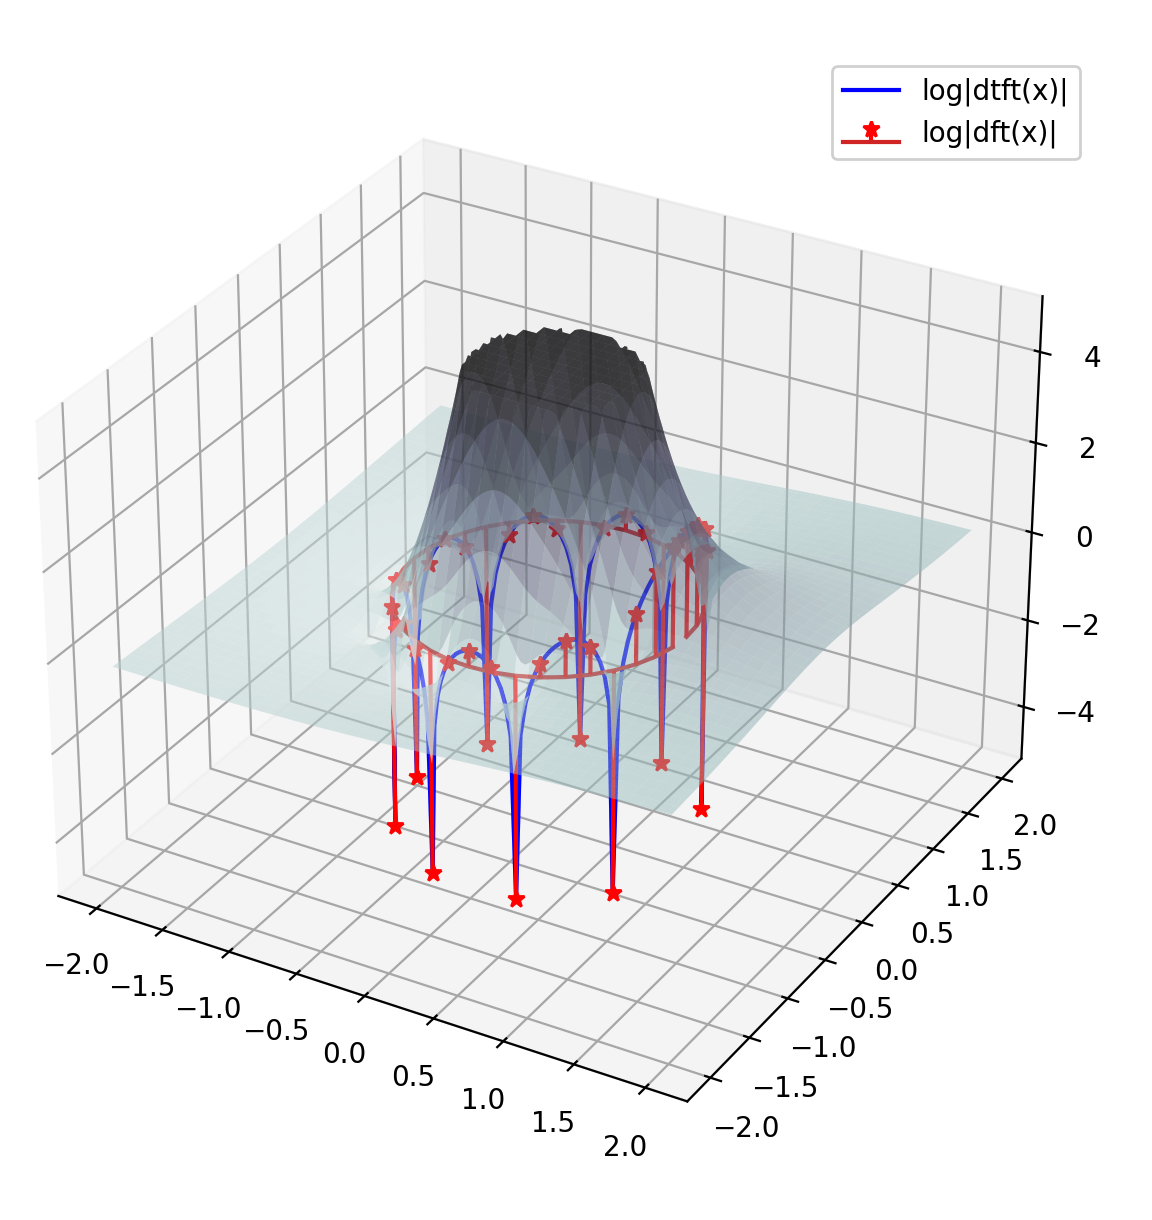
\includegraphics[width=\textwidth]{code/dtft_z.png}
    \end{minipage}
    \codecaption{dsv/code/dtft_z.py}{Berechnung und Darstellung von \eqref{eq:fourier:ztrafo}}\label{py:dtft_z}
\end{listing}

In \Cref{py:dtft_z} zeigen wir diesen Zusammenhang f"ur das gleiche Signal, wie in \Cref{py:dft_1}, interpretieren es hier aber einmal als aperiodisches Signal bei der Berechnung der \gls{dtft} und als periodisches Signal f"ur die Berechung der \gls{dft}.
Wir wissen aus den Eigenschaften der $z$-Transformation, dass das Signal $x[n] = u[n] - u[n-k]$ im $z$-Bereich einen $k$-fachen Pol bei $z = 0$ hat und $k-1$ Nullstellen auf dem Einheitskreis.

Wir k"onnen in dem Plot von \Cref{py:dtft_z} direkt sehen, dass die \gls{dtft} auf dem Einheitskreis in der Tat mit der $z$-Transformation "ubereinstimmt.
Au"serdem sehen wir gut den Pol bei $z=0$ und die $9$ Nullstellen auf dem Einheitskreis.
In den Plots der \gls{dtft} und der \gls{dft} sehen wir auch, dass sich die \gls{dft} durch Auswertung der \gls{dtft} ergibt.
Wir hatten vorher in \Cref{eq:fourier:c_k_fourier} schon gesehen, dass sich die Fourier-Koeffizienten $c[k]$ eines periodischen kontinuierlichen Signals aus der Auswertung der Fourier-Transformation an den richtigen Stellen ergeben.
Denselben Zusammenhang finden wir hier wieder, denn zwischen der \gls{dft} und der \gls{dtft} besteht derselbe Zusammenhang.
%
\FloatBarrier
\subsubsection{Weitere Eigenschaften der \texorpdfstring{\acrshort*{dft}}{DFT}}
%
Wir wollen analysieren, welche Eigenschaften die Beziehung zwischen einem diskreten $N$-periodischen Signal $x[\cdot]$ und und dessen \gls{dft} $X[\cdot]$ besitzt.

F"ur die meisten Eigenschaften macht es Sinn die \gls{dft} eines Signals der L"ange $N$ und die entsprechende \gls{idft} zu definieren durch
\begin{equation}\label{eq:fourier:dft_idft}
    X[k] = \Sum{n=0}{N-1}{x[n] W_N^{k \cdot n}}
    \Text{und}
    x[n] = \frac{1}{N}\Sum{k=0}{N-1}{X[k] W_N^{-k \cdot n}},
\end{equation}
wobei wir hier 
\begin{equation}\label{eq:fourier:weights}
    W_N = \exp(-\jmath 2 \pi / N)
\end{equation} 
definiert haben.
%
%
\paragraph{\gls{dft} ist periodisch:} Wir wissen bereits aus der Definition und den Eigenschaften von komplexen diskreten Harmonischen, dass
\[
X[k + \ell \cdot N] = X[k]
\]
f"ur alle $\ell \in \Z$ gilt.
%
%
\paragraph{"Ubereinstimmung mit \gls{dtft}:} Aus \Cref{py:dtft_z} wissen wir, dass
\[
X(k/N) = X[k]
\]
gilt -- wir die Werte der \gls{dft} also aus Auswertung der \gls{dtft} von $x[\cdot]$ erhalten.
Es ist wichtig zu erw"ahnen, dass die Frequenzen an denen die \gls{dtft} $X$ ausgewertet wird harmonische \q{Verwandte} sind, da wir $X$ an den Stellen $f = k/N$ auswerten.
%
%
\paragraph{Abgetastete Signale:} Ist $x[\cdot]$ aus Abtastung eines analogen Signals $x: \R \rightarrow \C$ entstanden, so erh"alt die Einheit von $f$ bei der \gls{dtft} eine Bedeutung, da dann \q{Perioden pro Sample} eine physikalische Interpretation zul"asst.
Tasten wir $x$ mit Sampling-Rate $F_s$ ab, so ist der Abstand zwischen zwei Samples in $x[\cdot]$ genau $1/F_s$.
Demzufolge erh"alt die \gls{dtft} $X(f)$ die Interpretation, dass wir das periodifizierte Spektrum von $x$ an den Stellen $f \cdot F_s$ betrachten.
Das hei"st beispielsweise bei einer Sample-Rate von \SI{44}{\kilo\hertz} entspricht der Bereich $f \in [-1/2,+1/2]$ dem \emph{physikalischen} Frequenzbereich von $F \in [\SI{0}{\hertz},\SI{44}{\kilo\hertz}]$.
Es ist jedoch zu beachten, dass wir bei der Betrachung der \gls{dtft} \emph{immer} nur das periodifizierte Spektrum erhalten. 
Das hei"st also, nur wenn wir Aliasing-frei abgetastet haben, also $F_s$ gro"s genug gew"ahlt haben, k"onnen wir aufschlussreiche Aussagen "uber das Spektrum von $x$ basierend auf der \gls{dtft} von $x[\cdot]$ treffen.
Wie bereits erw"ahnt, ergibt dann die \gls{dft} des Signals $x[\cdot]$ eben die periodifizierten spektralen Informationen von $x$ an den diskreten Frequenzen $k F_s/N$.
%
%
\paragraph{Reelle Signale}
Intuitiv sind reelle Signale \q{einfacher} als komplexe Signale. 
Deshalb mag es nicht verwunderlich sein, dass die \gls{dft} von reellen Signalen Struktur hat, in dem Sinne, dass wir einige Koeffizienten aus anderen schnell berechnen k"onnen.
Ist ein Signal reell, so gilt $x[n] = x[n]^\ast$ f"ur alle $n$.
F"ur $W_N$ gilt 
\[
W_N^\ell = \left(W_N^{-\ell}\right)^\ast
\Text{und}
W_N^{N-\ell} = \left(W_N^{\ell}\right)^\ast
\]
also gilt
\[
X[n-k] 
    = \Sum{n=0}{N-1}{x[n] W_N^{(N - k) n}}
    = \Sum{n=0}{N-1}{x[n]^\ast \left(W_N^{k n}\right)^\ast}
    = \Sum{n=0}{N-1}{x[n]^\ast W_N^{-k n}}
    = \left(\Sum{n=0}{N-1}{x[n] W_N^{k n}}\right)^\ast
    = X[k]^\ast
    = X[-k].
\]
Das hei"st, dass die \gls{dft} von rellen Signalen \q{konjugiert symmetrisch} um $k=0$ sind.
Dies hat zur Folge, dass man nur die Koeffizienten von $k=0$ bis $k = \lceil N/2 \rceil$ berechnen und speicher muss, was den Rechenaufwand halbiert.
Au"serdem wird hierdurch auch die \gls{idft} weniger komplex.
In Python ist es in solchen F"allen deshalb ratsam auf \mintinline{python}|np.fft.rfft| und \mintinline{python}|np.fft.irfft| zur"uckzugreifen.
Es sei noch angemerkt, dass sich noch viele weitere Redundanzen und Symmetrien ausnutzen lassen.
Siehe hierzu \cite[Kap. 7.2.1]{proakis2013}.
%
%
\paragraph{DC-Komponente und Nyquist-Sequenz}
%
Der Wert $X[0]$ wird oft als DC-Komponente, also Gleichanteil, bezeichnet, weil $W_N^0 = 1$, also ergibt sich speziell f"ur $X[0]$, dass
\[
X[0] = \Sum{n = 0}{N-1}{x[n]},
\]
was eben dem um Faktor $N$ skalierten Mittelwert des Signals $x[\cdot]$ entspricht.
Eine andere Interpretation ergibt sich aus der Betrachtung der \gls{dft} als Skalarprodukt, wobei wir die \q{"Ahnlichkeit} von $x[\cdot]$ mit der konstanten Sequenz $x_0[\cdot] = 1$ berechnet haben.

Der andere Extremfall tritt auf, wenn $k=N/2$. Hierbei wird vorausgesetzt, dass $N$ eine gerade Zahl ist.
Dann nennt man $x_{N/2}$ die Nyquist-Sequenz, denn wie wir in \textbf{Abgetastete Signale} gesehen haben, entspricht $k=N/2$ der physikalischen Frequenz $F = (N/2) F_s / N = F_s/2$, also genau der \emph{maximalen} Frequenz, die ein Signal beinhalten darf, sodass es noch mit der gew"ahlten Sampling-Rate ohne Aliasing beobachtbar ist.
%
\begin{listing}[ht]
    \noindent
    \begin{minipage}{0.51\textwidth}
        \strut\vspace*{-\baselineskip}\newline
        \inputminted[firstline=5, lastline=46]{python3}{code/nyquist_seq.py}
    \end{minipage}%
    \begin{minipage}{0.48\textwidth}
        \strut\vspace*{-\baselineskip}\newline
        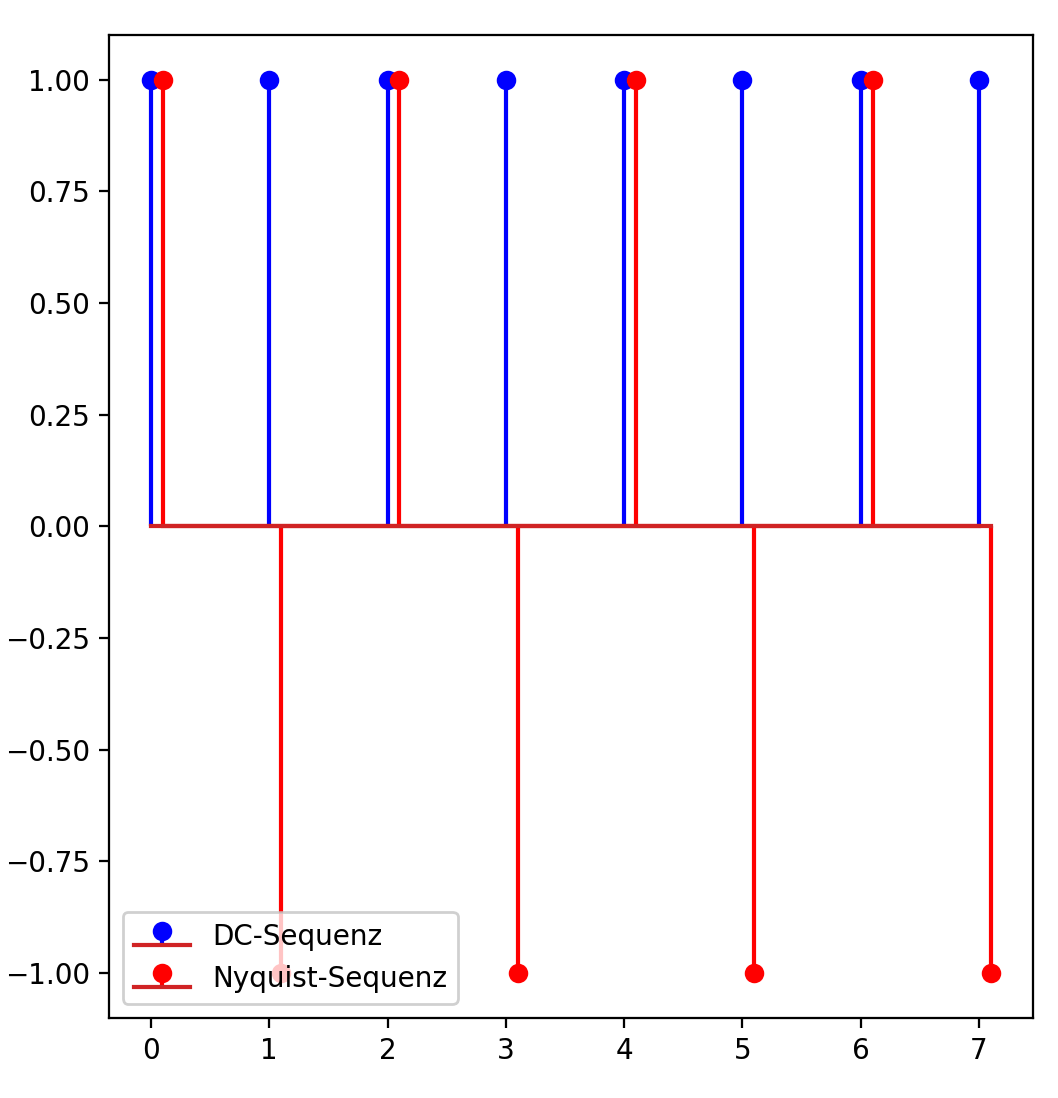
\includegraphics[width=\textwidth]{code/nyquist_seq.png}
    \end{minipage}
    \codecaption{dsv/code/nyquist_seq.py}{Darstellung der DC-Sequenz und der Nyquist-Sequenz f"ur $N=8$}\label{py:nyquist_seq}
\end{listing}

Man in \Cref{py:nyquist_seq} gut, dass die beiden Sequenzen wirklich \q{Gegens"atze} darstellen, da $x_0[\cdot]$ die Anteile mit \q{minimaler} Variation/Frequenz aufsammelt, w"ahrend die Werte von $x_{N/2}[\cdot]$ genau so liegen, dass ein analoges Signal (und dessen Aliase), siehe \Cref{py:aliasing}, genau Frequenz $F_s/2$ (und Amplitude $1$) besitzen muss, um $x_{N/2}[\cdot]$ als Abtastwerte zu erhalten.
%
%
\paragraph{Zyklische Faltung}
%
Kommen wir nun zur wahrscheinlich wichtigsten Eigenschaft der \gls{dft} und dem Grund, warum digitale Signalverarbeitung "uberhaupt erm"oglicht wurde.
Wir haben bereits gesehen, dass \gls{lti}-Systeme durch eine Faltung realisiert werden k"onnen.
Gegeben zwei $N$-periodische Signale $x_{1,2}[\cdot]$ und betrachten wir deren \emph{zyklische} Faltung $\circledast$ definiert durch
\begin{equation}\label{eq:fourier:cyclic_conv}
x_3[m] = \Sum{n=0}{N-1}{x_1[n] \cdot x_2[(m-n) \mod N]} = (x_1 \circledast x_2)[m],
\end{equation}
dann kann man zeigen, dass
\[
X_3[k] = X_1[k] \cdot X_2[k]
\]
gilt.
Das hei"st, dass die zyklische Faltung von zwei periodischen Signalen wieder ein periodisches Signal ergibt, dessen \gls{dft} das Produkt der \glspl{dft} der gefalteten Signale ist.
Wenn wir an \gls{lti}-Systeme denken und uns erinnern, dass viele Filter als \gls{lti}-Systeme aufgefasst werden k"onnen, so ist klar, warum diese Eigenschaft wichtig ist.
Die digitalen Filter k"onnen also im Frequenzbereich sehr einfach angewendet werden, weil dort nur eine einfache punktweise Multiplikation notwendig ist.
Doch dies allein ist nicht ausreichend, denn wir ben"otigen noch einen effizienten weg, um zwischen Zeit- und Freqeunzbereich wechseln zu k"onnen.
Dies wird uns durch die \gls{fft} erm"oglicht werden.
In \Cref{py:dft_1} hatten wir bereits erfahren, dass man die \gls{dft} als Matrix-Vektor-Produkt formulieren kann, wozu etwa \glspl{flop} in der Gr"o"senordnung $N^2$ notwendig sind.
Die \gls{fft} erlaubt es aber eine \gls{dft} mit \glspl{flop} in der Gr"o"senordnung von nur $N \log{N}$ durchzuf"uhren.
%
% \begin{itemize}
%     \item \begin{itemize}
%         \item reelles signal: dc und nyquist reell
%     \end{itemize}
%     \item dft als approximation der dtft
%     \begin{itemize}
%         \item $s(t) = \exp(-t/\tau) \cdot \sin(\omega_0 \cdot t)$, 
%         \item $s(t) = \exp(-(t - \mu)^2/\sigma^2)$ (Uebung)
%     \end{itemize}
% \end{itemize}

%
%
\section{Multiraten Systeme}\label{multirate}
%
\begin{itemize}
    \item system das signale in mehreren raten gleichzeitig benutzt
    \item erste option: digital zu analog, filtenr, analog zu digital
    \item vorteil: sampling rate kann beliebig (je nach signal bandbreite) veraendert werden
    \item nachteil: distortion von da, ad conversion introduce noise, quantization errors
    \item also: conversion direkt in digitaler domaene
    \item problem: how? wir haben das signal nur auf diskreten werten gegeben
    \item wir koennen aber mal die formel fuer perfekte rekonstruktion aufschreiben, die das richtige tut unter der bedingung, dass sampling rate nyquist einhaelt
    \item dann koennen wir diese interpolation einfach auf den neuen samplingpunkten auswerten
    \item resampling ist immerhin schonmal ein lineares system
    \item falls neue samplingrate kleiner, muessen wir auch hier noch nyquist einhalten, oder eben die formel selbst lowpass-filtern
    \item falls alte samplingrate = neue samplingrate haben wir ein LTI-system (uebung)
    \item wenn die samplingrate beliebgi sind, muss man genau hinschauen.
    \item erstmal bild malen
    \item dann gleichungen rumwursten
    \item lineares zeitvariantes system, also impulsantwort ist zeitabhaengig
    \item dann nochmal bild anschauen
    \item fuer rationales verhaeltnis: intuitiv kommt man je nach evrhaltnis wieder auf die gleichen fractional parts, also ist das resampling ein periodisch zeitvariantes lineares system 
    \item downsampling um faktor $D$ (in uebung programmieren, einmal mit weglassen und einmal als faltung)
    \item upsampling um faktor $I$ liefert $I$ verschiedene Impulsantworten des systems
    \item beispiel mit $I = 2$ in der vorlesung (Figure 11.1.4.!), beispiel mit $I = 3$ in uebung. einmal ohne interleaving als periodisch zeitvariantes systen, einmal mit interleaving
\end{itemize}
%
%
\section{STFT}\label{stft}
%
Als erstes wollen wir uns mit der Fourier-Analyse von Signalen besch"aftigen.
Hierbei ist das Ziel das Verhalten eines Signals im Frequenzbereich zu charakterisieren.
Wir wollen jedoch in unserer Analyse davon ausgehen, dass wir ein Signal $x[\cdot]$ vorliegen haben, dessen spektrale Eigenschaften \emph{zeitvariant} sind.
Hiermit ist \emph{nicht} gemeint, dass wir davon ausgehen, dass das Signal zeitvariant ist, denn das ist es nat"urlich.
Es geht darum, dass der Anteil der verschiedenen Frequenzen in einem Signal sich mit der Zeit "andert.
Nat"urlich ist hier eine der am einfachsten zug"anglichen Anwendungen die Analyse von Audiosignalen.

Beginnen wir mit einer intuitiven Betrachtung.
Zun"achst wollen wir einen m"oglichst gro"sen Bereich im Frequenzbereich abdecken -- zumindest den f"ur die jeweilige Anwendung relevanten.
Da sich beispielsweise im Audiobereich oft an der menschlichen H"orcharakteristik orientiert wird, die jenseits von \SI{20}{\kilo\hertz} nichts mehr leistet, sind Frequenzen jenseits dieser Grenze nicht mehr relevant.
Das hei"st, dass sinnvollerweise ein Audiosignal mit einer Sample-Rate von \SI{40}{\kilo\hertz} bereits absolut ausreichend aufgenommen wurde.
F"ur andere Anwendungen lassen sich oft "ahnliche Argumente finden, da die meisten physikalischen Systeme eine Tief- oder Bandpasscharakteristik \q{versteckt} haben, und man somit nur sehr selten mit Signalen mit immensen Bandbreiten konfrontiert ist.
Zusammenfassend muss also die Sample-Rate so angepasst werden, dass sie entsprechend unserer Anforderungen ausreicht.

Dar"uber hinaus ist uns aber auch gut daran getan, die Frequenzen, die in dem Signal vorkommen, sehr gut unterscheiden zu k"onnen.
Wir wollen also m"oglichst \emph{genau} wissen, welche einzelnen Frequenzen im Signal vorhanden sind. 
Das hei"st, dass wir f"ur eine tats"achlich im Signal vorhandene Frequenz $F$ aus unserer Analyse eine Frequenz erhalten wollen, die im Intervall $[F-\Delta_1,F-\Delta_1]$ f"ur m"oglichst kleines $\Delta_1 > 0$ liegt.
In diesem Sinne wollen wir also m"oglichst gro"se \emph{Aufl"osung}.
Wenn wir daran denken, dass $\Delta_1 = F_s/N$ gilt, so scheint es zu helfen, dass wir ein Signal m"oglichst lange \q{beobachten} m"ussen, also $N$ sehr gro"s w"ahlen m"ussen.

Doch es gibt noch einen weiteren Aufl"osungsbegriff, der vom ersten strikt zu unterscheiden ist.
Wir wollen au"serdem eine maximale Trennsch"arfe zwischen zwei unterschiedlichen Frequenzen, die gleichzeitig im Signal vorhanden sind, erreichen.
Wir wollen also in unserer Analyse zwei Frequenzen $F_1$ und $F_2$ mit $\Abs{F_1 - F_2} = \Delta_2$ immernoch unterscheiden k"onnen.
Wiederum ist hier das minimale $\Delta_2 > 0$ von Interesse, f"ur das diese Unterscheidbarkeit noch gilt, da dieses ein weiteres Aufl"osungslimit unseres Systems ist.
"Ahnlich wie bei $\Delta_1$ ist auch hier der Beobachtungszeitraum $N$, welchen wir als Grundlage f"ur unsere Analyse verwenden, von Bedeutung. 
Gr"o"ser Zeitr"aume erlauben eine bessere Aufl"osung \emph{zwischen} Frequenzen.

Au"serdem ist es noch oft interessant, dass man einen hohen Dynamikbereich abdecken kann.
Dies meint, dass man Frequenzanteile mit Frequenzen $F_1$ und $F_2$ und Amplituden $A_1$ und $A_2$ noch als zwei wahrnimmt, solange $\log(A_1/A_2) > \Delta_3$. 
Je gr"o"ser das maximale $\Delta_3$ ist, desto besser, da prominente Frequenzanteile nicht weitere weniger stark ausgepr"agte Anteile maskieren.

Schlussendlich haben wir es auch mit zeitvarianten Frequenzanteilen zu tun.
Das hei"st, dass sich zum Zeitpunkt $T_1$ die Zusammensetzung der Frequenzen von denen zum Zeitpunkt $T_2$ unterscheidet.
F"ur $\Abs{T_1 - T_2} > \Delta_4$ wollen wir also erkennen, dass $x(T_1)$ andere spektrale Charakteristik hat als $x(T_2)$ und die f"ur m"oglichst kleine $\Delta_4$.
Diese zeitliche Evolution des Spektrums ist nat"urlich von immenser Bedeutung, weil man m"oglichst genau wissen m"ochte, \emph{wann} sich Frequenzen im Signal ver"andern.
Ideal w"are es also, wenn wir eine Art \q{instantane} Frequenzanalyse durchf"uhren k"onnten, die trennscharf in einem infinitesimalen Intervall die jeweiligen Frequenzanteile aus dem Signal extrahiert.
Doch Schwingungen sind auf inh"arent \emph{ausgedehnte} Effekte.
Ein kleines $\Delta_4$ steht also in direktem Widerspruch zu den Anforderungen an unsere Analyse f"ur, gute (lies: kleine) $\Delta_1$ und $\Delta_2$, da wir dort gesehen haben, dass wir das Signal \emph{lange} beobachten m"ussen.
F"ur diesen Beobachtungszeitraum nehmen wir aber das Signal als \q{konstant} im Frequenzbereich -- also genau kontraproduktiv f"ur ein kleines $\Delta_4$.
\begin{listing}[ht]
    \noindent
    \begin{minipage}{0.51\textwidth}
        \strut\vspace*{-\baselineskip}\newline
        \inputminted[firstline=10, lastline=44]{python3}{code/stft_1.py}
    \end{minipage}%
    \begin{minipage}{0.48\textwidth}
        \strut\vspace*{-\baselineskip}\newline
        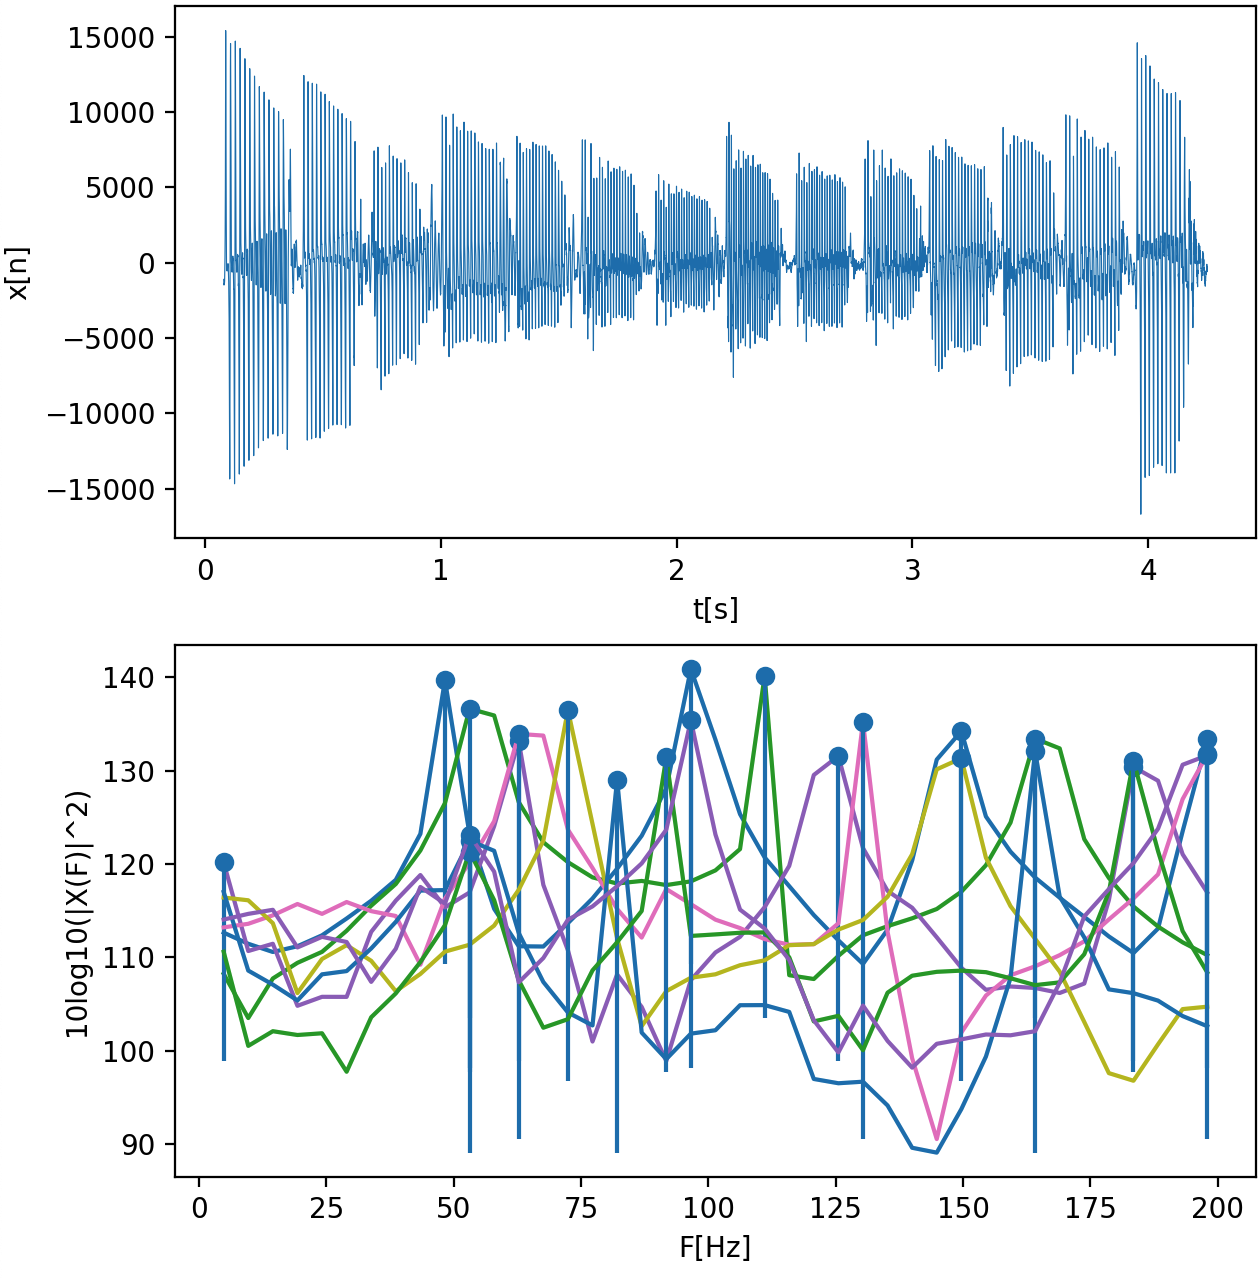
\includegraphics[width=\textwidth]{code/stft_1.png}

\begin{minted}{python}
[ 48.2811  96.5622 149.6715 197.9527]
[ 53.109  111.0466 164.1559]
[  4.8281  62.7654 125.5309 183.4683]
[ 62.7654 130.3590 197.9527]
[ 72.4217 149.6715]
[ 53.109   82.0779 164.1559]
[ 53.109   91.7341 183.4683]
[ 53.109   96.5622 197.95270418]
\end{minted}
    \end{minipage}
    \codecaption{dsv/code/stft_1.py}{Analyse einer \q{Bassline}, die eine G-Dur-Tonleiter spielt.}\label{py:stft_1}
\end{listing}


%
%
\section{Wavelets}\label{wavelets}
%
\begin{itemize}
    \item motivation: analyse in zeit und frequenz gleichzeitig
    \item definition \cite[chpt 4.3, (4.30)]{mallat2008wavelets}
    \item convolution, i.e. linear filter
    \item real heisenberg uncertainty: heisenbergboxes
    \item mexican hat wavelet: second derivative of gaussian
    \item gabor wavelets (uebung)
    \item discrete wavelet transform \cite[ch 4.3.3]{mallat2008wavelets}
\end{itemize}
%
%
\section{B-Splines}\label{bsplines}
%
% !TEX root = ../dsv_script.tex
%
Eine Grundvoraussetzung f"ur eine praktisch n"utzliche digitale Signalverarbeitung ist die M"oglichkeit zwischen dem analogen und digitalen Bereich wechseln zu k"onnen. 
Hierbei sollte man auch genau quantifizieren k"onnen, ob bei diesem Prozess Informationen verloren gehen, oder wie man garantieren kann, dass diese Umwandlung verlustfrei vonstatten geht. 
Meist nutzt man hierf"ur das Sampling \Cref{stm:sampling_theorem}. 
Die hieraus resultierende sogenannte Nyquist-Sampling-Theorie fu"st bekannterma"sen auf der Repr"asentation von bandbegrenzten Signalen durch hinreichend dichte "aquidistante Abtastwerte.

Es gibt jedoch auch einige Nachteile von Nyquist-Sampling, die aus dessen Annahmen und der daraus folgenden Verarbeitung entstehen. 
Einerseits kann ein endliches Signal im Allgemeinen \emph{nicht} bandbegrenzt sein. 
Weiterhin entstehen durch die Bandlimitierung von Signalen Gibbs-Artefakte, siehe \Cref{py:dtft}, die besonders bei der Bilderverarbeitung nicht erw"unscht sind. 
Geht es um die Auswertung $x(t)$ eines Signals $x$ zwischen den aufgenommenen Samples $x[n]$, also um Interpolation, hat man das Problem, dass die $\Sinc$-Funktion nur sehr langsam mit Rate $1/t$ abf"allt.
Diese Eigenschaft f"uhrt dazu, dass man f"ur die Bestimmung eines Wertes $x(t)$ mit einer Genauigkeit von \SI{1}{\percent} etwa $100$ um $t$ benachbarte Samples betrachten muss. 
Das hei"st, vor allem bei 2D-Interpolation, siehe \Cref{sec:dftintp}, skaliert der resultierende Rechenaufwand nicht sehr g"unstig, falls hohe Genauigkeit ben"otigt wird.

Aus diesem Grund m"ochten wir uns eine alternative Sampling-Theorie genauer ansehen -- die B-Splines~\cite{unser1999splines_mag}. 
Wir f"uhren zun"achst die auf Polynomen basierende Signalverarbeitung ein und vergleichen sie anschlie"send zur bereits bekannten Nyquist-Theorie.

\subsection{B-Splines als Polynome}

Allgemein bezeichnet man st"uckweise definierte und stetig differenzierbare Polynome als Splines. 
Man nennt die Stellen an denen zwei unterschiedliche Polynome zusammensto"sen als Knoten. 
Ein Spline der Ordnung $\ell \in \N$ ist ein Polynom vom Grad $\ell$, ist also von der Form
\begin{equation}
    p(t) = 
        a_{\ell} t^{\ell} 
        + a_{\ell - 1} t^{\ell-1} 
        + \dots
        + a_1 t 
        + a_{0}.
\end{equation}
%
Ein Spline ist nun eine Funktion $s(t)$, welche f"ur Knoten $n = 1, 2, \dots$ definiert ist durch
\begin{equation}
    s(t) = \begin{cases}
        p_1(t) \fuer x \in [1,2], \\
        p_2(t) \fuer x \in [2,3], \\
        \vdots
    \end{cases}
\end{equation}
wobei sich die Glattheit durch die Forderung ergibt, dass die Funktion und ihre Ableitungen an den Knoten stetig sei, also
\begin{equation}
    \lim\limits_{t \rightarrow n^-} s^{(m)}(t) =
    \lim\limits_{t \rightarrow n^+} s^{(m)}(t)
\end{equation}
erf"ullt ist, wobei $s^{(m)}$ f"ur $m \geqslant 0$ die $m$-te Ableitung des Splines $s$ repr"asentiert. 
In einer Arbeit~\cite{schoenberg1988bsplines}, die sogar dem ber"uhmten Paper von Shannon vorausgeht, beschreibt Schoenberg, dass sich diese Splines der Ordnung $\ell$ via
\begin{equation}\label{eq:bsplines:summation}
    s(t) = \Sum{k \in \Z}{}{
        c[k] \beta^{\ell}(t - k)
    }
\end{equation}
darstellen lassen. Hierbei ist die Funktion $\beta^\ell: \R \rightarrow \R$ definiert als eine iterierte Faltung einer Rechteck-Funktion via
\begin{equation}
    \beta^\ell = \underbrace{
        \beta^0 \ast \dots \ast \beta^0
    }_{(\ell+1) \Text{mal}}, 
    \Text{wobei}
    \beta^0(t) = \begin{cases}
        1,\quad \Abs{t} < \frac{1}{2} \\
        \frac{1}{2}, \quad \Abs{t} = \frac{1}{2} \\
        0, \Text{sonst.}
    \end{cases}
\end{equation}
In \Cref{fig:bsplines:all_splines} sind die Funktionen $\beta^\ell$ f"ur $\ell = 0, \dots, 3$ dargestellt. 
Man erkennt sehr gut, dass der Grad der Glattheit von der Ordnung des Splines abh"angt und dass die Funktionswerte $\beta^\ell(t)$ f"ur $\Abs{t}>\ell+1/2$ verschwinden. 
Man spricht von Funktionen mit \emph{kompaktem Tr"ager}. 
Das hei"st die Summation in \eqref{eq:bsplines:summation} ist f"ur fixes $t \in \R$ \emph{endlich} und ist auf $\ell+1$ Summanden beschr"ankt!
%
\begin{figure}
    \centering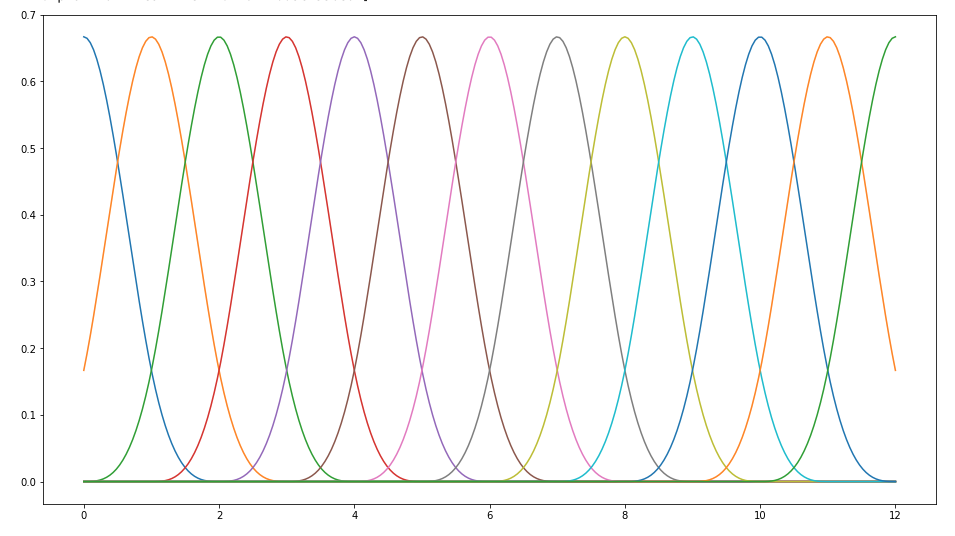
\includegraphics[width=0.9\textwidth]{img/bsplines/all_splines.png}
    \caption{Kubische B-Splines f"ur Abtastung an den Werten $n = 0, \dots, 12$.}\label{fig:bsplines:all_splines}
\end{figure}
%
Wir wollen nun eine explizite Formel f"ur $\beta^\ell$ entwickeln. Hierzu betrachten wir die Fourier-Transformation 
\begin{equation}
    B^\ell(\omega) 
        = \left(\frac{\sin(\omega / 2)}{(\omega / 2)}\right)^{\ell + 1}
        = \frac{(\exp(\jmath \omega/2) - \exp(-\jmath \omega/2))^{\ell+1}}{
            (\jmath \omega)^{\ell + 1}
        }
\end{equation}
mit einigen Rechentricks (siehe \cite[Box 1.]{unser1999splines_mag}) kann man dies so lange umformen, bis man
\begin{equation}
    \beta^\ell(t) = \frac{1}{\ell !}\Sum{p = 0}{\ell+1}{
            \binom{\ell+1}{p}(-1)^p
            \left(t - p + \frac{\ell+1}{2}\right)_+^\ell
        }
    \Text{mit}
    (x)_+ = \begin{cases}
      x, \fuer x \geqslant 0, \\
      0, \Text{sonst},  
    \end{cases}
\end{equation}
erh"alt. 
Damit ist $\beta^\ell$ wirklich ein Polynom $\ell$-ten Grades. 
Die Stetig- und Differenzierbarkeit muss man sich aber noch separat "uberlegen. 

Weiterhin kann man zeigen, dass folgende Formeln f"ur Differentiation und Integration von B-Splines gelten:
\begin{equation}\label{eq:bsplines:deriv_int}
    \left(\beta^\ell\right)^\prime(t) =
        \beta^{\ell-1}(t + 1/2) - \beta^{\ell-1}(t - 1/2), 
    \Int{-\infty}{t}{\beta^\ell(s)}{s} = 
        \Sum{p = 0}{+\infty}{\beta^{\ell+1}(t - 1/2 - p)}.
\end{equation}
Das hei"st, dass man auch einen kompletten Spline $s$ differenzieren und integrieren kann, indem man nutzt, dass sowohl Differentiation, als auch Integration lineare Operationen sind. 
Es gilt also mit \eqref{eq:bsplines:summation} und \eqref{eq:bsplines:deriv_int} beispielsweise f"ur die Differentiation, dass
\begin{equation}
    s^\prime(t) = \Sum{k \in \Z}{}{
        c[k] \left(\beta^{\ell}\right)^\prime(t - k)
    }
    = \Sum{k \in \Z}{}{
        c[k]\left(
            \beta^{\ell-1}(t + 1/2 - k) - \beta^{\ell-1}(t - 1/2 - k)
        \right)
    }.
\end{equation}
%
Diese Eigenschaft macht man sich auch f"ur kompliziertere Operationen, wie Rotationen und Verzerrungen auf einem Spline $s$ zunutze.
%
%
\subsection{Kubische B-Spline Interpolation}
%
%
Wir m"ochten uns eine spezielle Version der B-Splines genauer Ansehen, da diese in der Anwendung den Spagat zwischen Komplexit"at und Approximationsg"ute sehr gut hinbekommen. 
Wir setzen hierzu $\ell=3$ und erhalten somit ein Polynom dritten Grades der Form
\begin{equation}\label{eq:bsplines:explicit_eval}
    \beta^3(t) = \begin{cases}
        \frac 23 - \Abs{t}^2 + \frac{\Abs{t}^3}{2} \fuer \Abs{t} < 1\\
        \frac{(2 - \Abs{t})^3}{6}, \fuer \Abs{t} \in [1, 2) \\
        0, \fuer \Abs{t} > 2,
    \end{cases}
\end{equation}
welche in \Cref{py:bsplines:eval} auch einmal implementiert wurde. 

\begin{listing}
\inputminted[firstline=4]{python}{code/bsplines_eval.py}
\codecaption{dsv/code/bsplines_eval.py}{Implementierung von \eqref{eq:bsplines:explicit_eval}}\label{py:bsplines:eval}            
\end{listing}

In Analogie zum bekannten Nyquist-Sampling wollen wir untersuchen, wie wir aus endlich vielen gegebenen Abtastwerten $x[n]$ mit $n \leqslant N$ eine Darstellung wie in \eqref{eq:bsplines:summation} herleiten k"onnen, welche die abgetasteten Werte exakt interpoliert. Aufgabe ist es also aus $x[n]$ die Folge $c[k]$ zu bestimmen.

Hierzu ben"otigen wir die sogenannte Interpolationsbedingung, siehe \eqref{eq:dftintp:interpol_cond}, welche f"ur eine zu interpolierende Funktion $x$ und ihre Abtastwerte $x[n] = x(n)$ fordert, dass
\begin{equation}\label{eq:bsplines:interpol_cond}
    x(n) = x[n] = s(n) = \Sum{k \in \Z}{}{
        c[k] \beta^{3}(n - k)
    }
\end{equation}
gilt. 
Wir fordern also \emph{exakte} Interpolation. 
Nun k"onnte man f"ur die Bestimmung der Folge $c[k]$ ein lineares Gleichungssystem aufstellen, welches die Form
%
\begin{equation}\label{eq:bsplines:lse}
    \bm B \cdot \bm c = \bm x
\end{equation}
%
hat, wobei die Systematrix $\bm B$ durch die Auswertung der B-Splines an den Stellen $n$ bestimmt ist und der Vektor $\bm x$ den Werten $x[n]$ entspricht. 
Dem endlichen Tr"ager der Funktionen $\beta^\ell$ ist es zu verdanken, dass die Matrix $B$ mit nur wenigen von $0$ verschiedenen Werten besetzt ist (genauer: band-diagonal) und demzufolge effizient invertierbar ist.
Es ist also nicht \q{schwer} $\bm c = \bm B^{-1} \bm y$ zu berechnen. 
Doch die Anwendung von $B^{-1}$ ist numerisch instabil, weshalb wir einen alternativen Weg einschlagen, der auf inverser Filterung beruht.

Sehen wir uns \eqref{eq:bsplines:interpol_cond} genauer an. 
Wir finden, dass sich diese Gleichung nach Definition von $\beta[k] = \beta^3(k)$ als Faltung via
\begin{equation}\label{eq:bsplines:conv}
    x[n] = (c \ast b)[n]
\end{equation}
schreiben l"asst. 
Nach Transformation in den $z$-Bereich erhalten wir
\begin{equation}\label{eq:bsplines:ztrafo}
    X(z) = C(z) \cdot B(z) \Rightarrow C(z) = \frac{X(z)}{B(z)},
\end{equation}
was uns motiviert eine Darstellung von $1/B(z)$ im Zeitbereich herzuleiten. 
F"ur die kubischen B-Splines folgt, dass
\begin{equation}\label{eq:bsplines:filter}
    B(z) = \frac{z + 4 + z^{-1}}{6} 
    \Rightarrow \frac{1}{B(z)} 
        = 6 \left(\frac{1}{1 - z_1 z^{-1}}\right) \left(\frac{-z_1}{1 - z_1 z}\right)
\end{equation}
gilt. 
Wobei man zeigen kann, dass $z_1 = \sqrt{3} - 2 < 1$ gilt. 
Wir betrachten nun $1/B(z)$ als einen Filter, der auf die Abtastwerte $x[n]$ angewandt werden soll. 
Aus \eqref{eq:bsplines:filter} erkennen wir, dass $1/B(z)$ ein Filter ohne Nullstellen ist und als Hintereinanderausf"uhrung von zwei rekursiven Filtern betrachtet werden kann. 
Wir erhalten mit $c^{-}[k] = c[k]/6$, dass sich $1/B(z)$ durch
\begin{align}
    c^+[k] &= 
        x[n] + z_1 c^+[k-1] \fuer k = 1, \dots N-1 \\
    -c[k]/6 = c^-[k] &= 
        z_1\left( c^{-}[k+1] - c^+[k]\right) \fuer k = N-2, \dots, 0
\end{align}
ausdr"ucken l"asst. 
Diese Methode der kausalen und anti-kausalen Filterung ist deutlich effizienter und stabiler, als \eqref{eq:bsplines:lse}, da beispielsweise keine Divisionen notwendig sind. 
Nun ist es noch notwendig Anfangswerte f"ur $c^+[k]$ und $c^-[k]$ zu finden. 
Dies ist aufgrund der Endlichkeit von $x$ nicht ohne Weiteres m"oglich. 
Man sieht, dass die Impulsantwort von $c^+$ eine abklingende Exponentialfunktion ist, also gilt
\begin{equation}
    c^+[0] = \Sum{k=0}{\infty}{x[-k] z_1^k} \approx \Sum{k=0}{K}{x[-k] z_1^k},
\end{equation}
wobei man $K \in \N$ so w"ahlen kann, dass $z_1^K \leqslant \varepsilon$ erf"ullt ist, siehe \Cref{py:exp_mean}.
Nach Ausf"uhrung von $c^+$ kann man $c^-[N-1]$ durch
\begin{equation}
    c^-[N-1] = \frac{z_1}{1 - z_1^2}\left(c^+[N-1] + z_1 c^+[N-2]\right)
\end{equation}
effizient und exakt initialisieren. 
Beides wurde in \Cref{py:bsplines:coeffs} beispielhaft implementiert und eine m"ogliche Ausgabe nach Auswertung von \eqref{eq:bsplines:summation} ist in \Cref{fig:bsplines:interpol} dargestellt.
%
\begin{listing}[t]
\inputminted[firstline=4]{python3}{code/bsplines_coeffs.py}
\codecaption{dsv/code/bsplines_coeffs.py}{Berechnung der B-Spline Koeffizienten}\label{py:bsplines:coeffs}
\end{listing}
%
\begin{figure}[t]
    \centering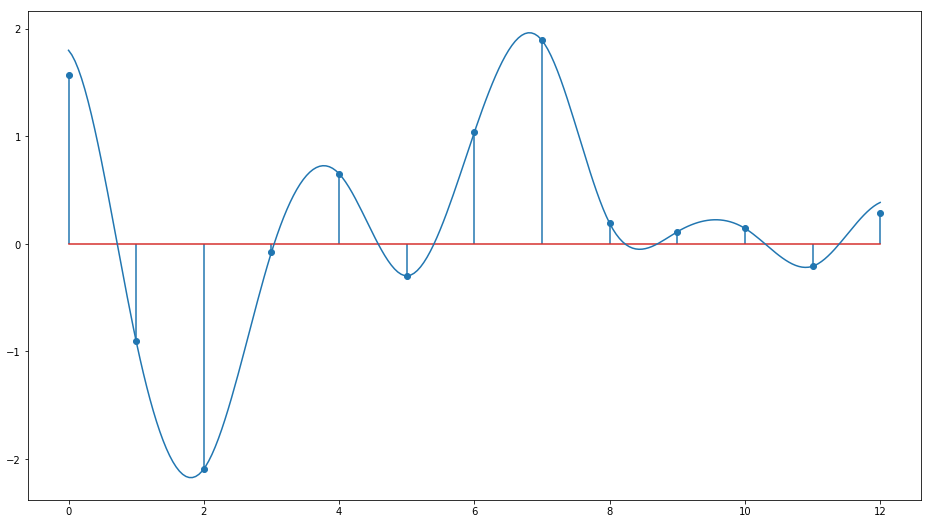
\includegraphics[width=0.9\textwidth]{img/bsplines/interpol.png}
    \caption{Kubische B-Spline-Interpolation f"ur Abtastung an den Werten $n = 0, \dots, 12$.}\label{fig:bsplines:interpol}
\end{figure}
%
%
%
\subsection{Verbindung zur Nyquist-Sampling-Theorie}
%
%
Wir wollen als Abschluss eine Verbindung zum Sampling und der Interpolation~\cite[Kapitel~6.1]{proakis2013} von bandbegrenzten Funktionen mit endlicher Energie ziehen. 
Nehmen wir als Wiederholung zun"achst an, dass das bandbegrenzte Signal $x_a$ mit endlicher Energie und Fourier-Transformation $X_a$ mindestens kritisch mit Rate $F_s$ zu den Werten $x[n]$ abgetastet wurde. 
Wir bezeichnen mit $X$ die \gls{dtft} von $x[n]$. Dann gilt als Zusammenhang zwischen den beiden Spektra, wie in \Cref{sec:sampling:sampling_theorem}, dass
\begin{equation}
    X(f) = F_s \Sum{k=-\infty}{+\infty}{
        X_a((f - k) F_s)
    },
\end{equation}
was die Periodifizierung des Frequenzbereiches durch Abtastung ausdr"uckt. 
Nach Annahme der kritischen Abtastung findet hier kein Aliasing statt, sodass f\u"r $f \in [-F_s/2,+F_s/2]$ gilt, dass $F_s \cdot X_a(f) = X(f)$. 
Au"serdem k"onnen wir das Spektrum der abgetasteten Werte $X$ durch
\begin{equation}
    X(f) = \Sum{n=-\infty}{+\infty}{x[n] \exp(- \jmath 2 \pi f n / F_s)}
\end{equation}
ausdr"ucken. 
Nun k"onnen wir das analoge Signal $x_a$ in Abh"angigkeit von den Abtastwerten darstellen. 
Es gilt mit $T = 1/F_s$ und nach \Cref{stm:sampling_theorem}, dass
\begin{align*}
    x_a(t) = \Sum{n=-\infty}{+\infty}{
        x[n] \frac{\sin(\pi(t-nT)/T)}{\pi(t-nT)/T}
    }.
\end{align*}
Das hei"st, dass die Funktion $g: \R \rightarrow \R$ mit
\begin{equation}\label{eq:bsplines:sinckernel}
    g(t) = \frac{\sin(\pi t / T)}{(\pi t/T)}
\end{equation}
als \emph{Interpolations-Kernel} von bandbegrenzten und abgetasteten Funktionen betrachtet werden kann. 
Siehe \Cref{sec:eadf} f"ur eine Anwendung dieser Art der Interpolation.

Nun k"onnen wir eine analoge Rechnung f"ur die B-Splines durchf"uhren, indem wir einen Filter $b^{-1}[k]$ als inverse $Z$-Transformation von $1/B(z)$ aus \eqref{eq:bsplines:ztrafo} definieren. 
Dann gilt
\begin{equation}
    c[k] = (b^{-1} \ast x)[k],
\end{equation}
was wir in \eqref{eq:bsplines:interpol_cond} einsetzen und dann
\begin{equation}
    s(t) = \Sum{n \in \Z}{}{
        (b^{-1} \ast x)[n] \beta^{\ell}(t - n)
    } = \Sum{n \in \Z}{}{
        x[n] \Sum{p \in \Z}{}{
            b^{-1,\ell}[p] \beta^{\ell}(t - n - p)
        }
    } = \Sum{n \in \Z}{}{
        x[n] h^\ell(t - n)
    }
\end{equation}
erhalten, wobei wir analog zu \eqref{eq:bsplines:sinckernel} den Interpolationskernel $h: \R \rightarrow \R$ durch
\begin{equation}\label{bsplines_kernel}
    h^\ell(t) = \Sum{p \in \Z}{}{
        b^{-1,\ell}[p] \beta^{\ell}(t - p)
    }
\end{equation}
definiert haben. 
Man kann zeigen, dass $\lim_{l \rightarrow \infty} h^\ell = g$. 
Das hei"st, dass die $\Sinc$-Interpolation als Grenzwert der B-Spline Interpolation aufgefasst werden kann -- oder andersherum -- die B-Spline-Interpolation als Approximation der $\Sinc$-Interpolation. 
Das hei"st, dass auch im Frequenzbereich Konvergenz in der Form
\begin{equation}
    H^\ell(\omega) = \left(\frac{\sin(\omega/2)}{\omega/2}\right)^{\ell+1} \frac{1}{B^{\ell}(\exp(\jmath \omega))} \rightarrow_{\ell \rightarrow \infty} \Rect(\omega)
\end{equation} 
gegeben sein muss.

Zusammenfassend kann man sagen, dass B-Splines einen alternativen Zugang zu digitaler Signalverarbeitung bieten, welcher eng mit dem des Nyquist-Samplings verkn"upft ist und als Approximation von diesem gesehen werden kann. 
B-Splines sind wegen ihrer effizienten und stabilen Implementierung sowohl bei der Analyse \eqref{eq:bsplines:filter}, als auch der Synthese \eqref{eq:bsplines:summation} vor allem f"ur hochdimensionale Interpolationen sehr interessant\linkfootnote{https://developer.nvidia.com/gpugems/gpugems2/part-iii-high-quality-rendering/chapter-20-fast-third-order-texture-filtering}.

%
%
\section{Zuf\"allige Signale}\label{random}
%
Bisher waren wir ausschließlich mit deterministischen Signalen befasst. 
Also solchen, welche sich bequem durch eine Funktionsvorschrift $t \mapsto x(t)$ beschreiben lassen.
Doch eigentlich ist dies ein absolut idealisierter Spezialfall, da für gew\"ohnlich alle Signale, die wir verarbeiten, zu mindestens einem Zeitpunkt von einem Messgerät beobachtet wurden.
Somit sind diese notwendigerweise mit Messrauschen behaftet, dessen unangenehme Eigenschaft es ist, zuällig zu sein.
Aus diesem Grund ist es uns nicht m\"oglich, ein gemessenes und digitalisiertes Signal $x[\cdot]$ mittels eines alebraischen Ausdrucks zu beschreiben.
Notwendigerweise wird $x[\cdot]$ zu einer sog. Zufallsgr\"oße, welche wir \q{nur} noch durch deren statistische Eigenschaften beschreiben k\"onnen.
Nicht nur das, auch jede folgende Verarbeitung von $x[\cdot]$, bespielsweise durch ein \gls{lti}-System, wird zu einer Zufallsgr\"oße, deren Eigenschaften u.A. von denen des Messrauschens abhängen.

Weiterhin kann es für gewisse Anwendungen auch absolut ausreichend sein, eigentlich deterministische Signale als zufällig zu modellieren.
Wenn es beispielsweise darum geht, zu bestimmen, ob ein Kommunikationssystem in der Lage ist, Informationen fehlerfrei zu übertragen, dann kann es ausreichend sein, \q{nur} eine Ausfallrate zu bestimmen, oder diese Rate zu begrenzen, anstatt dies für jedes m\"ogliche übertragene Signal zu bestimmen/gewährleisten.

Um diese \q{neue} Sichtweise auf Signale gut verinnerlichen zu k\"onnen, ben\"otigen wir jedoch einige Werkzeuge aus der Wahrscheinlichkeitstheorie, die wir uns nun ansehen werden, wobei wir versuchen, uns nicht mit vielen mathematischen Details aufzuhalten, sondern wollen stattdessen unsere Intuition schärfen.

\subsection{Grundlagen Wahrscheinlichkeitstheorie}\label{sec:random:prbly}

Nehmen wir zunächst einmal an, dass wir einen zufälligen Vorgang betrachten, dessen Ausgang sich in Form einer einzelnen reellen Zahl manifestiert.
Diesen zufälligen Vorgang assoziieren wir mit der Zufallsgr\"oße $X : \Omega \rightarrow \R$, also $\omega \rightarrow X(\omega)$, wobei wir uns vorstellen, dass $\Omega$, beziehungsweise $\omega$, dafür sorgen, dass Zufall ins Spiel kommt. \textit{$\ast$MITHÄNDENWEDEL$\ast$} Wir sind nun daran interessiert, wie die \emph{Verteilung} der Werte $X(\omega)$ charakterisiert werden kann.

Hierzu definieren wir beigeordnet zu $X$ eine Funktion $F_X: \R \rightarrow [0,1]$, welche uns für $x \in \R$ mitteilt, was die Wahrscheinlichkeit für das Ereignis $X \leqslant x$ ist.
Man kann auch sagen/schreiben:
\[
F_X(x) = P(X \leqslant x).
\]
Die Funktion $F$ ist monoton wachsend, da natürlich $P(X \leqslant x_1) \leqslant P(X \leqslant x_2)$, falls $x_1 < x_2$, also auch $F_X(x_1) \leqslant F_X(x_2)$.
Jetzt kann man mit der \emph{Verteilungsfunktion} $F_X$ schon eine Menge anfangen.
Beispielsweise k\"onnen wir damit auch bestimmen, mit welcher Wahrscheinlichkeit das Ereignis $x_1 < X \leqslant x_2$ eintritt, indem wir einfach 
\[
P(x_1 < X \leqslant x_2) = F_X(x_2) - F_X(x_1)
\]
berechnen.

Wir k\"onnen sogar noch einen Schritt weiter gehen, und die Gr\"oße
\[
f^h_X(x) = \frac{F_X(x + h) - F_X(x)}{h}
\]
betrachten.
Man kann es sich so vorstellen, dass wir das Intervall $[x,x+h]$ hernehmen, berechnen, wie \q{viel} von $X$ in $[x,x+h]$ landen kann, und normieren das mit der Intervallbreite $h$.
Im Grunde berechnen wir, wie \q{dicht} die Zufallsgr\"oße zwischen $x$ und $x+h$ ist.
Aus diesem Grund nennt man
\[
f_X(x) = \lim\limits_{h \rightarrow 0} f^h_X(x) = \lim\limits_{h \rightarrow 0} \frac{F_X(x + h) - F_X(x)}{h}
\]
die \emph{Dichte} von $X$.
Natürlich sehen wir, dass der berechnete Grenzwert der sogenannte Differenzenquotient der Verteilungsfunktion $F_x$ ist. Es gilt also $f_X = F^\prime_X$.
Deshalb kann man nun die Verteilungsfunktion auch aus der Dichte gewinnen, indem wir
\[
F_X(x) = \Int{-\infty}{x}{f_X(s)}{s}
\]
auswerten.
Die obigen Betrachtungen gelten freilich nur, wenn die formulierten Grenzwerte auch immer existieren, doch erstens existieren diese meistens und für ein intuitives Verständnis sollte es zunächst genügen.

Weiterhin gilt für reelle Zufallsgrößen $X$, dass diese sich \q{irgendwo} zwischen $-\infty$ und $+\infty$ mit Wahrscheinlichkeit $1$ realisieren muss.
Also gilt
\[
\lim_{x \rightarrow \infty} F_X(x) = 1,
\]
was für die Dichte ergibt, dass
\[
\Int{-\infty}{+\infty}{f_X(s)}{s} = 1.
\]
%
%
\subsubsection{Beispiele}
%
\paragraph{Uniforme Verteilung/Gleichverteilung}
Gegeben zwei reelle Zahlen $a < b$ nennt man eine Zufallsgröße $X$ verteilt nach $\Unif(a,b)$, wenn die Dichte $f_X$ gegeben ist durch
\[
f_X(x) = \begin{cases}
    0, \Text{falls} x<a, \\
    1/(b-a), \Text{falls} a \leqslant x < b \\
    0, \Text{falls} b \leqslant x.
\end{cases} = 
    \frac 1{b-a} \Rect\left(\frac{x-(b+a)/2}{b-a}\right)
\]
Der Name dieser Verteilung ergibt sich daraus, dass intuitiv alle Intervalle, die im Intervall $[a,b]$ liegen mit einr Wahrscheinlichkeit proportional zu ihrer \q{Länge} von $X$ \q{getroffen} werden.
Man schreibt auch oft $X \sim \Unif(a,b)$.
%
\paragraph{Normalverteilung}
Gegeben zwei Parameter $\mu \in \R$ und $\sigma^2 \in \R^+$, so nennt man eine Zufallsgröße $X$ normalverteilt mit Erwartungswert $\mu$ und Varianz $\sigma^2$, falls deren Dichte $f_X$
\[
f_X(x) = \frac{1}{\sqrt{2 \pi \sigma^2}} \exp\left(-\frac{(x - \mu)^2}{2 \sigma^2}\right)
\]
erfüllt.
Die Normalverteilungist eine sehr wichtige Verteilung, weil aus Gründen die meisten Messwerte einer Normalverteilung mit Erwartungswert $\mu$ und einer gewissen Varianz $\sigma^2$ folgen.
Je größer $\sigma^2$, desto stärker ist die Streuung der gemessenen Werte um den Erwartungswert $\mu$.
Man schreibt auch $X \sim \mathcal{N}(\mu, \sigma^2)$.
Es sind zwei Beispiele in \Cref{py:random:normal1} zusammen mit der Berechnung der Dichte via \texttt{scipy} dargestellt.
Auch hier ist es wieder ratsam, keine eigenen Implementierungen solcher Standardfunktionen zu nutzen und stattdessen auf Funktionen aus getesteten Paketen zurück zu greifen.
\begin{listing}[ht]
    \noindent
    \begin{minipage}{0.51\textwidth}
        \strut\vspace*{-\baselineskip}\newline
        \inputminted[firstline=3, lastline=10]{python3}{code/random/normal1.py}
    \end{minipage}%
    \begin{minipage}{0.48\textwidth}
        \strut\vspace*{-\baselineskip}\newline
        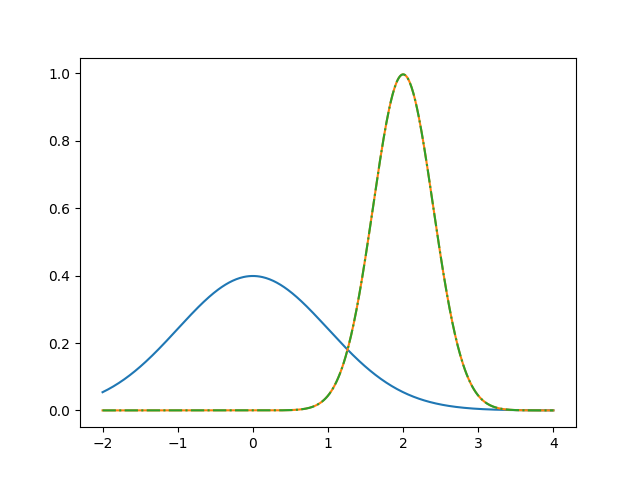
\includegraphics[width=\textwidth]{code/random/normal1.png}
    \end{minipage}
    \codecaption{dsv/code/random/normal1.py}{Visualisierung der Dichte der Normalverteilung für verschiedene Parameter}\label{py:random:normal1}
\end{listing}
%
%
\paragraph{Exponentialverteilung}
Gegeben eine Intensität $\lambda > 0$, so folgt eine Zufallsgröße $X$ einer Exponentialverteilung $\Exp(\lambda)$, falls die Dichte $f_X$ die Form 
\[
f_X(x) = \begin{cases}
    \lambda \exp(-\lambda x), \Text{für} x \geqslant
    0, \\
    0 \Text{sonst}
\end{cases}
\]
besitzt.
Auch eine wichige Verteilung, die beispielsweise die Lebensdauer von irgendwelchen Bauteilen modelliert, oder auch die Wartezeit zwischen zwei Anrufen bei einer Servicehotline. 
Je kleiner $\lambda$, desto höher die Intensität, also desto kürzer die Wartezeit.
%
%
\subsubsection{Erwartungswert, Varianz, Kovarianz}

Will man eine Zufallsgröße auf einige wenige Kennzahlen herunterbrechen, die in der Praxis auch relevant sein könnten, so bieten sich sogenannte Momente deren Verteilung an.
%
%
\paragraph{Erwartungswert}
Interessiert man sich für den Wert, der sich \q{im Mittel} bei einer Verteilung $X$ ergibt, so berechnet man den Erwartungswert $\E(X)$ definiert durch
\begin{equation}\label{eq:random:mean}
    \E(X) = \Int{-\infty}{+\infty}{x f_X(x)}{x}.
\end{equation}
Wenn $f_X$ einer physikalischen Dichteverteilung im Raum entspräche, so würde $\E(X)$ genau den Masseschwerpunkt dieser Verteilung darstellen.
Ist beispielsweise $X \sim \Unif(a,b)$, so gilt $\E(X) = (a+b)/2$ und falls $X \sim \mathcal{N}(\mu, \sigma^2)$, so gilt $\E(X) = \mu$.
%
%
\paragraph{Varianz}
%
Basierend auf dem Erwartungswert, können wir auch die erwartete Streuung einer Zufallsgröße um $\E(X)$ herum betrachten, also
%
\begin{equation}\label{eq:random:var}
\Var(X) 
    = \E((X - \E(X))^2) 
    = \Int{-\infty}{+\infty}{(x-\E(X))^2 f_X(x)}{x}
    = \E(X^2) - \E(X)^2.
\end{equation}
%
Die Interpretation ist, dass $\Var(X)$ die mittlere quadratische Abweichung einer Zufallsgröße von ihrem Erwartungswert beschreibt.
Es ist anzumerken, dass es Verteilungen gibt, für welche $\E$ und $\Var$ nicht existieren müssen, weil die jeweiligen Integrale in \eqref{eq:random:mean} und \eqref{eq:random:var} nicht endlich sind.

Beispielsweise gilt im Falle von $X \sim \Unif(a,b)$, dass $\Var(X) = (b-a)^2/12$ und im Falle von $X \sim \mathcal{N}(\mu, \sigma^2)$, dass $\Var(X) = \sigma^2$.

\subsection{Zufällige Signale}

% - Stochastische Prozesse: definition, zwei sichtweisen (per pfad, folge von verteilungen)
% - stationaere prozesse/signale
% - Wiener-Chintschin-Theorem

\subsection{Parameterschätzung}\label{sec:random:paramest}

\subsection{Quantisierung}\label{sec:random:quanti}

% - \cite{widrow2008quantization}
% - area sampling (geoemetrisch)
% - charakteristische funktion: value at 0, conj sym, 
% - areasampling: analytisch in value domain, in frequ domain
% - reconstruction der PDF aus der quantisierten PDF
% - PQN Model
%
%
%
%
%
\clearpage
\microtypesetup{protrusion=false}
\addcontentsline{toc}{section}{Abk"urzungsverzeichnis}
\printglossary[type=\acronymtype]
\microtypesetup{protrusion=true}
%
%
%
\clearpage
\microtypesetup{protrusion=false}
\addcontentsline{toc}{section}{Literaturverzeichnis}
\printbibliography
\microtypesetup{protrusion=true}
\end{document}